\documentclass[twoside]{book}

% Packages required by doxygen
\usepackage{fixltx2e}
\usepackage{calc}
\usepackage{doxygen}
\usepackage[export]{adjustbox} % also loads graphicx
\usepackage{graphicx}
\usepackage[utf8]{inputenc}
\usepackage{makeidx}
\usepackage{multicol}
\usepackage{multirow}
\PassOptionsToPackage{warn}{textcomp}
\usepackage{textcomp}
\usepackage[nointegrals]{wasysym}
\usepackage[table]{xcolor}

% Font selection
\usepackage[T1]{fontenc}
\usepackage[scaled=.90]{helvet}
\usepackage{courier}
\usepackage{amssymb}
\usepackage{sectsty}
\renewcommand{\familydefault}{\sfdefault}
\allsectionsfont{%
  \fontseries{bc}\selectfont%
  \color{darkgray}%
}
\renewcommand{\DoxyLabelFont}{%
  \fontseries{bc}\selectfont%
  \color{darkgray}%
}
\newcommand{\+}{\discretionary{\mbox{\scriptsize$\hookleftarrow$}}{}{}}

% Page & text layout
\usepackage{geometry}
\geometry{%
  a4paper,%
  top=2.5cm,%
  bottom=2.5cm,%
  left=2.5cm,%
  right=2.5cm%
}
\tolerance=750
\hfuzz=15pt
\hbadness=750
\setlength{\emergencystretch}{15pt}
\setlength{\parindent}{0cm}
\setlength{\parskip}{3ex plus 2ex minus 2ex}
\makeatletter
\renewcommand{\paragraph}{%
  \@startsection{paragraph}{4}{0ex}{-1.0ex}{1.0ex}{%
    \normalfont\normalsize\bfseries\SS@parafont%
  }%
}
\renewcommand{\subparagraph}{%
  \@startsection{subparagraph}{5}{0ex}{-1.0ex}{1.0ex}{%
    \normalfont\normalsize\bfseries\SS@subparafont%
  }%
}
\makeatother

% Headers & footers
\usepackage{fancyhdr}
\pagestyle{fancyplain}
\fancyhead[LE]{\fancyplain{}{\bfseries\thepage}}
\fancyhead[CE]{\fancyplain{}{}}
\fancyhead[RE]{\fancyplain{}{\bfseries\leftmark}}
\fancyhead[LO]{\fancyplain{}{\bfseries\rightmark}}
\fancyhead[CO]{\fancyplain{}{}}
\fancyhead[RO]{\fancyplain{}{\bfseries\thepage}}
\fancyfoot[LE]{\fancyplain{}{}}
\fancyfoot[CE]{\fancyplain{}{}}
\fancyfoot[RE]{\fancyplain{}{\bfseries\scriptsize Generated by Doxygen }}
\fancyfoot[LO]{\fancyplain{}{\bfseries\scriptsize Generated by Doxygen }}
\fancyfoot[CO]{\fancyplain{}{}}
\fancyfoot[RO]{\fancyplain{}{}}
\renewcommand{\footrulewidth}{0.4pt}
\renewcommand{\chaptermark}[1]{%
  \markboth{#1}{}%
}
\renewcommand{\sectionmark}[1]{%
  \markright{\thesection\ #1}%
}

% Indices & bibliography
\usepackage{natbib}
\usepackage[titles]{tocloft}
\setcounter{tocdepth}{3}
\setcounter{secnumdepth}{5}
\makeindex

% Hyperlinks (required, but should be loaded last)
\usepackage{ifpdf}
\ifpdf
  \usepackage[pdftex,pagebackref=true]{hyperref}
\else
  \usepackage[ps2pdf,pagebackref=true]{hyperref}
\fi
\hypersetup{%
  colorlinks=true,%
  linkcolor=blue,%
  citecolor=blue,%
  unicode%
}

% Custom commands
\newcommand{\clearemptydoublepage}{%
  \newpage{\pagestyle{empty}\cleardoublepage}%
}

\usepackage{caption}
\captionsetup{labelsep=space,justification=centering,font={bf},singlelinecheck=off,skip=4pt,position=top}

%===== C O N T E N T S =====

\begin{document}

% Titlepage & ToC
\hypersetup{pageanchor=false,
             bookmarksnumbered=true,
             pdfencoding=unicode
            }
\pagenumbering{alph}
\begin{titlepage}
\vspace*{7cm}
\begin{center}%
{\Large Object Detection \\[1ex]\large 4.\+0 }\\
\vspace*{1cm}
{\large Generated by Doxygen 1.8.13}\\
\end{center}
\end{titlepage}
\clearemptydoublepage
\pagenumbering{roman}
\tableofcontents
\clearemptydoublepage
\pagenumbering{arabic}
\hypersetup{pageanchor=true}

%--- Begin generated contents ---
\chapter{Todo List}
\label{todo}
\Hypertarget{todo}

\begin{DoxyRefList}
\item[\label{todo__todo000001}%
\Hypertarget{todo__todo000001}%
Class \hyperlink{class_image_processor_1_1_abstract_image_processor}{Image\+Processor\+:\+:Abstract\+Image\+Processor} ]add cv\+::\+Mat cache(may be using flyweight pattern) To avoid heavy copy of cv\+::\+Mat obejcts.  
\item[\label{todo__todo000002}%
\Hypertarget{todo__todo000002}%
Member \hyperlink{class_image_processor_1_1_detect_color_a2097eb7955a1f87fa5aa21944197fa17}{Image\+Processor\+:\+:Detect\+Color\+:\+:detect\+Color} ()]parallize thresholding operationg.  
\item[\label{todo__todo000003}%
\Hypertarget{todo__todo000003}%
Class \hyperlink{class_image_processor_1_1_dilate}{Image\+Processor\+:\+:Dilate} ]add Other Morphological Operations like erode. 
\end{DoxyRefList}
\chapter{Namespace Index}
\section{Namespace List}
Here is a list of all documented namespaces with brief descriptions\+:\begin{DoxyCompactList}
\item\contentsline{section}{\hyperlink{namespace_circle_detector_plugins}{Circle\+Detector\+Plugins} \\*Common namespace For all Plugins interfaces }{\pageref{namespace_circle_detector_plugins}}{}
\item\contentsline{section}{\hyperlink{namespace_image_processor}{Image\+Processor} \\*Common Namespace for all Image Processor Algorithms }{\pageref{namespace_image_processor}}{}
\end{DoxyCompactList}

\chapter{Hierarchical Index}
\section{Class Hierarchy}
This inheritance list is sorted roughly, but not completely, alphabetically\+:\begin{DoxyCompactList}
\item \contentsline{section}{Circle\+Detector\+Plugins\+:\+:Image\+Processor\+Plugin\+I\+Face}{\pageref{class_circle_detector_plugins_1_1_image_processor_plugin_i_face}}{}
\begin{DoxyCompactList}
\item \contentsline{section}{Morpho\+Logical\+:\+:Erode\+Plugin}{\pageref{class_morpho_logical_1_1_erode_plugin}}{}
\end{DoxyCompactList}
\item Q\+Abstract\+Table\+Model\begin{DoxyCompactList}
\item \contentsline{section}{Circle\+Detector\+Plugin\+Model}{\pageref{class_circle_detector_plugin_model}}{}
\item \contentsline{section}{Serial\+Port\+Model}{\pageref{class_serial_port_model}}{}
\item \contentsline{section}{Utilities\+:\+:Serial\+Port\+Model}{\pageref{class_utilities_1_1_serial_port_model}}{}
\end{DoxyCompactList}
\item Q\+Designer\+Custom\+Widget\+Interface\begin{DoxyCompactList}
\item \contentsline{section}{C\+V\+Video\+Capture\+Plugin}{\pageref{class_c_v_video_capture_plugin}}{}
\end{DoxyCompactList}
\item Q\+Dialog\begin{DoxyCompactList}
\item \contentsline{section}{Circle\+Detecor\+Plugin\+Loader\+View}{\pageref{class_circle_detecor_plugin_loader_view}}{}
\end{DoxyCompactList}
\item Q\+Main\+Window\begin{DoxyCompactList}
\item \contentsline{section}{Main\+Window}{\pageref{class_main_window}}{}
\item \contentsline{section}{Main\+Window}{\pageref{class_main_window}}{}
\item \contentsline{section}{Serial\+Main\+Window}{\pageref{class_serial_main_window}}{}
\end{DoxyCompactList}
\item Q\+Object\begin{DoxyCompactList}
\item \contentsline{section}{Color\+Detector\+Controller}{\pageref{class_color_detector_controller}}{}
\item \contentsline{section}{C\+V\+Video\+Capture\+Plugin}{\pageref{class_c_v_video_capture_plugin}}{}
\item \contentsline{section}{Devices\+:\+:Device\+Manager}{\pageref{class_devices_1_1_device_manager}}{}
\item \contentsline{section}{Devices\+:\+:Observable\+Data}{\pageref{class_devices_1_1_observable_data}}{}
\item \contentsline{section}{Devices\+:\+:Observer}{\pageref{class_devices_1_1_observer}}{}
\begin{DoxyCompactList}
\item \contentsline{section}{Devices\+:\+:Abstract\+Device\+Writer}{\pageref{class_devices_1_1_abstract_device_writer}}{}
\begin{DoxyCompactList}
\item \contentsline{section}{Devices\+:\+:Bluetooth\+Handler}{\pageref{class_devices_1_1_bluetooth_handler}}{}
\item \contentsline{section}{Devices\+:\+:Serial\+Handler}{\pageref{class_devices_1_1_serial_handler}}{}
\end{DoxyCompactList}
\item \contentsline{section}{Observer\+Impl}{\pageref{class_observer_impl}}{}
\end{DoxyCompactList}
\item \contentsline{section}{Devices\+:\+:Subject}{\pageref{class_devices_1_1_subject}}{}
\begin{DoxyCompactList}
\item \contentsline{section}{Subject\+Impl}{\pageref{class_subject_impl}}{}
\end{DoxyCompactList}
\item \contentsline{section}{Image\+Processor\+:\+:Abstract\+Image\+Processor}{\pageref{class_image_processor_1_1_abstract_image_processor}}{}
\begin{DoxyCompactList}
\item \contentsline{section}{Image\+Processor\+:\+:Detect\+Circle}{\pageref{class_image_processor_1_1_detect_circle}}{}
\item \contentsline{section}{Image\+Processor\+:\+:Detect\+Color}{\pageref{class_image_processor_1_1_detect_color}}{}
\item \contentsline{section}{Image\+Processor\+:\+:Dilate}{\pageref{class_image_processor_1_1_dilate}}{}
\item \contentsline{section}{Image\+Processor\+:\+:Object\+Detection}{\pageref{class_image_processor_1_1_object_detection}}{}
\end{DoxyCompactList}
\item \contentsline{section}{Image\+Processor\+:\+:Object\+Detector\+Builder}{\pageref{class_image_processor_1_1_object_detector_builder}}{}
\item \contentsline{section}{Image\+Processor\+Test}{\pageref{class_image_processor_test}}{}
\item \contentsline{section}{Morpho\+Logical\+:\+:Erode\+Plugin}{\pageref{class_morpho_logical_1_1_erode_plugin}}{}
\item \contentsline{section}{Process\+Handler}{\pageref{class_process_handler}}{}
\item \contentsline{section}{Test\+Observer\+Subject\+Test}{\pageref{class_test_observer_subject_test}}{}
\item \contentsline{section}{Test\+Work}{\pageref{class_test_work}}{}
\item \contentsline{section}{Utilities\+:\+:Utils}{\pageref{class_utilities_1_1_utils}}{}
\end{DoxyCompactList}
\item Q\+Widget\begin{DoxyCompactList}
\item \contentsline{section}{C\+V\+Video\+Capture}{\pageref{class_c_v_video_capture}}{}
\end{DoxyCompactList}
\item \contentsline{section}{Ui\+\_\+\+Main\+Window}{\pageref{class_ui___main_window}}{}
\begin{DoxyCompactList}
\item \contentsline{section}{Ui\+:\+:Main\+Window}{\pageref{class_ui_1_1_main_window}}{}
\end{DoxyCompactList}
\end{DoxyCompactList}

\chapter{Class Index}
\section{Class List}
Here are the classes, structs, unions and interfaces with brief descriptions\+:\begin{DoxyCompactList}
\item\contentsline{section}{\hyperlink{class_devices_1_1_abstract_device_writer}{Devices\+::\+Abstract\+Device\+Writer} }{\pageref{class_devices_1_1_abstract_device_writer}}{}
\item\contentsline{section}{\hyperlink{class_image_processor_1_1_abstract_image_processor}{Image\+Processor\+::\+Abstract\+Image\+Processor} \\*The \hyperlink{class_image_processor_1_1_abstract_image_processor}{Image\+Processor\+::\+Abstract\+Image\+Processor} is an Abstract Base Class For All Image Processor Classes }{\pageref{class_image_processor_1_1_abstract_image_processor}}{}
\item\contentsline{section}{\hyperlink{class_devices_1_1_bluetooth_handler}{Devices\+::\+Bluetooth\+Handler} }{\pageref{class_devices_1_1_bluetooth_handler}}{}
\item\contentsline{section}{\hyperlink{class_circle_detecor_plugin_loader_view}{Circle\+Detecor\+Plugin\+Loader\+View} }{\pageref{class_circle_detecor_plugin_loader_view}}{}
\item\contentsline{section}{\hyperlink{class_circle_detector_plugin_model}{Circle\+Detector\+Plugin\+Model} }{\pageref{class_circle_detector_plugin_model}}{}
\item\contentsline{section}{\hyperlink{class_color_detector_controller}{Color\+Detector\+Controller} }{\pageref{class_color_detector_controller}}{}
\item\contentsline{section}{\hyperlink{class_c_v_video_capture}{C\+V\+Video\+Capture} }{\pageref{class_c_v_video_capture}}{}
\item\contentsline{section}{\hyperlink{class_c_v_video_capture_plugin}{C\+V\+Video\+Capture\+Plugin} }{\pageref{class_c_v_video_capture_plugin}}{}
\item\contentsline{section}{\hyperlink{class_image_processor_1_1_detect_circle}{Image\+Processor\+::\+Detect\+Circle} \\*This class is used To Detect circles in an image }{\pageref{class_image_processor_1_1_detect_circle}}{}
\item\contentsline{section}{\hyperlink{class_image_processor_1_1_detect_color}{Image\+Processor\+::\+Detect\+Color} \\*This class is used to Detect Color given it\textquotesingle{}s range(min, max) of hsv colors }{\pageref{class_image_processor_1_1_detect_color}}{}
\item\contentsline{section}{\hyperlink{class_devices_1_1_device_manager}{Devices\+::\+Device\+Manager} }{\pageref{class_devices_1_1_device_manager}}{}
\item\contentsline{section}{\hyperlink{class_image_processor_1_1_dilate}{Image\+Processor\+::\+Dilate} \\*This Class is used to perform morphological dilate operation on image see \href{https://docs.opencv.org/trunk/d9/d61/tutorial_py_morphological_ops.html}{\tt Morphological Operation} }{\pageref{class_image_processor_1_1_dilate}}{}
\item\contentsline{section}{\hyperlink{class_morpho_logical_1_1_erode_plugin}{Morpho\+Logical\+::\+Erode\+Plugin} }{\pageref{class_morpho_logical_1_1_erode_plugin}}{}
\item\contentsline{section}{\hyperlink{class_circle_detector_plugins_1_1_image_processor_plugin_i_face}{Circle\+Detector\+Plugins\+::\+Image\+Processor\+Plugin\+I\+Face} \\*The \hyperlink{class_circle_detector_plugins_1_1_image_processor_plugin_i_face}{Image\+Processor\+Plugin\+I\+Face} is and interface used to apply filters to Images }{\pageref{class_circle_detector_plugins_1_1_image_processor_plugin_i_face}}{}
\item\contentsline{section}{\hyperlink{class_image_processor_test}{Image\+Processor\+Test} }{\pageref{class_image_processor_test}}{}
\item\contentsline{section}{\hyperlink{class_main_window}{Main\+Window} }{\pageref{class_main_window}}{}
\item\contentsline{section}{\hyperlink{class_ui_1_1_main_window}{Ui\+::\+Main\+Window} }{\pageref{class_ui_1_1_main_window}}{}
\item\contentsline{section}{\hyperlink{class_image_processor_1_1_object_detection}{Image\+Processor\+::\+Object\+Detection} \\*This class is used to detect a a colored circle object(s) }{\pageref{class_image_processor_1_1_object_detection}}{}
\item\contentsline{section}{\hyperlink{class_image_processor_1_1_object_detector_builder}{Image\+Processor\+::\+Object\+Detector\+Builder} }{\pageref{class_image_processor_1_1_object_detector_builder}}{}
\item\contentsline{section}{\hyperlink{class_devices_1_1_observable_data}{Devices\+::\+Observable\+Data} }{\pageref{class_devices_1_1_observable_data}}{}
\item\contentsline{section}{\hyperlink{class_devices_1_1_observer}{Devices\+::\+Observer} }{\pageref{class_devices_1_1_observer}}{}
\item\contentsline{section}{\hyperlink{class_observer_impl}{Observer\+Impl} }{\pageref{class_observer_impl}}{}
\item\contentsline{section}{\hyperlink{class_process_handler}{Process\+Handler} }{\pageref{class_process_handler}}{}
\item\contentsline{section}{\hyperlink{class_devices_1_1_serial_handler}{Devices\+::\+Serial\+Handler} }{\pageref{class_devices_1_1_serial_handler}}{}
\item\contentsline{section}{\hyperlink{class_serial_main_window}{Serial\+Main\+Window} }{\pageref{class_serial_main_window}}{}
\item\contentsline{section}{\hyperlink{class_serial_port_model}{Serial\+Port\+Model} }{\pageref{class_serial_port_model}}{}
\item\contentsline{section}{\hyperlink{class_utilities_1_1_serial_port_model}{Utilities\+::\+Serial\+Port\+Model} }{\pageref{class_utilities_1_1_serial_port_model}}{}
\item\contentsline{section}{\hyperlink{class_devices_1_1_subject}{Devices\+::\+Subject} }{\pageref{class_devices_1_1_subject}}{}
\item\contentsline{section}{\hyperlink{class_subject_impl}{Subject\+Impl} }{\pageref{class_subject_impl}}{}
\item\contentsline{section}{\hyperlink{class_test_observer_subject_test}{Test\+Observer\+Subject\+Test} }{\pageref{class_test_observer_subject_test}}{}
\item\contentsline{section}{\hyperlink{class_test_work}{Test\+Work} }{\pageref{class_test_work}}{}
\item\contentsline{section}{\hyperlink{class_ui___main_window}{Ui\+\_\+\+Main\+Window} }{\pageref{class_ui___main_window}}{}
\item\contentsline{section}{\hyperlink{class_utilities_1_1_utils}{Utilities\+::\+Utils} }{\pageref{class_utilities_1_1_utils}}{}
\end{DoxyCompactList}

\chapter{Namespace Documentation}
\hypertarget{namespace_image_processor}{}\section{Image\+Processor Namespace Reference}
\label{namespace_image_processor}\index{Image\+Processor@{Image\+Processor}}


Common Namespace for all Image Processor Algorithms.  


\subsection*{Classes}
\begin{DoxyCompactItemize}
\item 
class \hyperlink{class_image_processor_1_1_abstract_image_processor}{Abstract\+Image\+Processor}
\begin{DoxyCompactList}\small\item\em The \hyperlink{class_image_processor_1_1_abstract_image_processor}{Image\+Processor\+::\+Abstract\+Image\+Processor} is an Abstract Base Class For All Image Processor Classes. \end{DoxyCompactList}\item 
class \hyperlink{class_image_processor_1_1_detect_circle}{Detect\+Circle}
\begin{DoxyCompactList}\small\item\em this class is used To Detect circles in an image \end{DoxyCompactList}\item 
class \hyperlink{class_image_processor_1_1_detect_color}{Detect\+Color}
\begin{DoxyCompactList}\small\item\em this class is used to Detect Color given it\textquotesingle{}s range(min, max) of hsv colors. \end{DoxyCompactList}\item 
class \hyperlink{class_image_processor_1_1_dilate}{Dilate}
\begin{DoxyCompactList}\small\item\em this Class is used to perform morphological dilate operation on image see \href{https://docs.opencv.org/trunk/d9/d61/tutorial_py_morphological_ops.html}{\tt Morphological Operation}. \end{DoxyCompactList}\item 
class \hyperlink{class_image_processor_1_1_object_detection}{Object\+Detection}
\begin{DoxyCompactList}\small\item\em this class is used to detect a a colored circle object(s) \end{DoxyCompactList}\item 
class \hyperlink{class_image_processor_1_1_object_detector_builder}{Object\+Detector\+Builder}
\end{DoxyCompactItemize}
\subsection*{Variables}
\begin{DoxyCompactItemize}
\item 
\mbox{\Hypertarget{namespace_image_processor_a54ebb2783a21c8e35e75177583f10035}\label{namespace_image_processor_a54ebb2783a21c8e35e75177583f10035}} 
class I\+M\+G\+\_\+\+P\+R\+O\+C\+\_\+\+L\+IB {\bfseries Abstract\+Image\+Processor}
\item 
\mbox{\Hypertarget{namespace_image_processor_a79bb80bcee84ab1925990b6788e4f6ff}\label{namespace_image_processor_a79bb80bcee84ab1925990b6788e4f6ff}} 
class I\+M\+G\+\_\+\+P\+R\+O\+C\+\_\+\+L\+IB {\bfseries Detect\+Circle}
\item 
\mbox{\Hypertarget{namespace_image_processor_a2bc06b3275f90ef421a1001cb6aba025}\label{namespace_image_processor_a2bc06b3275f90ef421a1001cb6aba025}} 
class I\+M\+G\+\_\+\+P\+R\+O\+C\+\_\+\+L\+IB {\bfseries Detect\+Color}
\item 
\mbox{\Hypertarget{namespace_image_processor_ad0c53ca4d981a90367e5c9798884cd29}\label{namespace_image_processor_ad0c53ca4d981a90367e5c9798884cd29}} 
class I\+M\+G\+\_\+\+P\+R\+O\+C\+\_\+\+L\+IB {\bfseries Dilate}
\item 
\mbox{\Hypertarget{namespace_image_processor_a39edd4e656cf994f97cc12d56daceff4}\label{namespace_image_processor_a39edd4e656cf994f97cc12d56daceff4}} 
class I\+M\+G\+\_\+\+P\+R\+O\+C\+\_\+\+L\+IB {\bfseries Object\+Detection}
\item 
\mbox{\Hypertarget{namespace_image_processor_a32f7946f362df4cd8f78b94629f2b460}\label{namespace_image_processor_a32f7946f362df4cd8f78b94629f2b460}} 
class I\+M\+G\+\_\+\+P\+R\+O\+C\+\_\+\+L\+IB {\bfseries Object\+Detector\+Builder}
\end{DoxyCompactItemize}


\subsection{Detailed Description}
Common Namespace for all Image Processor Algorithms. 

\begin{DoxyAuthor}{Author}
Mohamed Khaled 
\end{DoxyAuthor}
\begin{DoxySeeAlso}{See also}
\hyperlink{class_image_processor_1_1_abstract_image_processor}{Image\+Processor\+::\+Abstract\+Image\+Processor} 
\end{DoxySeeAlso}

\chapter{Class Documentation}
\hypertarget{class_devices_1_1_abstract_device_writer}{}\section{Devices\+:\+:Abstract\+Device\+Writer Class Reference}
\label{class_devices_1_1_abstract_device_writer}\index{Devices\+::\+Abstract\+Device\+Writer@{Devices\+::\+Abstract\+Device\+Writer}}


Inheritance diagram for Devices\+:\+:Abstract\+Device\+Writer\+:\nopagebreak
\begin{figure}[H]
\begin{center}
\leavevmode
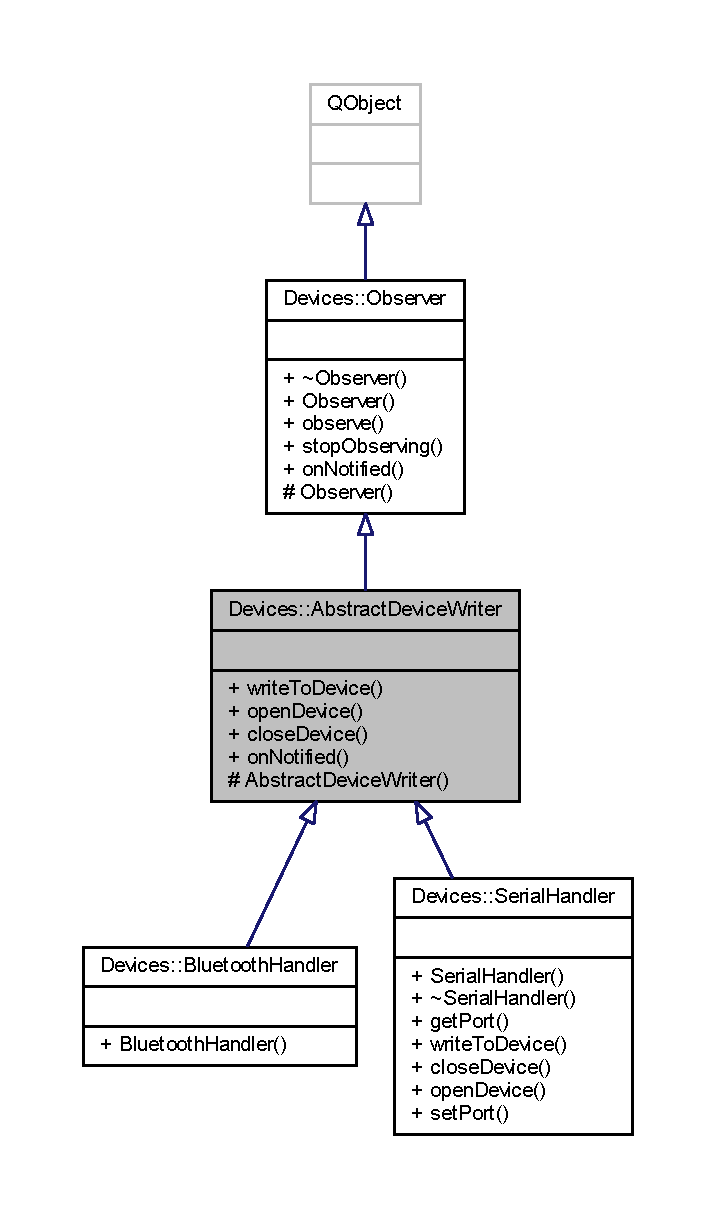
\includegraphics[height=550pt]{d5/d98/class_devices_1_1_abstract_device_writer__inherit__graph}
\end{center}
\end{figure}


Collaboration diagram for Devices\+:\+:Abstract\+Device\+Writer\+:\nopagebreak
\begin{figure}[H]
\begin{center}
\leavevmode
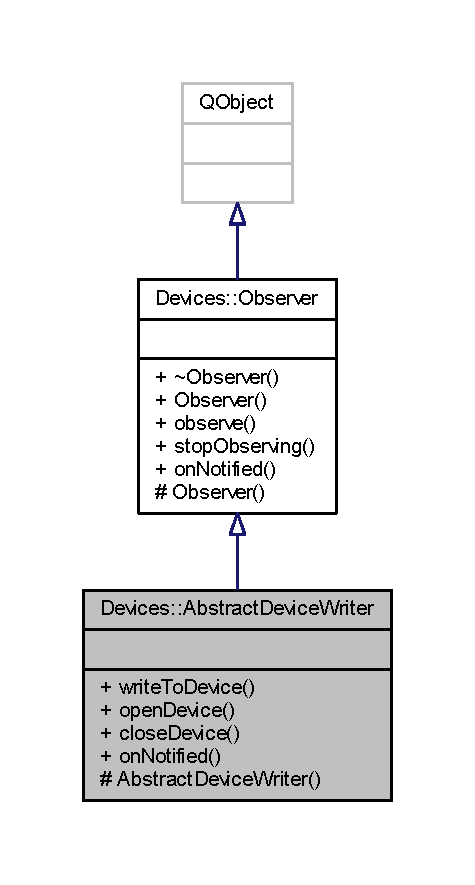
\includegraphics[width=228pt]{d2/dd2/class_devices_1_1_abstract_device_writer__coll__graph}
\end{center}
\end{figure}
\subsection*{Public Slots}
\begin{DoxyCompactItemize}
\item 
\mbox{\Hypertarget{class_devices_1_1_abstract_device_writer_aa492a61c7df1e5588447a1fe4623b2bf}\label{class_devices_1_1_abstract_device_writer_aa492a61c7df1e5588447a1fe4623b2bf}} 
virtual void {\bfseries on\+Notified} (const \hyperlink{class_devices_1_1_observable_data}{Observable\+Data} \&dt) override
\end{DoxyCompactItemize}
\subsection*{Signals}
\begin{DoxyCompactItemize}
\item 
\mbox{\Hypertarget{class_devices_1_1_abstract_device_writer_aa882d8ef6221c76245ee8e5273caae85}\label{class_devices_1_1_abstract_device_writer_aa882d8ef6221c76245ee8e5273caae85}} 
void {\bfseries error\+I\+O\+Device} (const Q\+String \&)
\end{DoxyCompactItemize}
\subsection*{Public Member Functions}
\begin{DoxyCompactItemize}
\item 
\mbox{\Hypertarget{class_devices_1_1_abstract_device_writer_a5fad14b09f0fed1f225e45efa7f19122}\label{class_devices_1_1_abstract_device_writer_a5fad14b09f0fed1f225e45efa7f19122}} 
virtual void {\bfseries write\+To\+Device} (const Q\+String \&)=0
\item 
\mbox{\Hypertarget{class_devices_1_1_abstract_device_writer_ab0b97c22bd53240a29e997b7e665956d}\label{class_devices_1_1_abstract_device_writer_ab0b97c22bd53240a29e997b7e665956d}} 
virtual void {\bfseries open\+Device} ()=0
\item 
\mbox{\Hypertarget{class_devices_1_1_abstract_device_writer_a04ef6838866f61e59eb56bfff11b3da6}\label{class_devices_1_1_abstract_device_writer_a04ef6838866f61e59eb56bfff11b3da6}} 
virtual void {\bfseries close\+Device} ()=0
\end{DoxyCompactItemize}
\subsection*{Protected Member Functions}
\begin{DoxyCompactItemize}
\item 
\mbox{\Hypertarget{class_devices_1_1_abstract_device_writer_a25679076ac5f57cbc317a8c07c1ebf25}\label{class_devices_1_1_abstract_device_writer_a25679076ac5f57cbc317a8c07c1ebf25}} 
{\bfseries Abstract\+Device\+Writer} (Q\+Object $\ast$parent=nullptr)
\end{DoxyCompactItemize}


The documentation for this class was generated from the following files\+:\begin{DoxyCompactItemize}
\item 
src/\+Object\+Detection/\+Devices\+Interfaces/\+Device\+Handler/abstractdevicewriter.\+h\item 
src/\+Object\+Detection/\+Devices\+Interfaces/\+Device\+Handler/abstractdevicewriter.\+cpp\end{DoxyCompactItemize}

\hypertarget{class_image_processor_1_1_abstract_image_processor}{}\section{Image\+Processor\+:\+:Abstract\+Image\+Processor Class Reference}
\label{class_image_processor_1_1_abstract_image_processor}\index{Image\+Processor\+::\+Abstract\+Image\+Processor@{Image\+Processor\+::\+Abstract\+Image\+Processor}}


The \hyperlink{class_image_processor_1_1_abstract_image_processor}{Image\+Processor\+::\+Abstract\+Image\+Processor} is an Abstract Base Class For All Image Processor Classes.  




Inheritance diagram for Image\+Processor\+:\+:Abstract\+Image\+Processor\+:\nopagebreak
\begin{figure}[H]
\begin{center}
\leavevmode
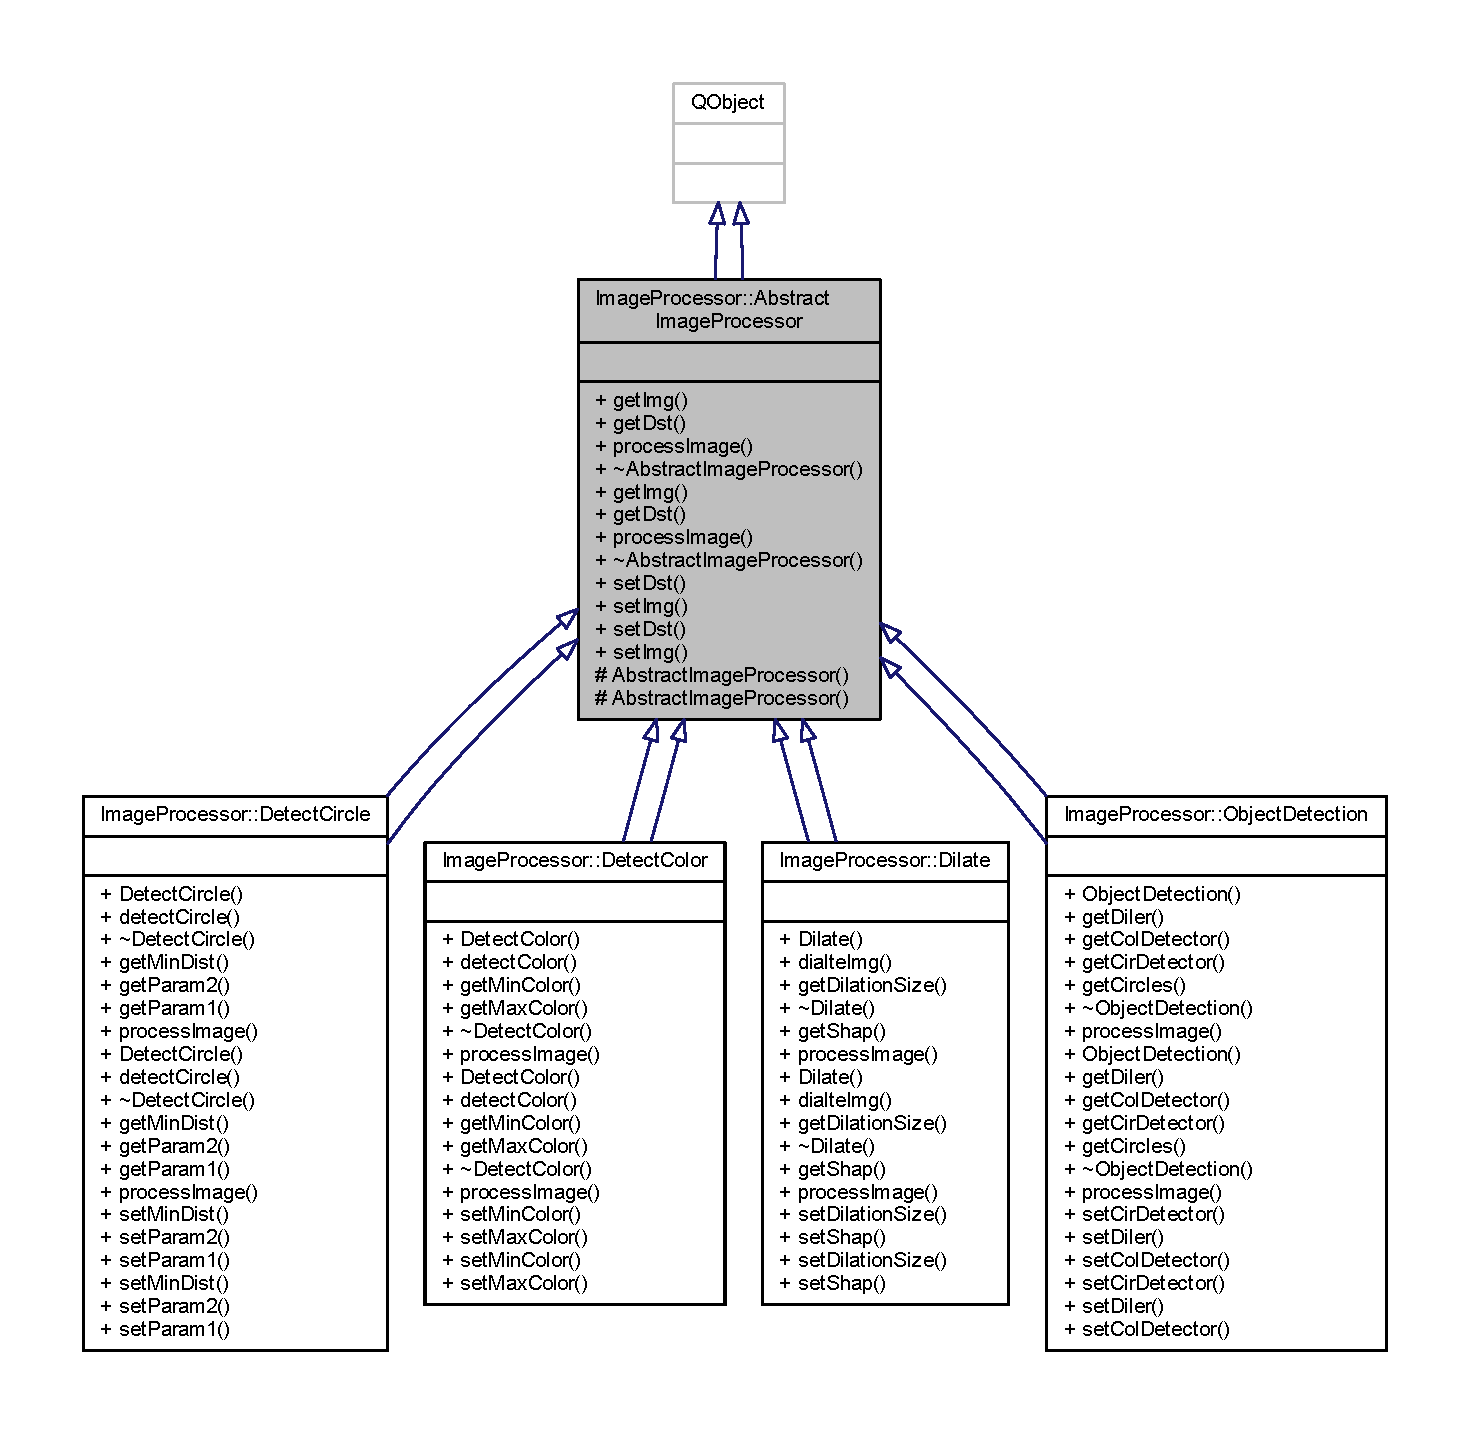
\includegraphics[width=350pt]{d5/d49/class_image_processor_1_1_abstract_image_processor__inherit__graph}
\end{center}
\end{figure}


Collaboration diagram for Image\+Processor\+:\+:Abstract\+Image\+Processor\+:\nopagebreak
\begin{figure}[H]
\begin{center}
\leavevmode
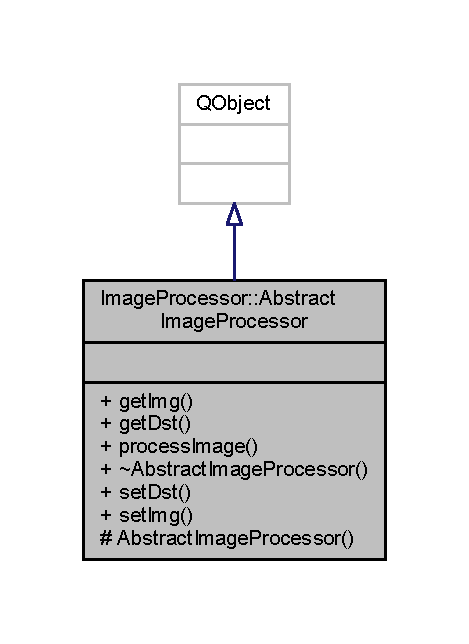
\includegraphics[width=225pt]{d2/d0a/class_image_processor_1_1_abstract_image_processor__coll__graph}
\end{center}
\end{figure}
\subsection*{Classes}
\begin{DoxyCompactItemize}
\item 
class {\bfseries \+\_\+\+Abstract\+Image\+Processor\+Impl}
\end{DoxyCompactItemize}
\subsection*{Public Slots}
\begin{DoxyCompactItemize}
\item 
virtual void \hyperlink{class_image_processor_1_1_abstract_image_processor_a8d9dcbea1b426f4accdd8fcc650eb6ab}{set\+Dst} (const cv\+::\+Mat \&dst)
\begin{DoxyCompactList}\small\item\em sets The output of the operation \end{DoxyCompactList}\item 
\mbox{\Hypertarget{class_image_processor_1_1_abstract_image_processor_a08c1e75c34cb5724e8b3ed4e55d90fb9}\label{class_image_processor_1_1_abstract_image_processor_a08c1e75c34cb5724e8b3ed4e55d90fb9}} 
virtual void {\bfseries set\+Img} (const cv\+::\+Mat \&img)
\item 
\mbox{\Hypertarget{class_image_processor_1_1_abstract_image_processor_ac3cb6442277dc17f1cf2f2215c2cdab2}\label{class_image_processor_1_1_abstract_image_processor_ac3cb6442277dc17f1cf2f2215c2cdab2}} 
virtual void {\bfseries set\+Dst} (const cv\+::\+Mat \&dst)
\item 
\mbox{\Hypertarget{class_image_processor_1_1_abstract_image_processor_a240c3eec8500e5d2432b27a7b68b55b2}\label{class_image_processor_1_1_abstract_image_processor_a240c3eec8500e5d2432b27a7b68b55b2}} 
virtual void {\bfseries set\+Img} (const cv\+::\+Mat \&img)
\end{DoxyCompactItemize}
\subsection*{Signals}
\begin{DoxyCompactItemize}
\item 
\mbox{\Hypertarget{class_image_processor_1_1_abstract_image_processor_a5a252ccaca15ae5609bf490dff410a44}\label{class_image_processor_1_1_abstract_image_processor_a5a252ccaca15ae5609bf490dff410a44}} 
void {\bfseries image\+Changed} (const cv\+::\+Mat \&img)
\item 
\mbox{\Hypertarget{class_image_processor_1_1_abstract_image_processor_a98d198ad26991ee5fa200d8a1a740448}\label{class_image_processor_1_1_abstract_image_processor_a98d198ad26991ee5fa200d8a1a740448}} 
void {\bfseries dst\+Changed} (const cv\+::\+Mat \&img)
\item 
\mbox{\Hypertarget{class_image_processor_1_1_abstract_image_processor_a5a252ccaca15ae5609bf490dff410a44}\label{class_image_processor_1_1_abstract_image_processor_a5a252ccaca15ae5609bf490dff410a44}} 
void {\bfseries image\+Changed} (const cv\+::\+Mat \&img)
\item 
\mbox{\Hypertarget{class_image_processor_1_1_abstract_image_processor_a98d198ad26991ee5fa200d8a1a740448}\label{class_image_processor_1_1_abstract_image_processor_a98d198ad26991ee5fa200d8a1a740448}} 
void {\bfseries dst\+Changed} (const cv\+::\+Mat \&img)
\end{DoxyCompactItemize}
\subsection*{Public Member Functions}
\begin{DoxyCompactItemize}
\item 
cv\+::\+Mat \hyperlink{class_image_processor_1_1_abstract_image_processor_a904d1619b2c6be2c5382469325ca43e3}{get\+Img} () const
\begin{DoxyCompactList}\small\item\em \hyperlink{class_image_processor_1_1_abstract_image_processor_a904d1619b2c6be2c5382469325ca43e3}{Abstract\+Image\+Processor\+::get\+Img}. \end{DoxyCompactList}\item 
cv\+::\+Mat \hyperlink{class_image_processor_1_1_abstract_image_processor_acbf98498ebece7b9f339222097a3429a}{get\+Dst} () const
\begin{DoxyCompactList}\small\item\em returns A cv\+::\+Mat Object which represents the output of the image processing operation \end{DoxyCompactList}\item 
virtual Q\+Variant \hyperlink{class_image_processor_1_1_abstract_image_processor_ad033ae911918b0f6842b7b1d6cdd2b90}{process\+Image} ()=0
\begin{DoxyCompactList}\small\item\em Pure Virtual Function representes the operation to be done on the Image to be processed. \end{DoxyCompactList}\item 
\mbox{\Hypertarget{class_image_processor_1_1_abstract_image_processor_a767ac703d0d95f54ac3cfc1fe223f6b1}\label{class_image_processor_1_1_abstract_image_processor_a767ac703d0d95f54ac3cfc1fe223f6b1}} 
cv\+::\+Mat {\bfseries get\+Img} () const
\item 
\mbox{\Hypertarget{class_image_processor_1_1_abstract_image_processor_aca36f6820247320a27d5ba8ee923a57e}\label{class_image_processor_1_1_abstract_image_processor_aca36f6820247320a27d5ba8ee923a57e}} 
cv\+::\+Mat {\bfseries get\+Dst} () const
\item 
\mbox{\Hypertarget{class_image_processor_1_1_abstract_image_processor_aefc5e0bf8333b94feca18d2b6458d3ab}\label{class_image_processor_1_1_abstract_image_processor_aefc5e0bf8333b94feca18d2b6458d3ab}} 
virtual Q\+Variant {\bfseries process\+Image} ()=0
\end{DoxyCompactItemize}
\subsection*{Protected Member Functions}
\begin{DoxyCompactItemize}
\item 
\hyperlink{class_image_processor_1_1_abstract_image_processor_a5d89a80ba5924d41809a877e4128039a}{Abstract\+Image\+Processor} (Q\+Object $\ast$parent=nullptr)
\begin{DoxyCompactList}\small\item\em accpets A pointer To the Parent Class For The Qt Meta-\/object Model See \href{http://doc.qt.io/qt-5/metaobjects.html}{\tt Qt Meta-\/\+Object} \end{DoxyCompactList}\item 
\mbox{\Hypertarget{class_image_processor_1_1_abstract_image_processor_afed21785fad3fc501ba80714c5f10c0b}\label{class_image_processor_1_1_abstract_image_processor_afed21785fad3fc501ba80714c5f10c0b}} 
{\bfseries Abstract\+Image\+Processor} (Q\+Object $\ast$parent=nullptr)
\end{DoxyCompactItemize}


\subsection{Detailed Description}
The \hyperlink{class_image_processor_1_1_abstract_image_processor}{Image\+Processor\+::\+Abstract\+Image\+Processor} is an Abstract Base Class For All Image Processor Classes. 

this Class Provides A Common Data Structure For All Image Processor Classes That Inherits From It The class Provides cv\+::\+Mat Img Variable Which is used as The Soruce Image and cv\+::\+Mat dst Varaible Which is the Destnation cv\+::\+Mat Object. \begin{DoxyNote}{Note}
using get\+Dst and get\+Img is using deep copy of image to avoid invalid access of member objects.
\end{DoxyNote}

\begin{DoxyCode}
\textcolor{keyword}{using namespace }\hyperlink{namespace_image_processor}{ImageProcessor};
std::unique\_ptr<ImageProcessor::AbstractImageProcessor> imgproc = 
      std::make\_unique<ImageProcessor::DetectColor>(\textcolor{keyword}{this});
imgproc->setImg(cv::imread(IMG\_PATH));
connect(imgproc.get(), &AbstractImageProcessor::dstChanged,[=](\textcolor{keyword}{const} \textcolor{keyword}{auto}& img)\{qDebug() << \textcolor{stringliteral}{"Image Changed"}
      ;\});
imgproc->processImage();
\textcolor{keyword}{auto} img = imgproc->getDst(); \textcolor{comment}{//returns cv::Mat and prints "Image Changed"}
\end{DoxyCode}
 \begin{DoxySeeAlso}{See also}
\hyperlink{namespace_image_processor}{Image\+Processor} 
\end{DoxySeeAlso}
\begin{DoxyRefDesc}{Todo}
\item[\hyperlink{todo__todo000001}{Todo}]add cv\+::\+Mat cache(may be using flyweight pattern) To avoid heavy copy of cv\+::\+Mat obejcts. \end{DoxyRefDesc}


\subsection{Constructor \& Destructor Documentation}
\mbox{\Hypertarget{class_image_processor_1_1_abstract_image_processor_a5d89a80ba5924d41809a877e4128039a}\label{class_image_processor_1_1_abstract_image_processor_a5d89a80ba5924d41809a877e4128039a}} 
\index{Image\+Processor\+::\+Abstract\+Image\+Processor@{Image\+Processor\+::\+Abstract\+Image\+Processor}!Abstract\+Image\+Processor@{Abstract\+Image\+Processor}}
\index{Abstract\+Image\+Processor@{Abstract\+Image\+Processor}!Image\+Processor\+::\+Abstract\+Image\+Processor@{Image\+Processor\+::\+Abstract\+Image\+Processor}}
\subsubsection{\texorpdfstring{Abstract\+Image\+Processor()}{AbstractImageProcessor()}}
{\footnotesize\ttfamily Abstract\+Image\+Processor\+::\+Abstract\+Image\+Processor (\begin{DoxyParamCaption}\item[{Q\+Object $\ast$}]{parent = {\ttfamily nullptr} }\end{DoxyParamCaption})\hspace{0.3cm}{\ttfamily [protected]}}



accpets A pointer To the Parent Class For The Qt Meta-\/object Model See \href{http://doc.qt.io/qt-5/metaobjects.html}{\tt Qt Meta-\/\+Object} 


\begin{DoxyParams}{Parameters}
{\em parent} & A Q\+Object Object as a parent \\
\hline
\end{DoxyParams}
Here is the caller graph for this function\+:\nopagebreak
\begin{figure}[H]
\begin{center}
\leavevmode
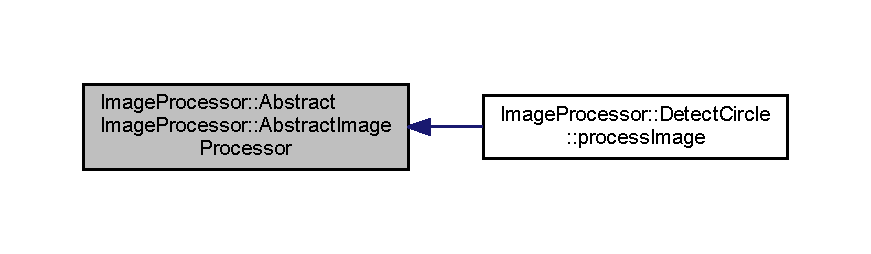
\includegraphics[width=350pt]{dc/d61/class_image_processor_1_1_abstract_image_processor_a5d89a80ba5924d41809a877e4128039a_icgraph}
\end{center}
\end{figure}


\subsection{Member Function Documentation}
\mbox{\Hypertarget{class_image_processor_1_1_abstract_image_processor_acbf98498ebece7b9f339222097a3429a}\label{class_image_processor_1_1_abstract_image_processor_acbf98498ebece7b9f339222097a3429a}} 
\index{Image\+Processor\+::\+Abstract\+Image\+Processor@{Image\+Processor\+::\+Abstract\+Image\+Processor}!get\+Dst@{get\+Dst}}
\index{get\+Dst@{get\+Dst}!Image\+Processor\+::\+Abstract\+Image\+Processor@{Image\+Processor\+::\+Abstract\+Image\+Processor}}
\subsubsection{\texorpdfstring{get\+Dst()}{getDst()}}
{\footnotesize\ttfamily cv\+::\+Mat Abstract\+Image\+Processor\+::get\+Dst (\begin{DoxyParamCaption}{ }\end{DoxyParamCaption}) const}



returns A cv\+::\+Mat Object which represents the output of the image processing operation 

\begin{DoxyReturn}{Returns}
cv\+::\+Mat 
\end{DoxyReturn}
Here is the caller graph for this function\+:\nopagebreak
\begin{figure}[H]
\begin{center}
\leavevmode
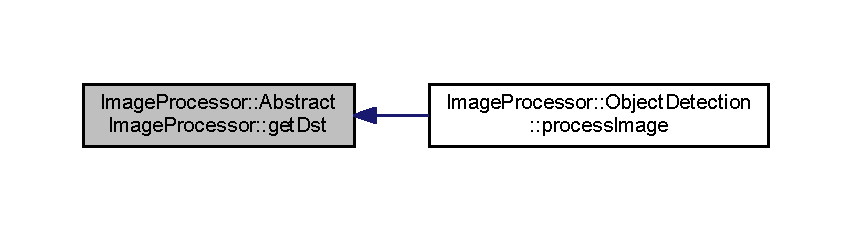
\includegraphics[width=350pt]{dc/d61/class_image_processor_1_1_abstract_image_processor_acbf98498ebece7b9f339222097a3429a_icgraph}
\end{center}
\end{figure}
\mbox{\Hypertarget{class_image_processor_1_1_abstract_image_processor_a904d1619b2c6be2c5382469325ca43e3}\label{class_image_processor_1_1_abstract_image_processor_a904d1619b2c6be2c5382469325ca43e3}} 
\index{Image\+Processor\+::\+Abstract\+Image\+Processor@{Image\+Processor\+::\+Abstract\+Image\+Processor}!get\+Img@{get\+Img}}
\index{get\+Img@{get\+Img}!Image\+Processor\+::\+Abstract\+Image\+Processor@{Image\+Processor\+::\+Abstract\+Image\+Processor}}
\subsubsection{\texorpdfstring{get\+Img()}{getImg()}}
{\footnotesize\ttfamily cv\+::\+Mat Abstract\+Image\+Processor\+::get\+Img (\begin{DoxyParamCaption}{ }\end{DoxyParamCaption}) const}



\hyperlink{class_image_processor_1_1_abstract_image_processor_a904d1619b2c6be2c5382469325ca43e3}{Abstract\+Image\+Processor\+::get\+Img}. 

\begin{DoxyReturn}{Returns}
cv\+::\+Matreturns A copy of The Source Image uses cv\+::\+Mat\+::clone(). {\bfseries example\+:} 
\begin{DoxyCode}
cv::Mat img = cv::imread(IMG\_PATH);
imgproc.setImg(img);
cv::Mat img2 = imgproc.getImg(); \textcolor{comment}{//uses Deep Copy like img2 = img.clone();}
\end{DoxyCode}
 
\end{DoxyReturn}
Here is the caller graph for this function\+:\nopagebreak
\begin{figure}[H]
\begin{center}
\leavevmode
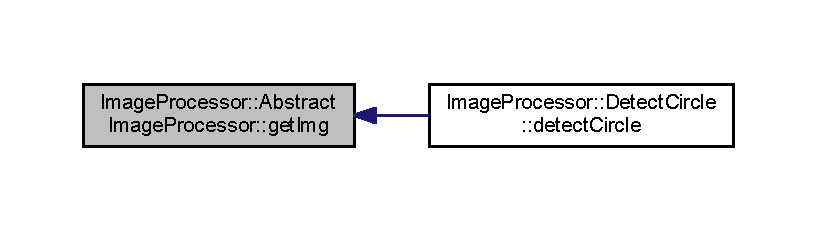
\includegraphics[width=350pt]{dc/d61/class_image_processor_1_1_abstract_image_processor_a904d1619b2c6be2c5382469325ca43e3_icgraph}
\end{center}
\end{figure}
\mbox{\Hypertarget{class_image_processor_1_1_abstract_image_processor_ad033ae911918b0f6842b7b1d6cdd2b90}\label{class_image_processor_1_1_abstract_image_processor_ad033ae911918b0f6842b7b1d6cdd2b90}} 
\index{Image\+Processor\+::\+Abstract\+Image\+Processor@{Image\+Processor\+::\+Abstract\+Image\+Processor}!process\+Image@{process\+Image}}
\index{process\+Image@{process\+Image}!Image\+Processor\+::\+Abstract\+Image\+Processor@{Image\+Processor\+::\+Abstract\+Image\+Processor}}
\subsubsection{\texorpdfstring{process\+Image()}{processImage()}}
{\footnotesize\ttfamily Image\+Processor\+::\+Abstract\+Image\+Processor\+::process\+Image (\begin{DoxyParamCaption}{ }\end{DoxyParamCaption})\hspace{0.3cm}{\ttfamily [pure virtual]}}



Pure Virtual Function representes the operation to be done on the Image to be processed. 


\begin{DoxyExceptions}{Exceptions}
{\em cv\+::\+Exception.\+not} & garunteed to throw this exception \\
\hline
\end{DoxyExceptions}
\begin{DoxyWarning}{Warning}
not exception nor thread safe. 
\end{DoxyWarning}
\begin{DoxyReturn}{Returns}
Q\+Variant Object which represents the output of the processing operation and it doesn\textquotesingle{}t have to be cv\+::\+Mat. 
\end{DoxyReturn}


Implemented in \hyperlink{class_image_processor_1_1_detect_circle_ae0c7b4759827b218a03b16567233b4d5}{Image\+Processor\+::\+Detect\+Circle}, \hyperlink{class_image_processor_1_1_detect_circle_ae59a596ca1e992a8d8f859b5f79239f5}{Image\+Processor\+::\+Detect\+Circle}, \hyperlink{class_image_processor_1_1_object_detection_ac5561650d95eac1672e2d049ed36201d}{Image\+Processor\+::\+Object\+Detection}, \hyperlink{class_image_processor_1_1_object_detection_ad8ff5b55d6da63f30dc397082f97370c}{Image\+Processor\+::\+Object\+Detection}, \hyperlink{class_image_processor_1_1_dilate_ac4af4d83e97990416f1ccc6b80fd140b}{Image\+Processor\+::\+Dilate}, \hyperlink{class_image_processor_1_1_dilate_a47c84e673efe4a1280eede2ea9cb4ef9}{Image\+Processor\+::\+Dilate}, \hyperlink{class_image_processor_1_1_detect_color_afb14622f8e1390f1cf887cc8bf1da568}{Image\+Processor\+::\+Detect\+Color}, and \hyperlink{class_image_processor_1_1_detect_color_a7dc9d23817afafa44a9c022dff64b4a5}{Image\+Processor\+::\+Detect\+Color}.

\mbox{\Hypertarget{class_image_processor_1_1_abstract_image_processor_a8d9dcbea1b426f4accdd8fcc650eb6ab}\label{class_image_processor_1_1_abstract_image_processor_a8d9dcbea1b426f4accdd8fcc650eb6ab}} 
\index{Image\+Processor\+::\+Abstract\+Image\+Processor@{Image\+Processor\+::\+Abstract\+Image\+Processor}!set\+Dst@{set\+Dst}}
\index{set\+Dst@{set\+Dst}!Image\+Processor\+::\+Abstract\+Image\+Processor@{Image\+Processor\+::\+Abstract\+Image\+Processor}}
\subsubsection{\texorpdfstring{set\+Dst}{setDst}}
{\footnotesize\ttfamily void Abstract\+Image\+Processor\+::set\+Dst (\begin{DoxyParamCaption}\item[{const cv\+::\+Mat \&}]{dst }\end{DoxyParamCaption})\hspace{0.3cm}{\ttfamily [virtual]}, {\ttfamily [slot]}}



sets The output of the operation 


\begin{DoxyParams}{Parameters}
{\em dst} & \\
\hline
\end{DoxyParams}


The documentation for this class was generated from the following files\+:\begin{DoxyCompactItemize}
\item 
src/\+Object\+Detection/\+Circle\+Detector/\+Image\+Processors/\+Image\+Processor/abstractimageprocessor.\+h\item 
src/\+Object\+Detection/\+Circle\+Detector/\+Image\+Processors/\+Image\+Processor/abstractimageprocessor.\+cpp\end{DoxyCompactItemize}

\hypertarget{class_devices_1_1_bluetooth_handler}{}\section{Devices\+:\+:Bluetooth\+Handler Class Reference}
\label{class_devices_1_1_bluetooth_handler}\index{Devices\+::\+Bluetooth\+Handler@{Devices\+::\+Bluetooth\+Handler}}


Inheritance diagram for Devices\+:\+:Bluetooth\+Handler\+:\nopagebreak
\begin{figure}[H]
\begin{center}
\leavevmode
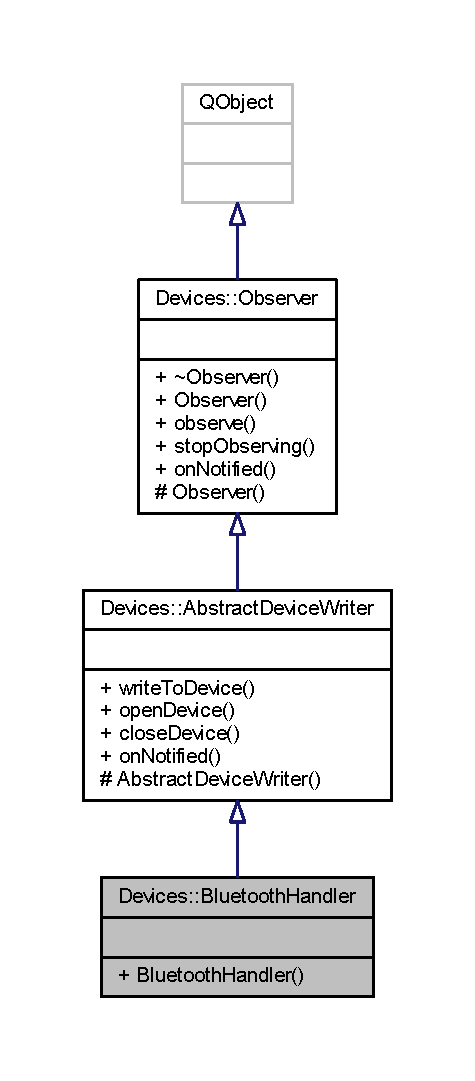
\includegraphics[width=228pt]{d9/d7e/class_devices_1_1_bluetooth_handler__inherit__graph}
\end{center}
\end{figure}


Collaboration diagram for Devices\+:\+:Bluetooth\+Handler\+:\nopagebreak
\begin{figure}[H]
\begin{center}
\leavevmode
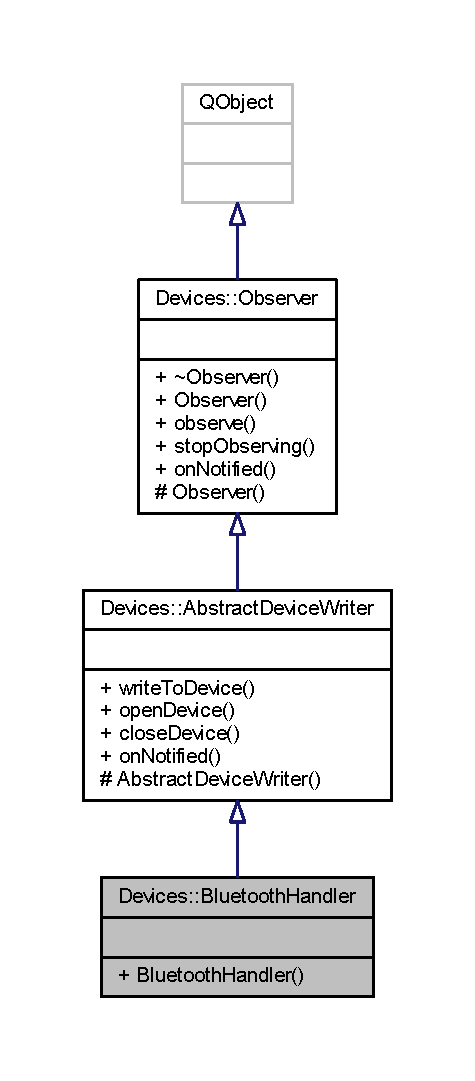
\includegraphics[width=228pt]{dd/ddf/class_devices_1_1_bluetooth_handler__coll__graph}
\end{center}
\end{figure}
\subsection*{Public Member Functions}
\begin{DoxyCompactItemize}
\item 
\mbox{\Hypertarget{class_devices_1_1_bluetooth_handler_ac277c4c65fe0431d33d5875cc3878379}\label{class_devices_1_1_bluetooth_handler_ac277c4c65fe0431d33d5875cc3878379}} 
{\bfseries Bluetooth\+Handler} (Q\+Object $\ast$parent=nullptr)
\end{DoxyCompactItemize}
\subsection*{Additional Inherited Members}


\subsection{Detailed Description}


Definition at line 10 of file bluetoothhandler.\+h.



The documentation for this class was generated from the following files\+:\begin{DoxyCompactItemize}
\item 
object-\/detector/src/\+Devices\+Interfaces/\+Device\+Handler/\+Bluetooth/bluetoothhandler.\+h\item 
object-\/detector/src/\+Devices\+Interfaces/\+Device\+Handler/\+Bluetooth/bluetoothhandler.\+cpp\end{DoxyCompactItemize}

\hypertarget{class_color_detector_controller}{}\section{Color\+Detector\+Controller Class Reference}
\label{class_color_detector_controller}\index{Color\+Detector\+Controller@{Color\+Detector\+Controller}}


Inheritance diagram for Color\+Detector\+Controller\+:\nopagebreak
\begin{figure}[H]
\begin{center}
\leavevmode
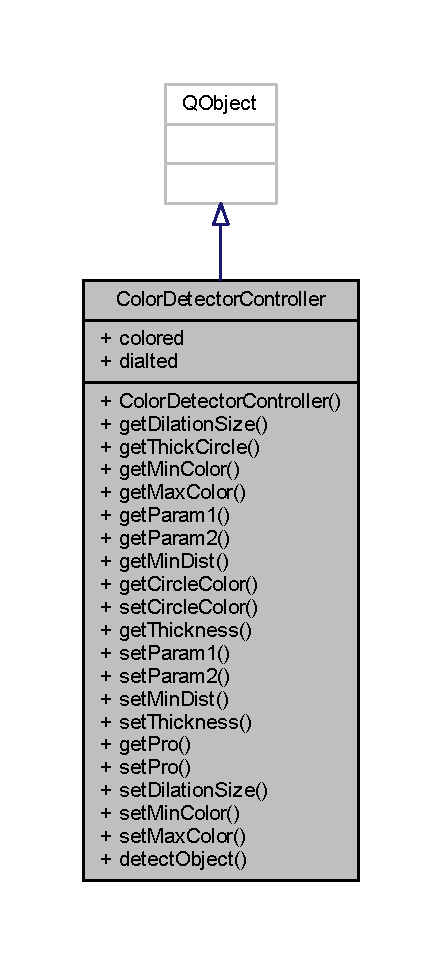
\includegraphics[width=212pt]{d8/d04/class_color_detector_controller__inherit__graph}
\end{center}
\end{figure}


Collaboration diagram for Color\+Detector\+Controller\+:\nopagebreak
\begin{figure}[H]
\begin{center}
\leavevmode
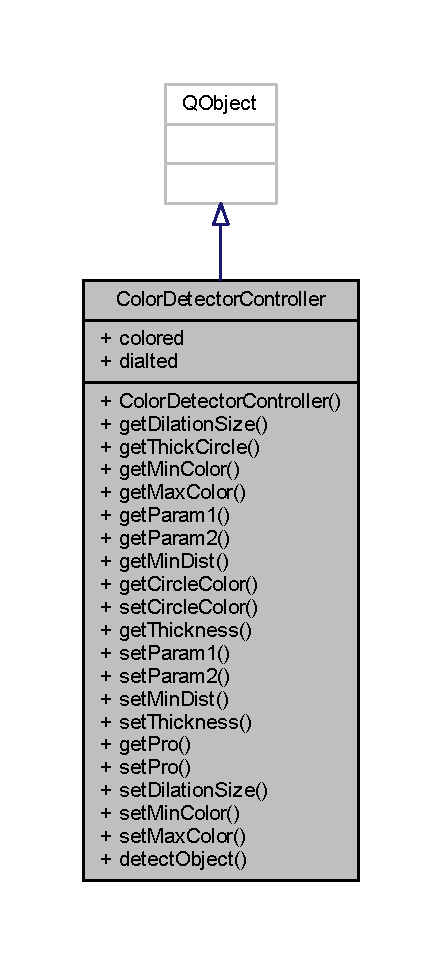
\includegraphics[width=212pt]{d6/d72/class_color_detector_controller__coll__graph}
\end{center}
\end{figure}
\subsection*{Public Slots}
\begin{DoxyCompactItemize}
\item 
\mbox{\Hypertarget{class_color_detector_controller_a12cef009b075aee19592b6f9d5bf4d08}\label{class_color_detector_controller_a12cef009b075aee19592b6f9d5bf4d08}} 
void {\bfseries set\+Param1} (int value)
\item 
\mbox{\Hypertarget{class_color_detector_controller_a3a383fee14bb11464f077843fbef6ef3}\label{class_color_detector_controller_a3a383fee14bb11464f077843fbef6ef3}} 
void {\bfseries set\+Param2} (int value)
\item 
\mbox{\Hypertarget{class_color_detector_controller_aa2d6bc51226ab600bd98a272f4578eea}\label{class_color_detector_controller_aa2d6bc51226ab600bd98a272f4578eea}} 
void {\bfseries set\+Min\+Dist} (int value)
\item 
\mbox{\Hypertarget{class_color_detector_controller_a9e740e8277b4a20331073f06dc21c2b3}\label{class_color_detector_controller_a9e740e8277b4a20331073f06dc21c2b3}} 
void {\bfseries set\+Thickness} (int value)
\item 
\mbox{\Hypertarget{class_color_detector_controller_a2b54a80644a924cbe41c105fc26ecf6f}\label{class_color_detector_controller_a2b54a80644a924cbe41c105fc26ecf6f}} 
void {\bfseries set\+Pro} (\hyperlink{class_image_processor_1_1_object_detection}{Object\+Detection} $\ast$value)
\item 
\mbox{\Hypertarget{class_color_detector_controller_a0f8f5e688e6b6cc636fd9b7b1dd90a0a}\label{class_color_detector_controller_a0f8f5e688e6b6cc636fd9b7b1dd90a0a}} 
void {\bfseries add\+Filter} (Plugin\+Shared\+Pointer filter)
\item 
\mbox{\Hypertarget{class_color_detector_controller_acf885c6d9cc0c81601143d678bb9f890}\label{class_color_detector_controller_acf885c6d9cc0c81601143d678bb9f890}} 
void {\bfseries set\+Dilation\+Size} (int value)
\item 
\mbox{\Hypertarget{class_color_detector_controller_a7bcd481a9b607e2078a68d51158868a7}\label{class_color_detector_controller_a7bcd481a9b607e2078a68d51158868a7}} 
void {\bfseries set\+Min\+Color} (const cv\+::\+Scalar \&value)
\item 
\mbox{\Hypertarget{class_color_detector_controller_ac143c0f40e57336aac8a05f6d6148d12}\label{class_color_detector_controller_ac143c0f40e57336aac8a05f6d6148d12}} 
void {\bfseries set\+Max\+Color} (const cv\+::\+Scalar \&value)
\item 
\mbox{\Hypertarget{class_color_detector_controller_afbf3737d1542b0e1517621b90b7efe15}\label{class_color_detector_controller_afbf3737d1542b0e1517621b90b7efe15}} 
Q\+\_\+\+I\+N\+V\+O\+K\+A\+B\+LE Q\+Image {\bfseries detect\+Object} (const cv\+::\+Mat \&t)
\end{DoxyCompactItemize}
\subsection*{Signals}
\begin{DoxyCompactItemize}
\item 
\mbox{\Hypertarget{class_color_detector_controller_a0750b4604ba5891c67ff470a37477278}\label{class_color_detector_controller_a0750b4604ba5891c67ff470a37477278}} 
void {\bfseries dilation\+Size\+Changed} (int)
\item 
\mbox{\Hypertarget{class_color_detector_controller_af24880bbd700dc3ea4dc876be98c6a06}\label{class_color_detector_controller_af24880bbd700dc3ea4dc876be98c6a06}} 
void {\bfseries min\+Color\+Changed} (const cv\+::\+Scalar \&)
\item 
\mbox{\Hypertarget{class_color_detector_controller_aac5cf8b463491642ae8b85a89b5675d5}\label{class_color_detector_controller_aac5cf8b463491642ae8b85a89b5675d5}} 
void {\bfseries max\+Color\+Changed} (const cv\+::\+Scalar \&)
\item 
\mbox{\Hypertarget{class_color_detector_controller_a9774e7dbb2854b624fa275956aa4b571}\label{class_color_detector_controller_a9774e7dbb2854b624fa275956aa4b571}} 
void {\bfseries param1\+Changed} (int)
\item 
\mbox{\Hypertarget{class_color_detector_controller_a2b8cec0c284d6f24420783f8e11ead88}\label{class_color_detector_controller_a2b8cec0c284d6f24420783f8e11ead88}} 
void {\bfseries param2\+Changed} (int)
\item 
\mbox{\Hypertarget{class_color_detector_controller_ae8f375a29491a3151cb67c6941a3bf6e}\label{class_color_detector_controller_ae8f375a29491a3151cb67c6941a3bf6e}} 
void {\bfseries min\+Dist\+Changed} (int)
\item 
\mbox{\Hypertarget{class_color_detector_controller_a5568479bdc21021dfaad7f61ce82db5d}\label{class_color_detector_controller_a5568479bdc21021dfaad7f61ce82db5d}} 
void {\bfseries xyr\+Changed} (int, int, int)
\end{DoxyCompactItemize}
\subsection*{Public Member Functions}
\begin{DoxyCompactItemize}
\item 
\mbox{\Hypertarget{class_color_detector_controller_a2f35953352a4cba8a1907ca46cf08b62}\label{class_color_detector_controller_a2f35953352a4cba8a1907ca46cf08b62}} 
{\bfseries Color\+Detector\+Controller} (Q\+Object $\ast$parent=nullptr)
\item 
\mbox{\Hypertarget{class_color_detector_controller_afa394dd4972d89f69f06e10bd7992782}\label{class_color_detector_controller_afa394dd4972d89f69f06e10bd7992782}} 
int {\bfseries get\+Dilation\+Size} () const
\item 
\mbox{\Hypertarget{class_color_detector_controller_a7393d5517b607068db7f2ea78484c282}\label{class_color_detector_controller_a7393d5517b607068db7f2ea78484c282}} 
int {\bfseries get\+Thick\+Circle} () const
\item 
\mbox{\Hypertarget{class_color_detector_controller_a8d8b3838562b95f99e17633e3d4c0e12}\label{class_color_detector_controller_a8d8b3838562b95f99e17633e3d4c0e12}} 
cv\+::\+Scalar {\bfseries get\+Min\+Color} () const
\item 
\mbox{\Hypertarget{class_color_detector_controller_a11c07f34537bc17ff113149f94bb9182}\label{class_color_detector_controller_a11c07f34537bc17ff113149f94bb9182}} 
cv\+::\+Scalar {\bfseries get\+Max\+Color} () const
\item 
\mbox{\Hypertarget{class_color_detector_controller_a8cc70b5d53544e5d03ac10b11743c9f5}\label{class_color_detector_controller_a8cc70b5d53544e5d03ac10b11743c9f5}} 
int {\bfseries get\+Param1} () const
\item 
\mbox{\Hypertarget{class_color_detector_controller_a3bea337471bf91256e55c1f729646a32}\label{class_color_detector_controller_a3bea337471bf91256e55c1f729646a32}} 
int {\bfseries get\+Param2} () const
\item 
\mbox{\Hypertarget{class_color_detector_controller_adaf0bc83b6235e0e9997b34ab757f6fd}\label{class_color_detector_controller_adaf0bc83b6235e0e9997b34ab757f6fd}} 
int {\bfseries get\+Min\+Dist} () const
\item 
\mbox{\Hypertarget{class_color_detector_controller_a102cd879ea47cd3143316cd15b752bb0}\label{class_color_detector_controller_a102cd879ea47cd3143316cd15b752bb0}} 
cv\+::\+Scalar {\bfseries get\+Circle\+Color} () const
\item 
\mbox{\Hypertarget{class_color_detector_controller_ac6be48086945d05c1eda3a02b24fd2a9}\label{class_color_detector_controller_ac6be48086945d05c1eda3a02b24fd2a9}} 
void {\bfseries set\+Circle\+Color} (const cv\+::\+Scalar \&value)
\item 
\mbox{\Hypertarget{class_color_detector_controller_a0ca740b6e9e02ad320231c613763f286}\label{class_color_detector_controller_a0ca740b6e9e02ad320231c613763f286}} 
int {\bfseries get\+Thickness} () const
\item 
\mbox{\Hypertarget{class_color_detector_controller_ad1034500aeab80949a9763e9379664db}\label{class_color_detector_controller_ad1034500aeab80949a9763e9379664db}} 
\hyperlink{class_image_processor_1_1_object_detection}{Object\+Detection} $\ast$ {\bfseries get\+Pro} () const
\end{DoxyCompactItemize}
\subsection*{Public Attributes}
\begin{DoxyCompactItemize}
\item 
\mbox{\Hypertarget{class_color_detector_controller_a639034f23f3b7beeaf7001a4a8d5ffd0}\label{class_color_detector_controller_a639034f23f3b7beeaf7001a4a8d5ffd0}} 
cv\+::\+Mat {\bfseries colored}
\item 
\mbox{\Hypertarget{class_color_detector_controller_ab5ae6d433e9192bd1cbd2bb6e95cf675}\label{class_color_detector_controller_ab5ae6d433e9192bd1cbd2bb6e95cf675}} 
cv\+::\+Mat {\bfseries dialted}
\end{DoxyCompactItemize}


\subsection{Detailed Description}


Definition at line 9 of file colordetectorcontroller.\+h.



The documentation for this class was generated from the following files\+:\begin{DoxyCompactItemize}
\item 
object-\/detector/src/\+View/\+Desktop\+View/colordetectorcontroller.\+h\item 
object-\/detector/src/\+View/\+Desktop\+View/colordetectorcontroller.\+cpp\end{DoxyCompactItemize}

\hypertarget{class_image_processor_1_1_detect_circle}{}\section{Image\+Processor\+:\+:Detect\+Circle Class Reference}
\label{class_image_processor_1_1_detect_circle}\index{Image\+Processor\+::\+Detect\+Circle@{Image\+Processor\+::\+Detect\+Circle}}


this class is used To Detect circles in an image  




Inheritance diagram for Image\+Processor\+:\+:Detect\+Circle\+:\nopagebreak
\begin{figure}[H]
\begin{center}
\leavevmode
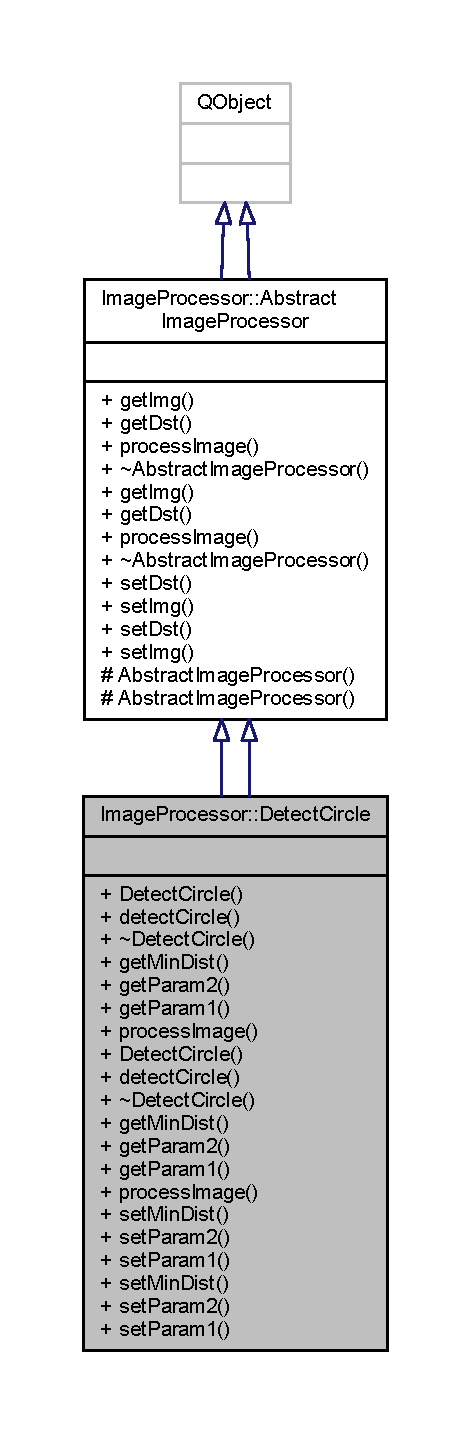
\includegraphics[width=226pt]{de/dd4/class_image_processor_1_1_detect_circle__inherit__graph}
\end{center}
\end{figure}


Collaboration diagram for Image\+Processor\+:\+:Detect\+Circle\+:\nopagebreak
\begin{figure}[H]
\begin{center}
\leavevmode
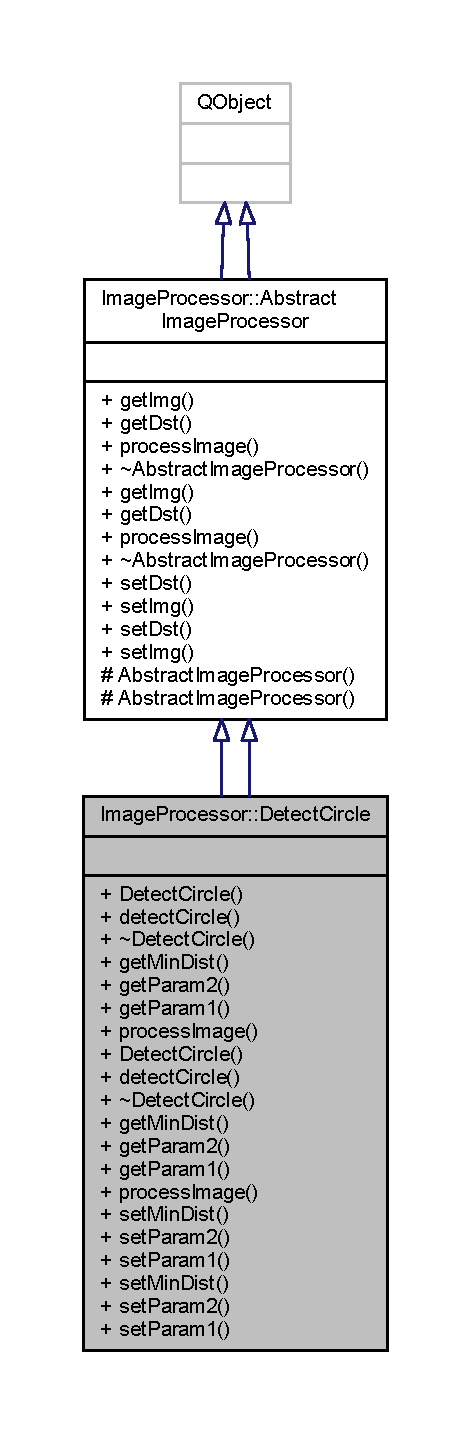
\includegraphics[width=226pt]{d0/d8b/class_image_processor_1_1_detect_circle__coll__graph}
\end{center}
\end{figure}
\subsection*{Classes}
\begin{DoxyCompactItemize}
\item 
class {\bfseries \+\_\+\+Detect\+Circle\+Impl}
\end{DoxyCompactItemize}
\subsection*{Public Slots}
\begin{DoxyCompactItemize}
\item 
void \hyperlink{class_image_processor_1_1_detect_circle_a09bb7bbe753372179b49f94370800021}{set\+Min\+Dist} (int value)
\begin{DoxyCompactList}\small\item\em sets the minimum value between two circles \end{DoxyCompactList}\item 
\mbox{\Hypertarget{class_image_processor_1_1_detect_circle_a6e695fba95e0e6f78620610eee6e00ca}\label{class_image_processor_1_1_detect_circle_a6e695fba95e0e6f78620610eee6e00ca}} 
void {\bfseries set\+Param2} (int value)
\item 
\mbox{\Hypertarget{class_image_processor_1_1_detect_circle_afbc2f237cbac9eb26334953aa5d2b9f0}\label{class_image_processor_1_1_detect_circle_afbc2f237cbac9eb26334953aa5d2b9f0}} 
void {\bfseries set\+Param1} (int value)
\end{DoxyCompactItemize}
\subsection*{Signals}
\begin{DoxyCompactItemize}
\item 
void \hyperlink{class_image_processor_1_1_detect_circle_a2c399b3380a2830317c701d47d4db004}{circles\+Detected} (const std\+::vector$<$ cv\+::\+Vec3f $>$ \&)
\begin{DoxyCompactList}\small\item\em this signal is emitted after detecting All the circles in the image being processed. \end{DoxyCompactList}\end{DoxyCompactItemize}
\subsection*{Public Member Functions}
\begin{DoxyCompactItemize}
\item 
\mbox{\Hypertarget{class_image_processor_1_1_detect_circle_addc37fab154547b0b3b7b7e78bf71d04}\label{class_image_processor_1_1_detect_circle_addc37fab154547b0b3b7b7e78bf71d04}} 
{\bfseries Detect\+Circle} (Q\+Object $\ast$parent=nullptr)
\item 
std\+::vector$<$ cv\+::\+Vec3f $>$ \hyperlink{class_image_processor_1_1_detect_circle_a6324c8bfcc4e8df8d584a037250b22b2}{detect\+Circle} () const
\begin{DoxyCompactList}\small\item\em this helper Function is used to detect circles in an Image using Hough\+Circle Algorithm. \end{DoxyCompactList}\item 
\mbox{\Hypertarget{class_image_processor_1_1_detect_circle_a9e83f089602650f7afcb97172a23f329}\label{class_image_processor_1_1_detect_circle_a9e83f089602650f7afcb97172a23f329}} 
int {\bfseries get\+Min\+Dist} () const
\item 
\mbox{\Hypertarget{class_image_processor_1_1_detect_circle_a8a54460ead0a0204e6321215851d9234}\label{class_image_processor_1_1_detect_circle_a8a54460ead0a0204e6321215851d9234}} 
int {\bfseries get\+Param2} () const
\item 
\mbox{\Hypertarget{class_image_processor_1_1_detect_circle_a4f7719cf36a987db2eb64dc5d8cf0779}\label{class_image_processor_1_1_detect_circle_a4f7719cf36a987db2eb64dc5d8cf0779}} 
int {\bfseries get\+Param1} () const
\item 
Q\+Variant \hyperlink{class_image_processor_1_1_detect_circle_ae0c7b4759827b218a03b16567233b4d5}{process\+Image} () override
\begin{DoxyCompactList}\small\item\em reimplemented Function. \end{DoxyCompactList}\end{DoxyCompactItemize}
\subsection*{Additional Inherited Members}


\subsection{Detailed Description}
this class is used To Detect circles in an image 

using this class you can detect x, y and radius of a circle in an image after calling \hyperlink{class_image_processor_1_1_detect_color_afb14622f8e1390f1cf887cc8bf1da568}{Detect\+Color\+::process\+Image} there are many possible ways to get The output for example you can connect the signal \hyperlink{class_image_processor_1_1_detect_circle_a2c399b3380a2830317c701d47d4db004}{Image\+Processor\+::\+Detect\+Circle\+::circles\+Detected} to any Q\+Object Slot that takes std\+::vector$<$cv\+::\+Vec3f$>$ as a parameter another way is to use the return of process\+Image and convert the Q\+Varient to std\+::vector$<$cv\+::\+Vec3f$>$ 
\begin{DoxyCode}
 connect(crcleDetector, &\hyperlink{class_image_processor_1_1_detect_circle_a2c399b3380a2830317c701d47d4db004}{DetectCircle::circlesDetected}, [=](\textcolor{keyword}{const} 
      std::vector<cv::Vec3f>& vec)\{
     for\_each(vec.begin(), vec.end(), [](cv::Vec3f v)\{ qDebug() << v[0] << \textcolor{stringliteral}{", "} << v[1] << \textcolor{stringliteral}{", "} << v[2];\});
\});
 std::vector<cv::Vec3f> vec = crcleDetector.processImage().value<std::vector<cv::Vec3f>>(); \textcolor{comment}{//and prints
       each x, y, r of every circle.}
\end{DoxyCode}
 \begin{DoxySeeAlso}{See also}
\hyperlink{class_image_processor_1_1_detect_circle_a2c399b3380a2830317c701d47d4db004}{Image\+Processor\+::\+Detect\+Circle\+::circles\+Detected} 
\end{DoxySeeAlso}


Definition at line 12 of file detectcircle.\+h.



\subsection{Member Function Documentation}
\mbox{\Hypertarget{class_image_processor_1_1_detect_circle_a2c399b3380a2830317c701d47d4db004}\label{class_image_processor_1_1_detect_circle_a2c399b3380a2830317c701d47d4db004}} 
\index{Image\+Processor\+::\+Detect\+Circle@{Image\+Processor\+::\+Detect\+Circle}!circles\+Detected@{circles\+Detected}}
\index{circles\+Detected@{circles\+Detected}!Image\+Processor\+::\+Detect\+Circle@{Image\+Processor\+::\+Detect\+Circle}}
\subsubsection{\texorpdfstring{circles\+Detected}{circlesDetected}}
{\footnotesize\ttfamily Image\+Processor\+::\+Detect\+Circle\+::circles\+Detected (\begin{DoxyParamCaption}\item[{const std\+::vector$<$ cv\+::\+Vec3f $>$ \&}]{ }\end{DoxyParamCaption})\hspace{0.3cm}{\ttfamily [signal]}}



this signal is emitted after detecting All the circles in the image being processed. 

can Be connected with other objects to get the circles in an image.


\begin{DoxyCode}
connect(crcleDetector, &\hyperlink{class_image_processor_1_1_detect_circle_a2c399b3380a2830317c701d47d4db004}{DetectCircle::circlesDetected}, [=](\textcolor{keyword}{const} 
      std::vector<cv::Vec3f>& vec)\{
     for\_each(vec.begin(), vec.end(), [](cv::Vec3f v)\{ qDebug() << v[0] << \textcolor{stringliteral}{", "} << v[1] << \textcolor{stringliteral}{", "} << v[2];\});
\}; \textcolor{comment}{//prints each x, y, r of every circle.}
\end{DoxyCode}
 \mbox{\Hypertarget{class_image_processor_1_1_detect_circle_a6324c8bfcc4e8df8d584a037250b22b2}\label{class_image_processor_1_1_detect_circle_a6324c8bfcc4e8df8d584a037250b22b2}} 
\index{Image\+Processor\+::\+Detect\+Circle@{Image\+Processor\+::\+Detect\+Circle}!detect\+Circle@{detect\+Circle}}
\index{detect\+Circle@{detect\+Circle}!Image\+Processor\+::\+Detect\+Circle@{Image\+Processor\+::\+Detect\+Circle}}
\subsubsection{\texorpdfstring{detect\+Circle()}{detectCircle()}}
{\footnotesize\ttfamily std\+::vector$<$ cv\+::\+Vec3f $>$ Detect\+Circle\+::detect\+Circle (\begin{DoxyParamCaption}{ }\end{DoxyParamCaption}) const}



this helper Function is used to detect circles in an Image using Hough\+Circle Algorithm. 

\begin{DoxyReturn}{Returns}
a vector of 3 points vector each represents the x, y, r of all circles in the image. 
\end{DoxyReturn}
\begin{DoxySeeAlso}{See also}
Image\+Processor\+::\+Detect\+Cirlce\+::process\+Image. 
\end{DoxySeeAlso}


Definition at line 66 of file detectcircle.\+cpp.

\mbox{\Hypertarget{class_image_processor_1_1_detect_circle_ae0c7b4759827b218a03b16567233b4d5}\label{class_image_processor_1_1_detect_circle_ae0c7b4759827b218a03b16567233b4d5}} 
\index{Image\+Processor\+::\+Detect\+Circle@{Image\+Processor\+::\+Detect\+Circle}!process\+Image@{process\+Image}}
\index{process\+Image@{process\+Image}!Image\+Processor\+::\+Detect\+Circle@{Image\+Processor\+::\+Detect\+Circle}}
\subsubsection{\texorpdfstring{process\+Image()}{processImage()}}
{\footnotesize\ttfamily Q\+Variant Detect\+Circle\+::process\+Image (\begin{DoxyParamCaption}{ }\end{DoxyParamCaption})\hspace{0.3cm}{\ttfamily [override]}, {\ttfamily [virtual]}}



reimplemented Function. 

this function is reimplented to process a thresholded image of grayscale type to Detect All Cirlces. \begin{DoxySeeAlso}{See also}
\hyperlink{class_image_processor_1_1_abstract_image_processor_ad033ae911918b0f6842b7b1d6cdd2b90}{Image\+Processor\+::\+Abstract\+Image\+Processor\+::process\+Image} 
\end{DoxySeeAlso}
\begin{DoxyReturn}{Returns}
std\+::vector$<$cv\+::\+Vec3f$>$ a vector of cv\+::\+Vec3f where each index in it represents a circle which centers are x, y and radius. 
\begin{DoxyCode}
\textcolor{keyword}{using} circleVec = std::vector<cv::Vec3f>;
\textcolor{keyword}{auto} i = circleDetector.processImage().value<circleVec>();
\textcolor{keywordflow}{for}(\textcolor{keyword}{auto} a : i)\{
     qDebug() << \textcolor{stringliteral}{"x = "} << a[0] << \textcolor{stringliteral}{", y = "} << a[1] << \textcolor{stringliteral}{", r = "} << a[2]; \textcolor{comment}{//should iterate on each element
       and prints it's x, y, and radius.}
\}
\end{DoxyCode}
 
\end{DoxyReturn}


Implements \hyperlink{class_image_processor_1_1_abstract_image_processor_ad033ae911918b0f6842b7b1d6cdd2b90}{Image\+Processor\+::\+Abstract\+Image\+Processor}.



Definition at line 51 of file detectcircle.\+cpp.

Here is the call graph for this function\+:\nopagebreak
\begin{figure}[H]
\begin{center}
\leavevmode
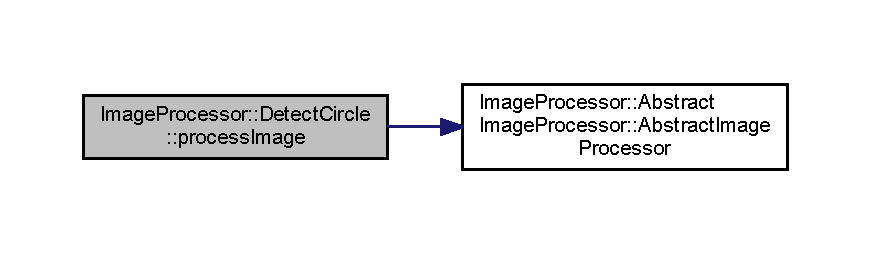
\includegraphics[width=350pt]{d6/d8e/class_image_processor_1_1_detect_circle_ae0c7b4759827b218a03b16567233b4d5_cgraph}
\end{center}
\end{figure}
\mbox{\Hypertarget{class_image_processor_1_1_detect_circle_a09bb7bbe753372179b49f94370800021}\label{class_image_processor_1_1_detect_circle_a09bb7bbe753372179b49f94370800021}} 
\index{Image\+Processor\+::\+Detect\+Circle@{Image\+Processor\+::\+Detect\+Circle}!set\+Min\+Dist@{set\+Min\+Dist}}
\index{set\+Min\+Dist@{set\+Min\+Dist}!Image\+Processor\+::\+Detect\+Circle@{Image\+Processor\+::\+Detect\+Circle}}
\subsubsection{\texorpdfstring{set\+Min\+Dist}{setMinDist}}
{\footnotesize\ttfamily void Detect\+Circle\+::set\+Min\+Dist (\begin{DoxyParamCaption}\item[{int}]{value }\end{DoxyParamCaption})\hspace{0.3cm}{\ttfamily [slot]}}



sets the minimum value between two circles 


\begin{DoxyParams}{Parameters}
{\em value} & \\
\hline
\end{DoxyParams}
\begin{DoxySeeAlso}{See also}
Image\+Processor\+::\+Detect\+Circle\+::get\+Min\+Dist 
\end{DoxySeeAlso}


Definition at line 14 of file detectcircle.\+cpp.



The documentation for this class was generated from the following files\+:\begin{DoxyCompactItemize}
\item 
object-\/detector/src/\+Circle\+Detector/\+Image\+Processors/\+Image\+Processor/detectcircle.\+h\item 
object-\/detector/src/\+Circle\+Detector/\+Image\+Processors/\+Image\+Processor/detectcircle.\+cpp\end{DoxyCompactItemize}

\hypertarget{class_image_processor_1_1_detect_color}{}\section{Image\+Processor\+:\+:Detect\+Color Class Reference}
\label{class_image_processor_1_1_detect_color}\index{Image\+Processor\+::\+Detect\+Color@{Image\+Processor\+::\+Detect\+Color}}


this class is used to Detect Color given it\textquotesingle{}s range(min, max) of hsv colors.  




Inheritance diagram for Image\+Processor\+:\+:Detect\+Color\+:\nopagebreak
\begin{figure}[H]
\begin{center}
\leavevmode
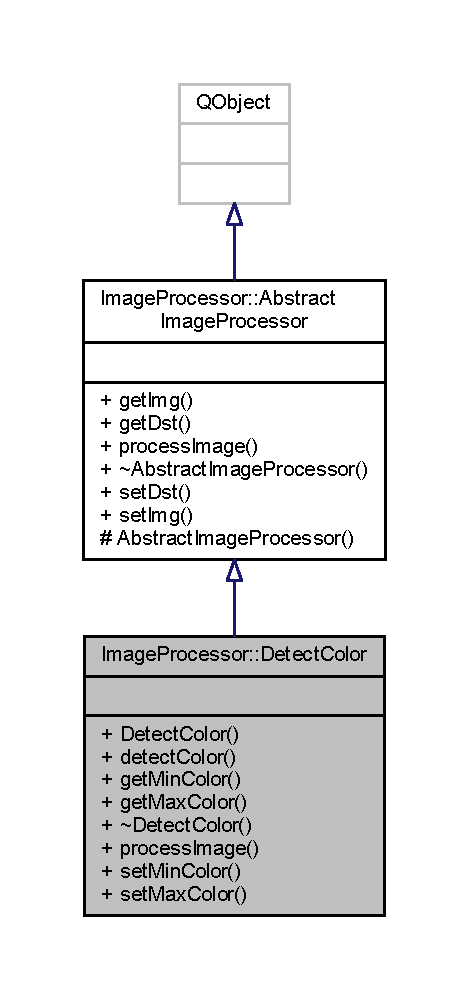
\includegraphics[width=225pt]{d2/d7f/class_image_processor_1_1_detect_color__inherit__graph}
\end{center}
\end{figure}


Collaboration diagram for Image\+Processor\+:\+:Detect\+Color\+:\nopagebreak
\begin{figure}[H]
\begin{center}
\leavevmode
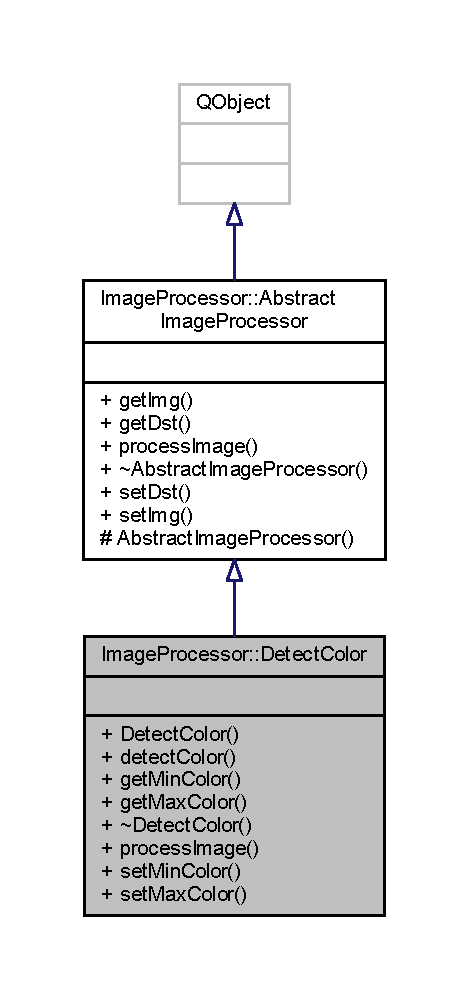
\includegraphics[width=225pt]{d6/dc2/class_image_processor_1_1_detect_color__coll__graph}
\end{center}
\end{figure}
\subsection*{Classes}
\begin{DoxyCompactItemize}
\item 
class {\bfseries \+\_\+\+Detect\+Color\+Impl}
\end{DoxyCompactItemize}
\subsection*{Public Slots}
\begin{DoxyCompactItemize}
\item 
void \hyperlink{class_image_processor_1_1_detect_color_af9f1efdf1535b8a8516c3feb536fc8b8}{set\+Min\+Color} (const cv\+::\+Scalar \&value)
\begin{DoxyCompactList}\small\item\em sets The Minimum hsv color for the Detector \end{DoxyCompactList}\item 
void \hyperlink{class_image_processor_1_1_detect_color_a71bfe53fe223a7342e17e64adf483b84}{set\+Max\+Color} (const cv\+::\+Scalar \&value)
\begin{DoxyCompactList}\small\item\em sets The maximum hsv color for the Detector \end{DoxyCompactList}\end{DoxyCompactItemize}
\subsection*{Public Member Functions}
\begin{DoxyCompactItemize}
\item 
\mbox{\Hypertarget{class_image_processor_1_1_detect_color_a2e6f1c8194a6f98bd9ef1f61c45ca96a}\label{class_image_processor_1_1_detect_color_a2e6f1c8194a6f98bd9ef1f61c45ca96a}} 
{\bfseries Detect\+Color} (Q\+Object $\ast$parent=nullptr)
\item 
void \hyperlink{class_image_processor_1_1_detect_color_a2097eb7955a1f87fa5aa21944197fa17}{detect\+Color} ()
\begin{DoxyCompactList}\small\item\em Helper Function Used To Detect Color. \end{DoxyCompactList}\item 
cv\+::\+Scalar \hyperlink{class_image_processor_1_1_detect_color_a968a764ffc529d9a7022942c047559eb}{get\+Min\+Color} () const
\begin{DoxyCompactList}\small\item\em returns the Minimum H\+SV Color space Of Threshold Detector \end{DoxyCompactList}\item 
cv\+::\+Scalar \hyperlink{class_image_processor_1_1_detect_color_a80a162584cbb4f2ccb452f35bfee19f5}{get\+Max\+Color} () const
\begin{DoxyCompactList}\small\item\em returns the maximum H\+SV Color space Of Threshold Detector \end{DoxyCompactList}\item 
virtual Q\+Variant \hyperlink{class_image_processor_1_1_detect_color_afb14622f8e1390f1cf887cc8bf1da568}{process\+Image} () override
\begin{DoxyCompactList}\small\item\em Pure Virtual Function representes the operation to be done on the Image to be processed. \end{DoxyCompactList}\end{DoxyCompactItemize}
\subsection*{Additional Inherited Members}


\subsection{Detailed Description}
this class is used to Detect Color given it\textquotesingle{}s range(min, max) of hsv colors. 

\begin{DoxyNote}{Note}
Default Color To Detect Is Yellow
\end{DoxyNote}

\begin{DoxyCode}
  cv::Scalar minColor = cv::Scalar(20, 100, 100);
 cv::Scalar  maxColor = cv::Scalar(30, 255, 255); \textcolor{comment}{// detect Yellow Color}
 \hyperlink{class_image_processor_1_1_detect_color}{ImageProcessor::DetectColor} *proc = \textcolor{keyword}{new} DetectColor(\textcolor{keyword}{nullptr});
 proc->\hyperlink{class_image_processor_1_1_detect_color_a71bfe53fe223a7342e17e64adf483b84}{setMaxColor}(maxColor);
proc->\hyperlink{class_image_processor_1_1_detect_color_af9f1efdf1535b8a8516c3feb536fc8b8}{setMinColor}(minColor);
proc->\hyperlink{class_image_processor_1_1_detect_color_afb14622f8e1390f1cf887cc8bf1da568}{processImage}();
\textcolor{keyword}{auto} img = proc->\hyperlink{class_image_processor_1_1_abstract_image_processor_acbf98498ebece7b9f339222097a3429a}{getDst}();
cv::nameWindow(\textcolor{stringliteral}{"window"});
cv::imshow(\textcolor{stringliteral}{"window"}, img);
cv::waitKey(0);
\end{DoxyCode}
 

Definition at line 13 of file detectcolor.\+h.



\subsection{Member Function Documentation}
\mbox{\Hypertarget{class_image_processor_1_1_detect_color_a2097eb7955a1f87fa5aa21944197fa17}\label{class_image_processor_1_1_detect_color_a2097eb7955a1f87fa5aa21944197fa17}} 
\index{Image\+Processor\+::\+Detect\+Color@{Image\+Processor\+::\+Detect\+Color}!detect\+Color@{detect\+Color}}
\index{detect\+Color@{detect\+Color}!Image\+Processor\+::\+Detect\+Color@{Image\+Processor\+::\+Detect\+Color}}
\subsubsection{\texorpdfstring{detect\+Color()}{detectColor()}}
{\footnotesize\ttfamily void Detect\+Color\+::detect\+Color (\begin{DoxyParamCaption}{ }\end{DoxyParamCaption})}



Helper Function Used To Detect Color. 

\begin{DoxyRefDesc}{Todo}
\item[\hyperlink{todo__todo000002}{Todo}]parallize thresholding operationg. \end{DoxyRefDesc}
\begin{DoxyVersion}{Version}
2.\+0 
\end{DoxyVersion}


Definition at line 59 of file detectcolor.\+cpp.

\mbox{\Hypertarget{class_image_processor_1_1_detect_color_a80a162584cbb4f2ccb452f35bfee19f5}\label{class_image_processor_1_1_detect_color_a80a162584cbb4f2ccb452f35bfee19f5}} 
\index{Image\+Processor\+::\+Detect\+Color@{Image\+Processor\+::\+Detect\+Color}!get\+Max\+Color@{get\+Max\+Color}}
\index{get\+Max\+Color@{get\+Max\+Color}!Image\+Processor\+::\+Detect\+Color@{Image\+Processor\+::\+Detect\+Color}}
\subsubsection{\texorpdfstring{get\+Max\+Color()}{getMaxColor()}}
{\footnotesize\ttfamily cv\+::\+Scalar Detect\+Color\+::get\+Max\+Color (\begin{DoxyParamCaption}{ }\end{DoxyParamCaption}) const}



returns the maximum H\+SV Color space Of Threshold Detector 

\begin{DoxyReturn}{Returns}
cv\+::\+Scalar 
\end{DoxyReturn}


Definition at line 29 of file detectcolor.\+cpp.

\mbox{\Hypertarget{class_image_processor_1_1_detect_color_a968a764ffc529d9a7022942c047559eb}\label{class_image_processor_1_1_detect_color_a968a764ffc529d9a7022942c047559eb}} 
\index{Image\+Processor\+::\+Detect\+Color@{Image\+Processor\+::\+Detect\+Color}!get\+Min\+Color@{get\+Min\+Color}}
\index{get\+Min\+Color@{get\+Min\+Color}!Image\+Processor\+::\+Detect\+Color@{Image\+Processor\+::\+Detect\+Color}}
\subsubsection{\texorpdfstring{get\+Min\+Color()}{getMinColor()}}
{\footnotesize\ttfamily cv\+::\+Scalar Detect\+Color\+::get\+Min\+Color (\begin{DoxyParamCaption}{ }\end{DoxyParamCaption}) const}



returns the Minimum H\+SV Color space Of Threshold Detector 

\begin{DoxyReturn}{Returns}
cv\+::\+Scalar 
\end{DoxyReturn}


Definition at line 13 of file detectcolor.\+cpp.

\mbox{\Hypertarget{class_image_processor_1_1_detect_color_afb14622f8e1390f1cf887cc8bf1da568}\label{class_image_processor_1_1_detect_color_afb14622f8e1390f1cf887cc8bf1da568}} 
\index{Image\+Processor\+::\+Detect\+Color@{Image\+Processor\+::\+Detect\+Color}!process\+Image@{process\+Image}}
\index{process\+Image@{process\+Image}!Image\+Processor\+::\+Detect\+Color@{Image\+Processor\+::\+Detect\+Color}}
\subsubsection{\texorpdfstring{process\+Image()}{processImage()}}
{\footnotesize\ttfamily Q\+Variant Detect\+Color\+::process\+Image (\begin{DoxyParamCaption}{ }\end{DoxyParamCaption})\hspace{0.3cm}{\ttfamily [override]}, {\ttfamily [virtual]}}



Pure Virtual Function representes the operation to be done on the Image to be processed. 


\begin{DoxyExceptions}{Exceptions}
{\em cv\+::\+Exception.\+not} & garunteed to throw this exception \\
\hline
\end{DoxyExceptions}
\begin{DoxyWarning}{Warning}
not exception nor thread safe. 
\end{DoxyWarning}
\begin{DoxyReturn}{Returns}
Q\+Variant Object which represents the output of the processing operation and it doesn\textquotesingle{}t have to be cv\+::\+Mat. 
\end{DoxyReturn}


Implements \hyperlink{class_image_processor_1_1_abstract_image_processor_ad033ae911918b0f6842b7b1d6cdd2b90}{Image\+Processor\+::\+Abstract\+Image\+Processor}.



Definition at line 48 of file detectcolor.\+cpp.

\mbox{\Hypertarget{class_image_processor_1_1_detect_color_a71bfe53fe223a7342e17e64adf483b84}\label{class_image_processor_1_1_detect_color_a71bfe53fe223a7342e17e64adf483b84}} 
\index{Image\+Processor\+::\+Detect\+Color@{Image\+Processor\+::\+Detect\+Color}!set\+Max\+Color@{set\+Max\+Color}}
\index{set\+Max\+Color@{set\+Max\+Color}!Image\+Processor\+::\+Detect\+Color@{Image\+Processor\+::\+Detect\+Color}}
\subsubsection{\texorpdfstring{set\+Max\+Color}{setMaxColor}}
{\footnotesize\ttfamily void Detect\+Color\+::set\+Max\+Color (\begin{DoxyParamCaption}\item[{const cv\+::\+Scalar \&}]{value }\end{DoxyParamCaption})\hspace{0.3cm}{\ttfamily [slot]}}



sets The maximum hsv color for the Detector 


\begin{DoxyParams}{Parameters}
{\em cv\+::\+Scalar} & of the H\+SV Color \\
\hline
\end{DoxyParams}


Definition at line 43 of file detectcolor.\+cpp.

\mbox{\Hypertarget{class_image_processor_1_1_detect_color_af9f1efdf1535b8a8516c3feb536fc8b8}\label{class_image_processor_1_1_detect_color_af9f1efdf1535b8a8516c3feb536fc8b8}} 
\index{Image\+Processor\+::\+Detect\+Color@{Image\+Processor\+::\+Detect\+Color}!set\+Min\+Color@{set\+Min\+Color}}
\index{set\+Min\+Color@{set\+Min\+Color}!Image\+Processor\+::\+Detect\+Color@{Image\+Processor\+::\+Detect\+Color}}
\subsubsection{\texorpdfstring{set\+Min\+Color}{setMinColor}}
{\footnotesize\ttfamily void Detect\+Color\+::set\+Min\+Color (\begin{DoxyParamCaption}\item[{const cv\+::\+Scalar \&}]{value }\end{DoxyParamCaption})\hspace{0.3cm}{\ttfamily [slot]}}



sets The Minimum hsv color for the Detector 


\begin{DoxyParams}{Parameters}
{\em cv\+::\+Scalar} & of the H\+SV Color \\
\hline
\end{DoxyParams}


Definition at line 21 of file detectcolor.\+cpp.



The documentation for this class was generated from the following files\+:\begin{DoxyCompactItemize}
\item 
object-\/detector/src/\+Circle\+Detector/\+Image\+Processors/\+Image\+Processor/detectcolor.\+h\item 
object-\/detector/src/\+Circle\+Detector/\+Image\+Processors/\+Image\+Processor/detectcolor.\+cpp\end{DoxyCompactItemize}

\hypertarget{class_devices_1_1_device_manager}{}\section{Devices\+:\+:Device\+Manager Class Reference}
\label{class_devices_1_1_device_manager}\index{Devices\+::\+Device\+Manager@{Devices\+::\+Device\+Manager}}


Inheritance diagram for Devices\+:\+:Device\+Manager\+:\nopagebreak
\begin{figure}[H]
\begin{center}
\leavevmode
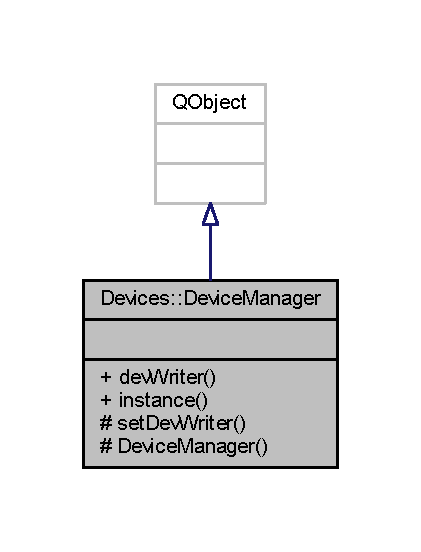
\includegraphics[width=202pt]{dd/daf/class_devices_1_1_device_manager__inherit__graph}
\end{center}
\end{figure}


Collaboration diagram for Devices\+:\+:Device\+Manager\+:\nopagebreak
\begin{figure}[H]
\begin{center}
\leavevmode
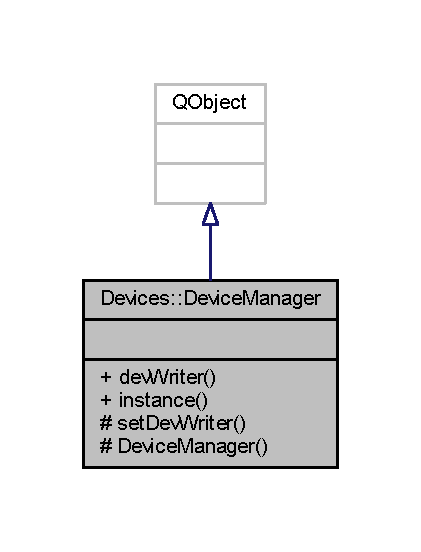
\includegraphics[width=202pt]{d7/dd0/class_devices_1_1_device_manager__coll__graph}
\end{center}
\end{figure}
\subsection*{Public Member Functions}
\begin{DoxyCompactItemize}
\item 
\mbox{\Hypertarget{class_devices_1_1_device_manager_a3d3d30f8dae34a982aa1f5cce1ed49f5}\label{class_devices_1_1_device_manager_a3d3d30f8dae34a982aa1f5cce1ed49f5}} 
\hyperlink{class_devices_1_1_abstract_device_writer}{Devices\+::\+Abstract\+Device\+Writer} $\ast$ {\bfseries dev\+Writer} () const
\end{DoxyCompactItemize}
\subsection*{Static Public Member Functions}
\begin{DoxyCompactItemize}
\item 
\mbox{\Hypertarget{class_devices_1_1_device_manager_ae8d81387e08e66e0f3c1d1d60aa8357f}\label{class_devices_1_1_device_manager_ae8d81387e08e66e0f3c1d1d60aa8357f}} 
static \hyperlink{class_devices_1_1_device_manager}{Device\+Manager} \& {\bfseries instance} (Q\+Object $\ast$parent=nullptr)
\end{DoxyCompactItemize}
\subsection*{Protected Member Functions}
\begin{DoxyCompactItemize}
\item 
\mbox{\Hypertarget{class_devices_1_1_device_manager_a546ce7493ea49bbadf782fa338fd24c4}\label{class_devices_1_1_device_manager_a546ce7493ea49bbadf782fa338fd24c4}} 
void {\bfseries set\+Dev\+Writer} (\hyperlink{class_devices_1_1_abstract_device_writer}{Devices\+::\+Abstract\+Device\+Writer} $\ast$dev\+Writer)
\item 
\mbox{\Hypertarget{class_devices_1_1_device_manager_ae71ec0ba8dac9215cf6c79fb1800e006}\label{class_devices_1_1_device_manager_ae71ec0ba8dac9215cf6c79fb1800e006}} 
{\bfseries Device\+Manager} (Q\+Object $\ast$parent=nullptr)
\end{DoxyCompactItemize}


\subsection{Detailed Description}


Definition at line 12 of file devicemanager.\+h.



The documentation for this class was generated from the following files\+:\begin{DoxyCompactItemize}
\item 
object-\/detector/src/\+Devices\+Interfaces/\+Device\+Handler/devicemanager.\+h\item 
object-\/detector/src/\+Devices\+Interfaces/\+Device\+Handler/devicemanager.\+cpp\end{DoxyCompactItemize}

\hypertarget{class_image_processor_1_1_dilate}{}\section{Image\+Processor\+:\+:Dilate Class Reference}
\label{class_image_processor_1_1_dilate}\index{Image\+Processor\+::\+Dilate@{Image\+Processor\+::\+Dilate}}


this Class is used to perform morphological dilate operation on image see \href{https://docs.opencv.org/trunk/d9/d61/tutorial_py_morphological_ops.html}{\tt Morphological Operation}.  




Inheritance diagram for Image\+Processor\+:\+:Dilate\+:\nopagebreak
\begin{figure}[H]
\begin{center}
\leavevmode
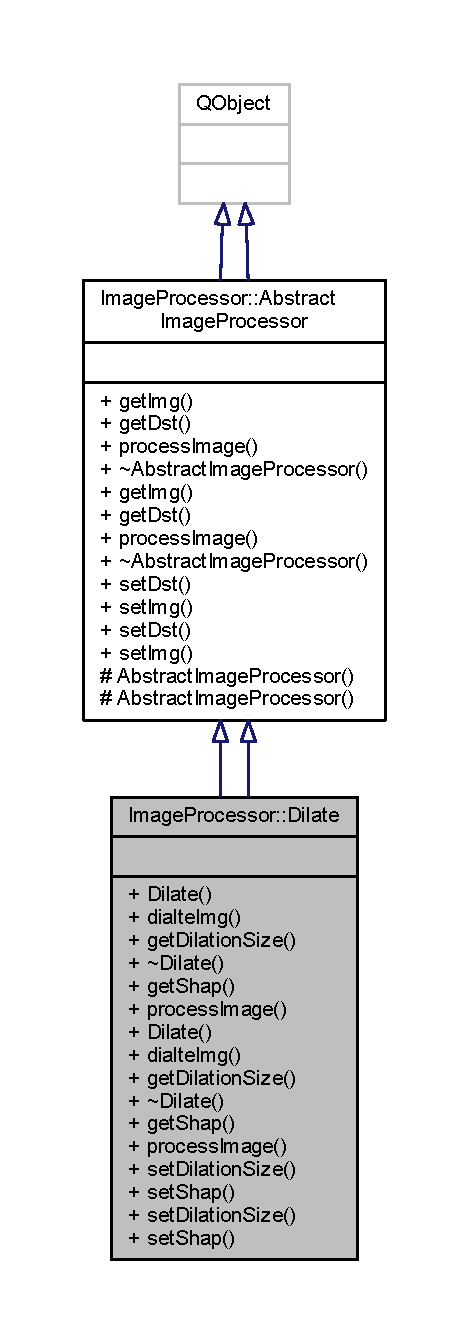
\includegraphics[height=550pt]{dd/d84/class_image_processor_1_1_dilate__inherit__graph}
\end{center}
\end{figure}


Collaboration diagram for Image\+Processor\+:\+:Dilate\+:\nopagebreak
\begin{figure}[H]
\begin{center}
\leavevmode
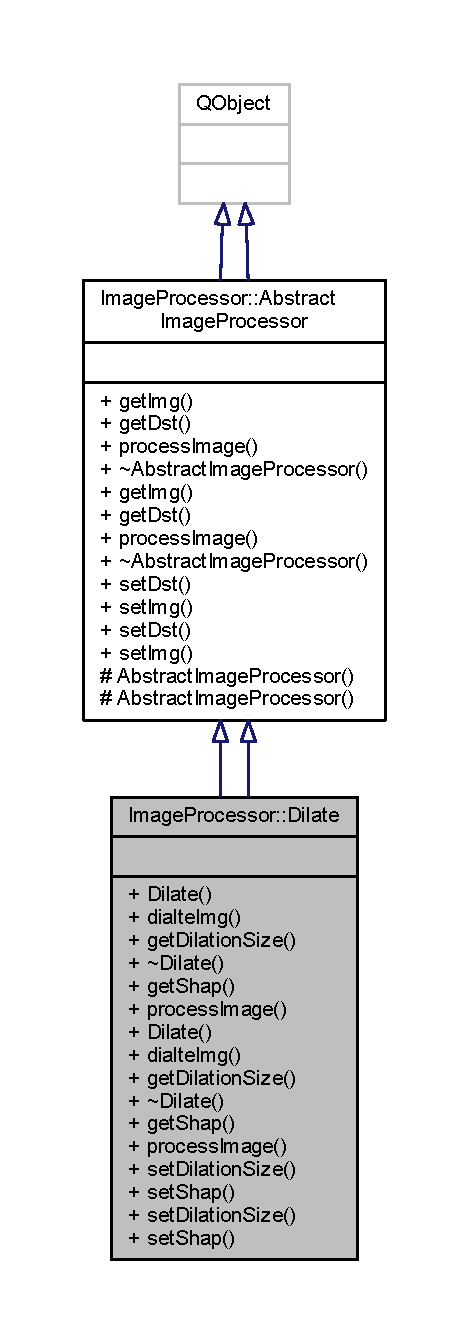
\includegraphics[height=550pt]{d6/d27/class_image_processor_1_1_dilate__coll__graph}
\end{center}
\end{figure}
\subsection*{Classes}
\begin{DoxyCompactItemize}
\item 
class {\bfseries \+\_\+\+Dilate\+Impl}
\end{DoxyCompactItemize}
\subsection*{Public Slots}
\begin{DoxyCompactItemize}
\item 
void \hyperlink{class_image_processor_1_1_dilate_addfbd49b040fc54c9a8985c764f4a144}{set\+Dilation\+Size} (int value)
\begin{DoxyCompactList}\small\item\em sets the Dilation Size of the Morphological Operation \end{DoxyCompactList}\item 
void \hyperlink{class_image_processor_1_1_dilate_a675b54d7fa85c5bce578a625a1f8ec38}{set\+Shap} (const cv\+::\+Morph\+Shapes \&value)
\begin{DoxyCompactList}\small\item\em sets The Shape of the Dialtion pixels \end{DoxyCompactList}\item 
\mbox{\Hypertarget{class_image_processor_1_1_dilate_a38993d0496edc207df78bb98d37e816f}\label{class_image_processor_1_1_dilate_a38993d0496edc207df78bb98d37e816f}} 
void {\bfseries set\+Dilation\+Size} (int value)
\item 
\mbox{\Hypertarget{class_image_processor_1_1_dilate_a244c872bec041a97fc2ef5c7ea89402e}\label{class_image_processor_1_1_dilate_a244c872bec041a97fc2ef5c7ea89402e}} 
void {\bfseries set\+Shap} (const cv\+::\+Morph\+Shapes \&value)
\end{DoxyCompactItemize}
\subsection*{Public Member Functions}
\begin{DoxyCompactItemize}
\item 
\mbox{\Hypertarget{class_image_processor_1_1_dilate_a062fba258056f4e1e1fed226eb05c5f8}\label{class_image_processor_1_1_dilate_a062fba258056f4e1e1fed226eb05c5f8}} 
{\bfseries Dilate} (Q\+Object $\ast$parent=nullptr)
\item 
\mbox{\Hypertarget{class_image_processor_1_1_dilate_aa69a7e5d14912755bd43fdf48f994899}\label{class_image_processor_1_1_dilate_aa69a7e5d14912755bd43fdf48f994899}} 
void {\bfseries dialte\+Img} ()
\item 
int \hyperlink{class_image_processor_1_1_dilate_a52a32329eb187040162c980d72544828}{get\+Dilation\+Size} () const
\begin{DoxyCompactList}\small\item\em returns the dilation Size \end{DoxyCompactList}\item 
\mbox{\Hypertarget{class_image_processor_1_1_dilate_afda6caab7887fecf7e480e8a4ca51773}\label{class_image_processor_1_1_dilate_afda6caab7887fecf7e480e8a4ca51773}} 
cv\+::\+Morph\+Shapes {\bfseries get\+Shap} () const
\item 
virtual Q\+Variant \hyperlink{class_image_processor_1_1_dilate_ac4af4d83e97990416f1ccc6b80fd140b}{process\+Image} () override
\begin{DoxyCompactList}\small\item\em Pure Virtual Function representes the operation to be done on the Image to be processed. \end{DoxyCompactList}\item 
\mbox{\Hypertarget{class_image_processor_1_1_dilate_abf93b190cff3be8559e36f096a2b0db2}\label{class_image_processor_1_1_dilate_abf93b190cff3be8559e36f096a2b0db2}} 
{\bfseries Dilate} (Q\+Object $\ast$parent=nullptr)
\item 
\mbox{\Hypertarget{class_image_processor_1_1_dilate_af999e128e89020d9acd1a07d8ae0e9a8}\label{class_image_processor_1_1_dilate_af999e128e89020d9acd1a07d8ae0e9a8}} 
void {\bfseries dialte\+Img} ()
\item 
\mbox{\Hypertarget{class_image_processor_1_1_dilate_a5f3963a2b176da75fab8fb1a40f38e2e}\label{class_image_processor_1_1_dilate_a5f3963a2b176da75fab8fb1a40f38e2e}} 
int {\bfseries get\+Dilation\+Size} () const
\item 
\mbox{\Hypertarget{class_image_processor_1_1_dilate_a8ead69e76186a999b2d91915399bcfa6}\label{class_image_processor_1_1_dilate_a8ead69e76186a999b2d91915399bcfa6}} 
cv\+::\+Morph\+Shapes {\bfseries get\+Shap} () const
\item 
virtual Q\+Variant \hyperlink{class_image_processor_1_1_dilate_a47c84e673efe4a1280eede2ea9cb4ef9}{process\+Image} () override
\begin{DoxyCompactList}\small\item\em Pure Virtual Function representes the operation to be done on the Image to be processed. \end{DoxyCompactList}\end{DoxyCompactItemize}
\subsection*{Additional Inherited Members}


\subsection{Detailed Description}
this Class is used to perform morphological dilate operation on image see \href{https://docs.opencv.org/trunk/d9/d61/tutorial_py_morphological_ops.html}{\tt Morphological Operation}. 

\begin{DoxyNote}{Note}
the image must be binary (black and white) and in grayscale.
\end{DoxyNote}

\begin{DoxyCode}
 ImageProcessor::Dialte dial\{\textcolor{keyword}{this}\};
dial.setImg(cv::imread(BINARY\_IMG\_PATH));
dial.processImage();
\textcolor{keyword}{auto} dst = dial.getDst();
cv::imshow(\textcolor{stringliteral}{"window"}, dst);
cv::waitKey(0);
\end{DoxyCode}


\begin{DoxyRefDesc}{Todo}
\item[\hyperlink{todo__todo000003}{Todo}]add Other Morphological Operations like erode. \end{DoxyRefDesc}


\subsection{Member Function Documentation}
\mbox{\Hypertarget{class_image_processor_1_1_dilate_a52a32329eb187040162c980d72544828}\label{class_image_processor_1_1_dilate_a52a32329eb187040162c980d72544828}} 
\index{Image\+Processor\+::\+Dilate@{Image\+Processor\+::\+Dilate}!get\+Dilation\+Size@{get\+Dilation\+Size}}
\index{get\+Dilation\+Size@{get\+Dilation\+Size}!Image\+Processor\+::\+Dilate@{Image\+Processor\+::\+Dilate}}
\subsubsection{\texorpdfstring{get\+Dilation\+Size()}{getDilationSize()}}
{\footnotesize\ttfamily int Dilate\+::get\+Dilation\+Size (\begin{DoxyParamCaption}{ }\end{DoxyParamCaption}) const}



returns the dilation Size 

\begin{DoxyReturn}{Returns}

\end{DoxyReturn}
\mbox{\Hypertarget{class_image_processor_1_1_dilate_a47c84e673efe4a1280eede2ea9cb4ef9}\label{class_image_processor_1_1_dilate_a47c84e673efe4a1280eede2ea9cb4ef9}} 
\index{Image\+Processor\+::\+Dilate@{Image\+Processor\+::\+Dilate}!process\+Image@{process\+Image}}
\index{process\+Image@{process\+Image}!Image\+Processor\+::\+Dilate@{Image\+Processor\+::\+Dilate}}
\subsubsection{\texorpdfstring{process\+Image()}{processImage()}\hspace{0.1cm}{\footnotesize\ttfamily [1/2]}}
{\footnotesize\ttfamily virtual Q\+Variant Image\+Processor\+::\+Dilate\+::process\+Image (\begin{DoxyParamCaption}{ }\end{DoxyParamCaption})\hspace{0.3cm}{\ttfamily [override]}, {\ttfamily [virtual]}}



Pure Virtual Function representes the operation to be done on the Image to be processed. 


\begin{DoxyExceptions}{Exceptions}
{\em cv\+::\+Exception.\+not} & garunteed to throw this exception \\
\hline
\end{DoxyExceptions}
\begin{DoxyWarning}{Warning}
not exception nor thread safe. 
\end{DoxyWarning}
\begin{DoxyReturn}{Returns}
Q\+Variant Object which represents the output of the processing operation and it doesn\textquotesingle{}t have to be cv\+::\+Mat. 
\end{DoxyReturn}


Implements \hyperlink{class_image_processor_1_1_abstract_image_processor_ad033ae911918b0f6842b7b1d6cdd2b90}{Image\+Processor\+::\+Abstract\+Image\+Processor}.

\mbox{\Hypertarget{class_image_processor_1_1_dilate_ac4af4d83e97990416f1ccc6b80fd140b}\label{class_image_processor_1_1_dilate_ac4af4d83e97990416f1ccc6b80fd140b}} 
\index{Image\+Processor\+::\+Dilate@{Image\+Processor\+::\+Dilate}!process\+Image@{process\+Image}}
\index{process\+Image@{process\+Image}!Image\+Processor\+::\+Dilate@{Image\+Processor\+::\+Dilate}}
\subsubsection{\texorpdfstring{process\+Image()}{processImage()}\hspace{0.1cm}{\footnotesize\ttfamily [2/2]}}
{\footnotesize\ttfamily Q\+Variant Dilate\+::process\+Image (\begin{DoxyParamCaption}{ }\end{DoxyParamCaption})\hspace{0.3cm}{\ttfamily [override]}, {\ttfamily [virtual]}}



Pure Virtual Function representes the operation to be done on the Image to be processed. 


\begin{DoxyExceptions}{Exceptions}
{\em cv\+::\+Exception.\+not} & garunteed to throw this exception \\
\hline
\end{DoxyExceptions}
\begin{DoxyWarning}{Warning}
not exception nor thread safe. 
\end{DoxyWarning}
\begin{DoxyReturn}{Returns}
Q\+Variant Object which represents the output of the processing operation and it doesn\textquotesingle{}t have to be cv\+::\+Mat. 
\end{DoxyReturn}


Implements \hyperlink{class_image_processor_1_1_abstract_image_processor_ad033ae911918b0f6842b7b1d6cdd2b90}{Image\+Processor\+::\+Abstract\+Image\+Processor}.

\mbox{\Hypertarget{class_image_processor_1_1_dilate_addfbd49b040fc54c9a8985c764f4a144}\label{class_image_processor_1_1_dilate_addfbd49b040fc54c9a8985c764f4a144}} 
\index{Image\+Processor\+::\+Dilate@{Image\+Processor\+::\+Dilate}!set\+Dilation\+Size@{set\+Dilation\+Size}}
\index{set\+Dilation\+Size@{set\+Dilation\+Size}!Image\+Processor\+::\+Dilate@{Image\+Processor\+::\+Dilate}}
\subsubsection{\texorpdfstring{set\+Dilation\+Size}{setDilationSize}}
{\footnotesize\ttfamily void Dilate\+::set\+Dilation\+Size (\begin{DoxyParamCaption}\item[{int}]{value }\end{DoxyParamCaption})\hspace{0.3cm}{\ttfamily [slot]}}



sets the Dilation Size of the Morphological Operation 

\mbox{\Hypertarget{class_image_processor_1_1_dilate_a675b54d7fa85c5bce578a625a1f8ec38}\label{class_image_processor_1_1_dilate_a675b54d7fa85c5bce578a625a1f8ec38}} 
\index{Image\+Processor\+::\+Dilate@{Image\+Processor\+::\+Dilate}!set\+Shap@{set\+Shap}}
\index{set\+Shap@{set\+Shap}!Image\+Processor\+::\+Dilate@{Image\+Processor\+::\+Dilate}}
\subsubsection{\texorpdfstring{set\+Shap}{setShap}}
{\footnotesize\ttfamily void Dilate\+::set\+Shap (\begin{DoxyParamCaption}\item[{const cv\+::\+Morph\+Shapes \&}]{value }\end{DoxyParamCaption})\hspace{0.3cm}{\ttfamily [slot]}}



sets The Shape of the Dialtion pixels 


\begin{DoxyParams}{Parameters}
{\em enum} & of cv\+::\+Morph\+Shapes. \\
\hline
\end{DoxyParams}
\begin{DoxySeeAlso}{See also}
\hyperlink{class_image_processor_1_1_dilate}{Image\+Processor\+::\+Dilate}. 
\end{DoxySeeAlso}


The documentation for this class was generated from the following files\+:\begin{DoxyCompactItemize}
\item 
src/\+Object\+Detection/\+Circle\+Detector/\+Image\+Processors/\+Image\+Processor/dilate.\+h\item 
src/\+Object\+Detection/\+Circle\+Detector/\+Image\+Processors/\+Image\+Processor/dilate.\+cpp\end{DoxyCompactItemize}

\hypertarget{class_image_processor_test}{}\section{Image\+Processor\+Test Class Reference}
\label{class_image_processor_test}\index{Image\+Processor\+Test@{Image\+Processor\+Test}}


Inheritance diagram for Image\+Processor\+Test\+:\nopagebreak
\begin{figure}[H]
\begin{center}
\leavevmode
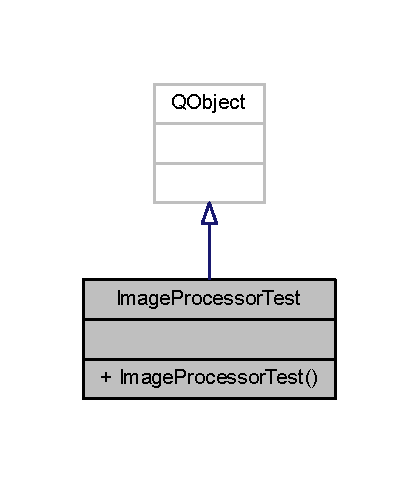
\includegraphics[width=201pt]{d9/dbb/class_image_processor_test__inherit__graph}
\end{center}
\end{figure}


Collaboration diagram for Image\+Processor\+Test\+:\nopagebreak
\begin{figure}[H]
\begin{center}
\leavevmode
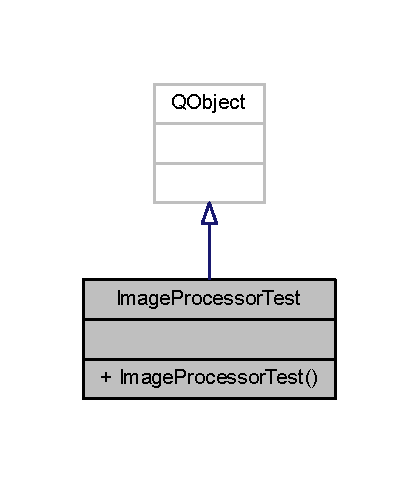
\includegraphics[width=201pt]{d4/d1e/class_image_processor_test__coll__graph}
\end{center}
\end{figure}


\subsection{Detailed Description}


Definition at line 8 of file tst\+\_\+imageprocessortest.\+cpp.



The documentation for this class was generated from the following file\+:\begin{DoxyCompactItemize}
\item 
object-\/detector/src/\+Circle\+Detector/\+Tests/\+Image\+Processor\+Test/tst\+\_\+imageprocessortest.\+cpp\end{DoxyCompactItemize}

\hypertarget{class_main_window}{}\section{Main\+Window Class Reference}
\label{class_main_window}\index{Main\+Window@{Main\+Window}}


Inheritance diagram for Main\+Window\+:\nopagebreak
\begin{figure}[H]
\begin{center}
\leavevmode
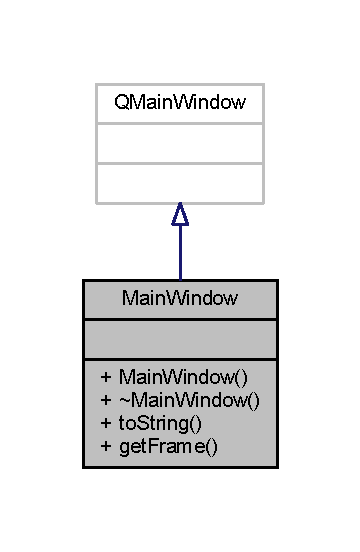
\includegraphics[width=173pt]{de/d4b/class_main_window__inherit__graph}
\end{center}
\end{figure}


Collaboration diagram for Main\+Window\+:\nopagebreak
\begin{figure}[H]
\begin{center}
\leavevmode
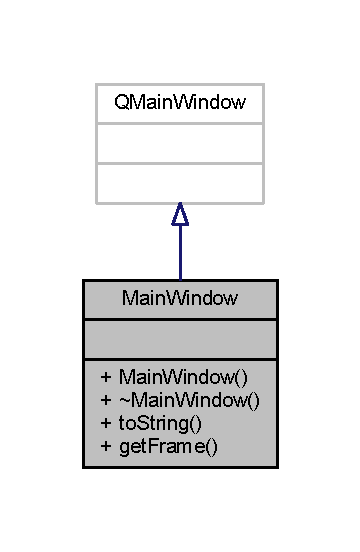
\includegraphics[width=173pt]{d0/db8/class_main_window__coll__graph}
\end{center}
\end{figure}
\subsection*{Public Slots}
\begin{DoxyCompactItemize}
\item 
\mbox{\Hypertarget{class_main_window_a3fdb5e558e83b1e3b45d73544c2488a3}\label{class_main_window_a3fdb5e558e83b1e3b45d73544c2488a3}} 
void {\bfseries get\+Frame} ()
\end{DoxyCompactItemize}
\subsection*{Public Member Functions}
\begin{DoxyCompactItemize}
\item 
\mbox{\Hypertarget{class_main_window_a8b244be8b7b7db1b08de2a2acb9409db}\label{class_main_window_a8b244be8b7b7db1b08de2a2acb9409db}} 
{\bfseries Main\+Window} (Q\+Widget $\ast$parent=0)
\item 
\mbox{\Hypertarget{class_main_window_a2b4d41b838e4fb53f4fdf4951cc69db4}\label{class_main_window_a2b4d41b838e4fb53f4fdf4951cc69db4}} 
Q\+String {\bfseries to\+String} (int x)
\end{DoxyCompactItemize}


The documentation for this class was generated from the following files\+:\begin{DoxyCompactItemize}
\item 
src/\+Object\+Detection/\+View/\+Desktop\+View/\+View/mainwindow.\+h\item 
src/\+Object\+Detection/\+View/\+Desktop\+View/\+View/mainwindow.\+cpp\end{DoxyCompactItemize}

\hypertarget{class_ui_1_1_main_window}{}\section{Ui\+:\+:Main\+Window Class Reference}
\label{class_ui_1_1_main_window}\index{Ui\+::\+Main\+Window@{Ui\+::\+Main\+Window}}


Inheritance diagram for Ui\+:\+:Main\+Window\+:\nopagebreak
\begin{figure}[H]
\begin{center}
\leavevmode
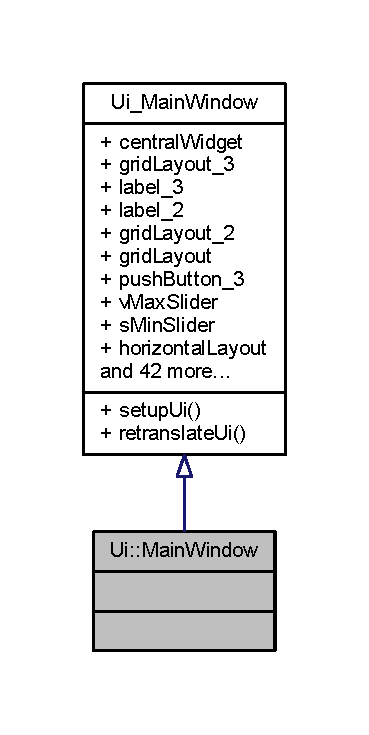
\includegraphics[width=177pt]{d4/de8/class_ui_1_1_main_window__inherit__graph}
\end{center}
\end{figure}


Collaboration diagram for Ui\+:\+:Main\+Window\+:\nopagebreak
\begin{figure}[H]
\begin{center}
\leavevmode
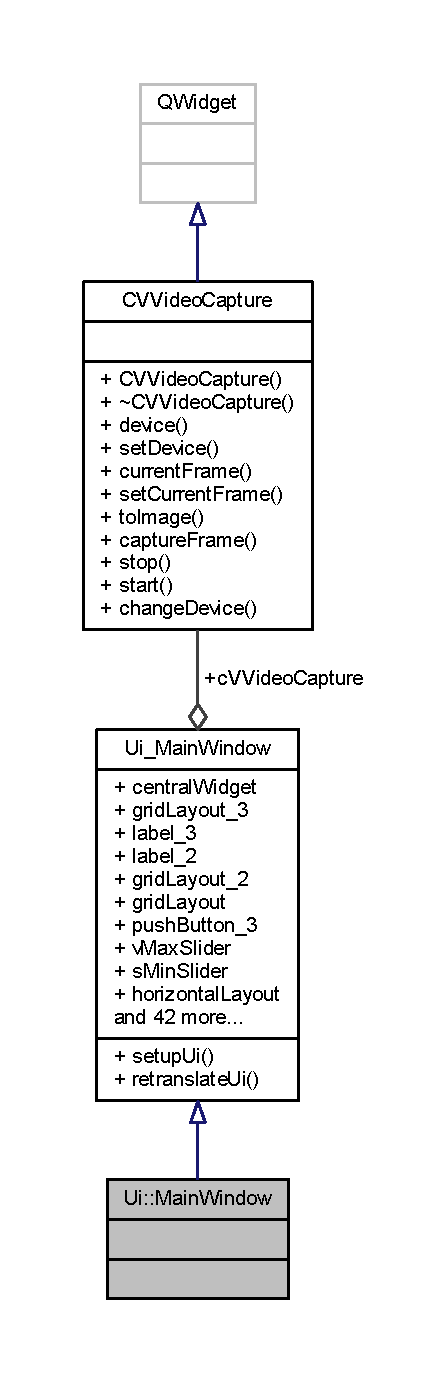
\includegraphics[height=550pt]{dd/dc3/class_ui_1_1_main_window__coll__graph}
\end{center}
\end{figure}
\subsection*{Additional Inherited Members}


\subsection{Detailed Description}


Definition at line 439 of file ui\+\_\+mainwindow.\+h.



The documentation for this class was generated from the following file\+:\begin{DoxyCompactItemize}
\item 
object-\/detector/src/\+View/\+Desktop\+View/\+View/ui\+\_\+mainwindow.\+h\end{DoxyCompactItemize}

\hypertarget{class_image_processor_1_1_object_detection}{}\section{Image\+Processor\+:\+:Object\+Detection Class Reference}
\label{class_image_processor_1_1_object_detection}\index{Image\+Processor\+::\+Object\+Detection@{Image\+Processor\+::\+Object\+Detection}}


this class is used to detect a a colored circle object(s)  




Inheritance diagram for Image\+Processor\+:\+:Object\+Detection\+:\nopagebreak
\begin{figure}[H]
\begin{center}
\leavevmode
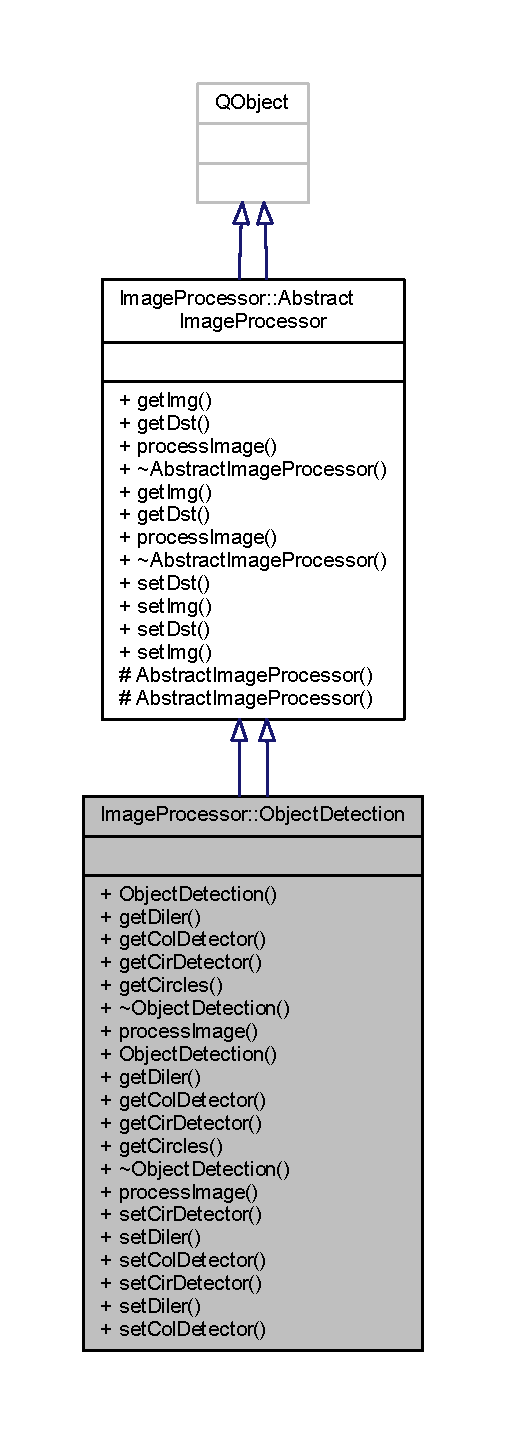
\includegraphics[height=550pt]{da/d04/class_image_processor_1_1_object_detection__inherit__graph}
\end{center}
\end{figure}


Collaboration diagram for Image\+Processor\+:\+:Object\+Detection\+:\nopagebreak
\begin{figure}[H]
\begin{center}
\leavevmode
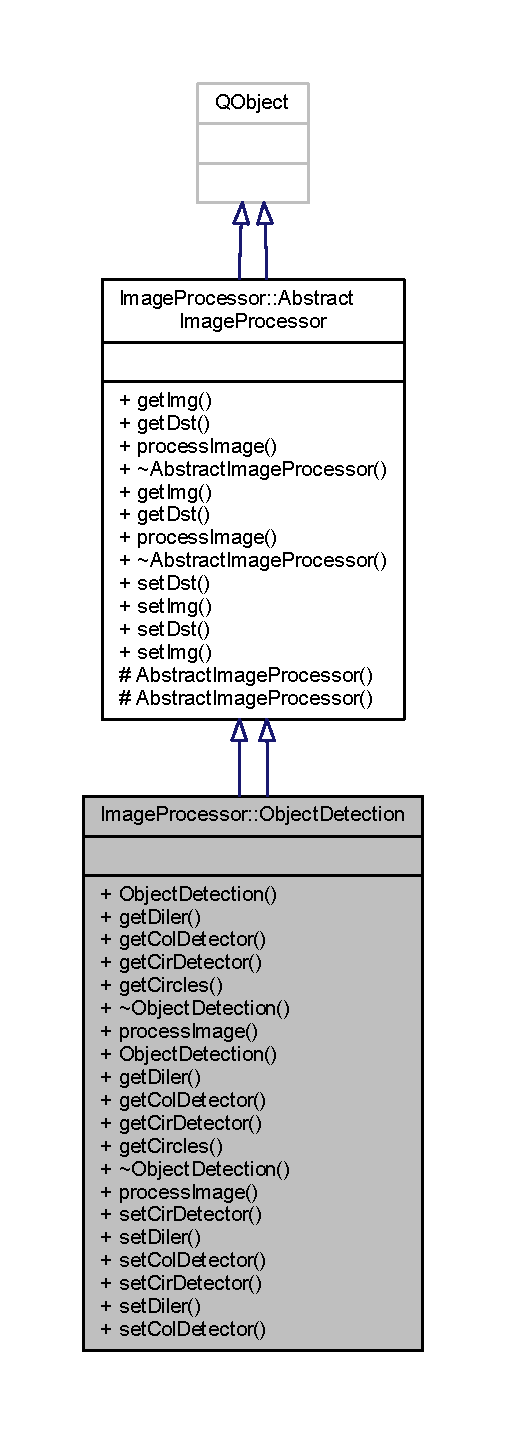
\includegraphics[height=550pt]{d8/daa/class_image_processor_1_1_object_detection__coll__graph}
\end{center}
\end{figure}
\subsection*{Classes}
\begin{DoxyCompactItemize}
\item 
class {\bfseries \+\_\+\+Object\+Detection\+Impl}
\end{DoxyCompactItemize}
\subsection*{Public Slots}
\begin{DoxyCompactItemize}
\item 
void \hyperlink{class_image_processor_1_1_object_detection_afb439c3f4c9bb2e084674ce34e965430}{set\+Cir\+Detector} (\hyperlink{class_image_processor_1_1_detect_circle}{Detect\+Circle} $\ast$cir\+Detector)
\begin{DoxyCompactList}\small\item\em \hyperlink{class_image_processor_1_1_object_detection_afb439c3f4c9bb2e084674ce34e965430}{Object\+Detection\+::set\+Cir\+Detector} sets the circle\+Detector. \end{DoxyCompactList}\item 
void \hyperlink{class_image_processor_1_1_object_detection_a727fcf4d318c9a3ccb63348b957c1e94}{set\+Diler} (\hyperlink{class_image_processor_1_1_dilate}{Dilate} $\ast$diler)
\begin{DoxyCompactList}\small\item\em \hyperlink{class_image_processor_1_1_object_detection_a727fcf4d318c9a3ccb63348b957c1e94}{Object\+Detection\+::set\+Diler} sets the dilate object. \end{DoxyCompactList}\item 
\mbox{\Hypertarget{class_image_processor_1_1_object_detection_abb46bcf3c33130babf9508cb34b08bdf}\label{class_image_processor_1_1_object_detection_abb46bcf3c33130babf9508cb34b08bdf}} 
void {\bfseries set\+Col\+Detector} (\hyperlink{class_image_processor_1_1_detect_color}{Detect\+Color} $\ast$col\+Detector)
\item 
void \hyperlink{class_image_processor_1_1_object_detection_a494ede82feb2611a4c3e610e45472b78}{add\+Filter} (Plugin\+Shared\+Pointer proc)
\begin{DoxyCompactList}\small\item\em \hyperlink{class_image_processor_1_1_object_detection_a494ede82feb2611a4c3e610e45472b78}{Object\+Detection\+::add\+Filter} adds a filter from a plugin. \end{DoxyCompactList}\item 
\mbox{\Hypertarget{class_image_processor_1_1_object_detection_ae96f26a784103d2542f5b4b7a19cad7f}\label{class_image_processor_1_1_object_detection_ae96f26a784103d2542f5b4b7a19cad7f}} 
std\+::vector$<$ Plugin\+Shared\+Pointer $>$ {\bfseries get\+Filters} () const
\item 
\mbox{\Hypertarget{class_image_processor_1_1_object_detection_a16ef9b01c8e0b9616ff410ff5fed7207}\label{class_image_processor_1_1_object_detection_a16ef9b01c8e0b9616ff410ff5fed7207}} 
void {\bfseries set\+Filters} (const std\+::vector$<$ Plugin\+Shared\+Pointer $>$ \&value)
\end{DoxyCompactItemize}
\subsection*{Public Member Functions}
\begin{DoxyCompactItemize}
\item 
\hyperlink{class_image_processor_1_1_object_detection_ab80e0235c8882a62f21faea4796b325f}{Object\+Detection} (Q\+Object $\ast$parent=nullptr)
\begin{DoxyCompactList}\small\item\em \hyperlink{class_image_processor_1_1_object_detection_ab80e0235c8882a62f21faea4796b325f}{Object\+Detection\+::\+Object\+Detection}. \end{DoxyCompactList}\item 
\hyperlink{class_image_processor_1_1_dilate}{Dilate} $\ast$ \hyperlink{class_image_processor_1_1_object_detection_a2b5e3886ae9770e412cc4d21dfe031dd}{get\+Diler} () const
\begin{DoxyCompactList}\small\item\em \hyperlink{class_image_processor_1_1_object_detection_a2b5e3886ae9770e412cc4d21dfe031dd}{Object\+Detection\+::get\+Diler}. \end{DoxyCompactList}\item 
\hyperlink{class_image_processor_1_1_detect_color}{Detect\+Color} $\ast$ \hyperlink{class_image_processor_1_1_object_detection_a65da5b494041b0da792dd01a90bcf065}{get\+Col\+Detector} () const
\begin{DoxyCompactList}\small\item\em \hyperlink{class_image_processor_1_1_object_detection_a65da5b494041b0da792dd01a90bcf065}{Object\+Detection\+::get\+Col\+Detector}. \end{DoxyCompactList}\item 
\hyperlink{class_image_processor_1_1_detect_circle}{Detect\+Circle} $\ast$ \hyperlink{class_image_processor_1_1_object_detection_a8a9535796772b425c44fd5a318adbe5f}{get\+Cir\+Detector} () const
\begin{DoxyCompactList}\small\item\em \hyperlink{class_image_processor_1_1_object_detection_a8a9535796772b425c44fd5a318adbe5f}{Object\+Detection\+::get\+Cir\+Detector}. \end{DoxyCompactList}\item 
std\+::vector$<$ cv\+::\+Vec3f $>$ \hyperlink{class_image_processor_1_1_object_detection_aa0f939d2dcf5ec755be433db03fafda6}{get\+Circles} ()
\begin{DoxyCompactList}\small\item\em \hyperlink{class_image_processor_1_1_object_detection_aa0f939d2dcf5ec755be433db03fafda6}{Object\+Detection\+::get\+Circles}. \end{DoxyCompactList}\item 
\mbox{\Hypertarget{class_image_processor_1_1_object_detection_af4cd20926a8acb22a005e0a76104461e}\label{class_image_processor_1_1_object_detection_af4cd20926a8acb22a005e0a76104461e}} 
Q\+Variant {\bfseries get\+Results} () const
\item 
virtual Q\+Variant \hyperlink{class_image_processor_1_1_object_detection_ac5561650d95eac1672e2d049ed36201d}{process\+Image} () override
\begin{DoxyCompactList}\small\item\em Pure Virtual Function representes the operation to be done on the Image to be processed. \end{DoxyCompactList}\end{DoxyCompactItemize}
\subsection*{Protected Member Functions}
\begin{DoxyCompactItemize}
\item 
\mbox{\Hypertarget{class_image_processor_1_1_object_detection_afc4689978c5643c90de7feab7ad9d6b9}\label{class_image_processor_1_1_object_detection_afc4689978c5643c90de7feab7ad9d6b9}} 
void {\bfseries set\+Results} (Q\+Variant res)
\item 
cv\+::\+Mat \hyperlink{class_image_processor_1_1_object_detection_a8879a8d088a9a7cd4aa97ac967531feb}{apply\+Filters} (cv\+::\+Mat dst) const
\begin{DoxyCompactList}\small\item\em \hyperlink{class_image_processor_1_1_object_detection_a8879a8d088a9a7cd4aa97ac967531feb}{Object\+Detection\+::apply\+Filters} applies filters to the image. \end{DoxyCompactList}\end{DoxyCompactItemize}
\subsection*{Additional Inherited Members}


\subsection{Detailed Description}
this class is used to detect a a colored circle object(s) 

the class first thresholds the image to get the colored object using cv\+::threshold algorthim so you must supply a max and min colors as cv\+::\+Scalar using \hyperlink{class_image_processor_1_1_detect_color}{Image\+Processor\+::\+Detect\+Color} after detecting color it applies a Morphological operation (dilation) using cv\+::\+Dilate algorthim and guassian blur to decrease the noise using cv\+::\+Guassian\+Blur using Image\+Procssor\+::\+Dilate then applies filters using Plugins \hyperlink{class_circle_detector_plugins_1_1_image_processor_plugin_i_face}{Circle\+Detector\+Plugins\+::\+Image\+Processor\+Plugin\+I\+Face} then detect Circles using cv\+::\+Hough\+Circles \hyperlink{class_image_processor_1_1_detect_circle}{Image\+Processor\+::\+Detect\+Circle} 
\begin{DoxyCode}
 \hyperlink{class_image_processor_1_1_object_detection}{ImageProcessor::ObjectDetection} objdet;
 objdet.setImg(cv::imread(IMG\_PATH));
 \textcolor{keyword}{auto} var = objdet.\hyperlink{class_image_processor_1_1_object_detection_ac5561650d95eac1672e2d049ed36201d}{processImage}();
 \textcolor{keyword}{auto} vec = var.value<std::vector<cv::Vec3f>>(); \textcolor{comment}{//or use var.getResults();}
\textcolor{keywordflow}{for}(\textcolor{keyword}{auto} i : vec)\{
     cout << \textcolor{stringliteral}{"x: "} << i[0] << \textcolor{stringliteral}{" y:"} << i[1] << \textcolor{stringliteral}{" radius: "} << i[2] << endl;
\}
\end{DoxyCode}
 \begin{DoxyAuthor}{Author}
Mohamed Khaled 
\end{DoxyAuthor}
\begin{DoxyVersion}{Version}
5.\+0 
\end{DoxyVersion}


Definition at line 17 of file objectdetection.\+h.



\subsection{Constructor \& Destructor Documentation}
\mbox{\Hypertarget{class_image_processor_1_1_object_detection_ab80e0235c8882a62f21faea4796b325f}\label{class_image_processor_1_1_object_detection_ab80e0235c8882a62f21faea4796b325f}} 
\index{Image\+Processor\+::\+Object\+Detection@{Image\+Processor\+::\+Object\+Detection}!Object\+Detection@{Object\+Detection}}
\index{Object\+Detection@{Object\+Detection}!Image\+Processor\+::\+Object\+Detection@{Image\+Processor\+::\+Object\+Detection}}
\subsubsection{\texorpdfstring{Object\+Detection()}{ObjectDetection()}}
{\footnotesize\ttfamily Object\+Detection\+::\+Object\+Detection (\begin{DoxyParamCaption}\item[{Q\+Object $\ast$}]{parent = {\ttfamily nullptr} }\end{DoxyParamCaption})\hspace{0.3cm}{\ttfamily [explicit]}}



\hyperlink{class_image_processor_1_1_object_detection_ab80e0235c8882a62f21faea4796b325f}{Object\+Detection\+::\+Object\+Detection}. 


\begin{DoxyParams}{Parameters}
{\em parent} & \\
\hline
\end{DoxyParams}


Definition at line 9 of file objectdetection.\+cpp.



\subsection{Member Function Documentation}
\mbox{\Hypertarget{class_image_processor_1_1_object_detection_a494ede82feb2611a4c3e610e45472b78}\label{class_image_processor_1_1_object_detection_a494ede82feb2611a4c3e610e45472b78}} 
\index{Image\+Processor\+::\+Object\+Detection@{Image\+Processor\+::\+Object\+Detection}!add\+Filter@{add\+Filter}}
\index{add\+Filter@{add\+Filter}!Image\+Processor\+::\+Object\+Detection@{Image\+Processor\+::\+Object\+Detection}}
\subsubsection{\texorpdfstring{add\+Filter}{addFilter}}
{\footnotesize\ttfamily void Object\+Detection\+::add\+Filter (\begin{DoxyParamCaption}\item[{Plugin\+Shared\+Pointer}]{proc }\end{DoxyParamCaption})\hspace{0.3cm}{\ttfamily [slot]}}



\hyperlink{class_image_processor_1_1_object_detection_a494ede82feb2611a4c3e610e45472b78}{Object\+Detection\+::add\+Filter} adds a filter from a plugin. 

\begin{DoxySeeAlso}{See also}
\hyperlink{class_circle_detector_plugins_1_1_image_processor_plugin_i_face}{Circle\+Detector\+Plugins\+::\+Image\+Processor\+Plugin\+I\+Face} 
\end{DoxySeeAlso}

\begin{DoxyParams}{Parameters}
{\em proc} & \\
\hline
\end{DoxyParams}


Definition at line 73 of file objectdetection.\+cpp.

\mbox{\Hypertarget{class_image_processor_1_1_object_detection_a8879a8d088a9a7cd4aa97ac967531feb}\label{class_image_processor_1_1_object_detection_a8879a8d088a9a7cd4aa97ac967531feb}} 
\index{Image\+Processor\+::\+Object\+Detection@{Image\+Processor\+::\+Object\+Detection}!apply\+Filters@{apply\+Filters}}
\index{apply\+Filters@{apply\+Filters}!Image\+Processor\+::\+Object\+Detection@{Image\+Processor\+::\+Object\+Detection}}
\subsubsection{\texorpdfstring{apply\+Filters()}{applyFilters()}}
{\footnotesize\ttfamily Mat Object\+Detection\+::apply\+Filters (\begin{DoxyParamCaption}\item[{cv\+::\+Mat}]{dst }\end{DoxyParamCaption}) const\hspace{0.3cm}{\ttfamily [protected]}}



\hyperlink{class_image_processor_1_1_object_detection_a8879a8d088a9a7cd4aa97ac967531feb}{Object\+Detection\+::apply\+Filters} applies filters to the image. 


\begin{DoxyExceptions}{Exceptions}
{\em cv\+::\+Excpetion} & \\
\hline
\end{DoxyExceptions}
\begin{DoxyWarning}{Warning}
neither exception safe nor thread safe 
\end{DoxyWarning}

\begin{DoxyParams}{Parameters}
{\em dst} & \\
\hline
\end{DoxyParams}
\begin{DoxyReturn}{Returns}

\end{DoxyReturn}


Definition at line 104 of file objectdetection.\+cpp.

\mbox{\Hypertarget{class_image_processor_1_1_object_detection_aa0f939d2dcf5ec755be433db03fafda6}\label{class_image_processor_1_1_object_detection_aa0f939d2dcf5ec755be433db03fafda6}} 
\index{Image\+Processor\+::\+Object\+Detection@{Image\+Processor\+::\+Object\+Detection}!get\+Circles@{get\+Circles}}
\index{get\+Circles@{get\+Circles}!Image\+Processor\+::\+Object\+Detection@{Image\+Processor\+::\+Object\+Detection}}
\subsubsection{\texorpdfstring{get\+Circles()}{getCircles()}}
{\footnotesize\ttfamily std\+::vector$<$ Vec3f $>$ Object\+Detection\+::get\+Circles (\begin{DoxyParamCaption}{ }\end{DoxyParamCaption})}



\hyperlink{class_image_processor_1_1_object_detection_aa0f939d2dcf5ec755be433db03fafda6}{Object\+Detection\+::get\+Circles}. 

\begin{DoxyReturn}{Returns}
returns the std\+::vector$<$cv\+::\+Vec3f$>$ which encapsulate the data about circles like x,y and radius 
\end{DoxyReturn}


Definition at line 42 of file objectdetection.\+cpp.

\mbox{\Hypertarget{class_image_processor_1_1_object_detection_a8a9535796772b425c44fd5a318adbe5f}\label{class_image_processor_1_1_object_detection_a8a9535796772b425c44fd5a318adbe5f}} 
\index{Image\+Processor\+::\+Object\+Detection@{Image\+Processor\+::\+Object\+Detection}!get\+Cir\+Detector@{get\+Cir\+Detector}}
\index{get\+Cir\+Detector@{get\+Cir\+Detector}!Image\+Processor\+::\+Object\+Detection@{Image\+Processor\+::\+Object\+Detection}}
\subsubsection{\texorpdfstring{get\+Cir\+Detector()}{getCirDetector()}}
{\footnotesize\ttfamily \hyperlink{class_image_processor_1_1_detect_circle}{Detect\+Circle} $\ast$ Object\+Detection\+::get\+Cir\+Detector (\begin{DoxyParamCaption}{ }\end{DoxyParamCaption}) const}



\hyperlink{class_image_processor_1_1_object_detection_a8a9535796772b425c44fd5a318adbe5f}{Object\+Detection\+::get\+Cir\+Detector}. 

\begin{DoxyReturn}{Returns}
a pointer to \hyperlink{class_image_processor_1_1_detect_circle}{Image\+Processor\+::\+Detect\+Circle} used to to detect circles 
\end{DoxyReturn}


Definition at line 34 of file objectdetection.\+cpp.

\mbox{\Hypertarget{class_image_processor_1_1_object_detection_a65da5b494041b0da792dd01a90bcf065}\label{class_image_processor_1_1_object_detection_a65da5b494041b0da792dd01a90bcf065}} 
\index{Image\+Processor\+::\+Object\+Detection@{Image\+Processor\+::\+Object\+Detection}!get\+Col\+Detector@{get\+Col\+Detector}}
\index{get\+Col\+Detector@{get\+Col\+Detector}!Image\+Processor\+::\+Object\+Detection@{Image\+Processor\+::\+Object\+Detection}}
\subsubsection{\texorpdfstring{get\+Col\+Detector()}{getColDetector()}}
{\footnotesize\ttfamily \hyperlink{class_image_processor_1_1_detect_color}{Detect\+Color} $\ast$ Object\+Detection\+::get\+Col\+Detector (\begin{DoxyParamCaption}{ }\end{DoxyParamCaption}) const}



\hyperlink{class_image_processor_1_1_object_detection_a65da5b494041b0da792dd01a90bcf065}{Object\+Detection\+::get\+Col\+Detector}. 

\begin{DoxyReturn}{Returns}
a pointer to the \hyperlink{class_image_processor_1_1_detect_color}{Image\+Processor\+::\+Detect\+Color} used to detect colors 
\end{DoxyReturn}


Definition at line 26 of file objectdetection.\+cpp.

\mbox{\Hypertarget{class_image_processor_1_1_object_detection_a2b5e3886ae9770e412cc4d21dfe031dd}\label{class_image_processor_1_1_object_detection_a2b5e3886ae9770e412cc4d21dfe031dd}} 
\index{Image\+Processor\+::\+Object\+Detection@{Image\+Processor\+::\+Object\+Detection}!get\+Diler@{get\+Diler}}
\index{get\+Diler@{get\+Diler}!Image\+Processor\+::\+Object\+Detection@{Image\+Processor\+::\+Object\+Detection}}
\subsubsection{\texorpdfstring{get\+Diler()}{getDiler()}}
{\footnotesize\ttfamily \hyperlink{class_image_processor_1_1_dilate}{Dilate} $\ast$ Object\+Detection\+::get\+Diler (\begin{DoxyParamCaption}{ }\end{DoxyParamCaption}) const}



\hyperlink{class_image_processor_1_1_object_detection_a2b5e3886ae9770e412cc4d21dfe031dd}{Object\+Detection\+::get\+Diler}. 

\begin{DoxyReturn}{Returns}
an \hyperlink{class_image_processor_1_1_dilate}{Image\+Processor\+::\+Dilate} pointer to object 
\end{DoxyReturn}


Definition at line 17 of file objectdetection.\+cpp.

\mbox{\Hypertarget{class_image_processor_1_1_object_detection_ac5561650d95eac1672e2d049ed36201d}\label{class_image_processor_1_1_object_detection_ac5561650d95eac1672e2d049ed36201d}} 
\index{Image\+Processor\+::\+Object\+Detection@{Image\+Processor\+::\+Object\+Detection}!process\+Image@{process\+Image}}
\index{process\+Image@{process\+Image}!Image\+Processor\+::\+Object\+Detection@{Image\+Processor\+::\+Object\+Detection}}
\subsubsection{\texorpdfstring{process\+Image()}{processImage()}}
{\footnotesize\ttfamily Q\+Variant Object\+Detection\+::process\+Image (\begin{DoxyParamCaption}{ }\end{DoxyParamCaption})\hspace{0.3cm}{\ttfamily [override]}, {\ttfamily [virtual]}}



Pure Virtual Function representes the operation to be done on the Image to be processed. 


\begin{DoxyExceptions}{Exceptions}
{\em cv\+::\+Exception.\+not} & garunteed to throw this exception \\
\hline
\end{DoxyExceptions}
\begin{DoxyWarning}{Warning}
not exception nor thread safe. 
\end{DoxyWarning}
\begin{DoxyReturn}{Returns}
Q\+Variant Object which represents the output of the processing operation and it doesn\textquotesingle{}t have to be cv\+::\+Mat. 
\end{DoxyReturn}


Implements \hyperlink{class_image_processor_1_1_abstract_image_processor_ad033ae911918b0f6842b7b1d6cdd2b90}{Image\+Processor\+::\+Abstract\+Image\+Processor}.



Definition at line 113 of file objectdetection.\+cpp.

\mbox{\Hypertarget{class_image_processor_1_1_object_detection_afb439c3f4c9bb2e084674ce34e965430}\label{class_image_processor_1_1_object_detection_afb439c3f4c9bb2e084674ce34e965430}} 
\index{Image\+Processor\+::\+Object\+Detection@{Image\+Processor\+::\+Object\+Detection}!set\+Cir\+Detector@{set\+Cir\+Detector}}
\index{set\+Cir\+Detector@{set\+Cir\+Detector}!Image\+Processor\+::\+Object\+Detection@{Image\+Processor\+::\+Object\+Detection}}
\subsubsection{\texorpdfstring{set\+Cir\+Detector}{setCirDetector}}
{\footnotesize\ttfamily void Object\+Detection\+::set\+Cir\+Detector (\begin{DoxyParamCaption}\item[{\hyperlink{class_image_processor_1_1_detect_circle}{Detect\+Circle} $\ast$}]{cir\+Detector }\end{DoxyParamCaption})\hspace{0.3cm}{\ttfamily [slot]}}



\hyperlink{class_image_processor_1_1_object_detection_afb439c3f4c9bb2e084674ce34e965430}{Object\+Detection\+::set\+Cir\+Detector} sets the circle\+Detector. 


\begin{DoxyParams}{Parameters}
{\em cir\+Detector} & \\
\hline
\end{DoxyParams}


Definition at line 51 of file objectdetection.\+cpp.

\mbox{\Hypertarget{class_image_processor_1_1_object_detection_a727fcf4d318c9a3ccb63348b957c1e94}\label{class_image_processor_1_1_object_detection_a727fcf4d318c9a3ccb63348b957c1e94}} 
\index{Image\+Processor\+::\+Object\+Detection@{Image\+Processor\+::\+Object\+Detection}!set\+Diler@{set\+Diler}}
\index{set\+Diler@{set\+Diler}!Image\+Processor\+::\+Object\+Detection@{Image\+Processor\+::\+Object\+Detection}}
\subsubsection{\texorpdfstring{set\+Diler}{setDiler}}
{\footnotesize\ttfamily void Object\+Detection\+::set\+Diler (\begin{DoxyParamCaption}\item[{\hyperlink{class_image_processor_1_1_dilate}{Dilate} $\ast$}]{diler }\end{DoxyParamCaption})\hspace{0.3cm}{\ttfamily [slot]}}



\hyperlink{class_image_processor_1_1_object_detection_a727fcf4d318c9a3ccb63348b957c1e94}{Object\+Detection\+::set\+Diler} sets the dilate object. 


\begin{DoxyParams}{Parameters}
{\em diler} & \\
\hline
\end{DoxyParams}


Definition at line 59 of file objectdetection.\+cpp.



The documentation for this class was generated from the following files\+:\begin{DoxyCompactItemize}
\item 
object-\/detector/src/\+Circle\+Detector/\+Image\+Processors/\+Image\+Processor/objectdetection.\+h\item 
object-\/detector/src/\+Circle\+Detector/\+Image\+Processors/\+Image\+Processor/objectdetection.\+cpp\end{DoxyCompactItemize}

\hypertarget{class_devices_1_1_observable_data}{}\section{Devices\+:\+:Observable\+Data Class Reference}
\label{class_devices_1_1_observable_data}\index{Devices\+::\+Observable\+Data@{Devices\+::\+Observable\+Data}}


Inheritance diagram for Devices\+:\+:Observable\+Data\+:\nopagebreak
\begin{figure}[H]
\begin{center}
\leavevmode
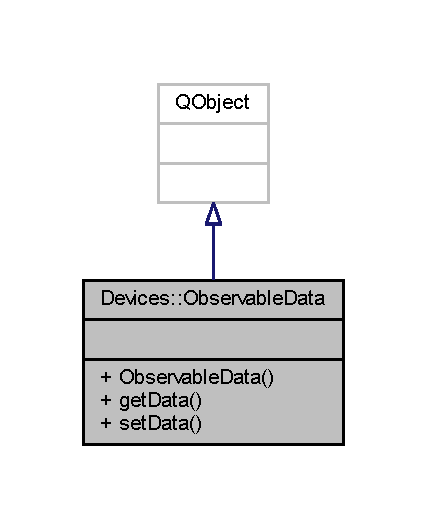
\includegraphics[width=205pt]{da/db4/class_devices_1_1_observable_data__inherit__graph}
\end{center}
\end{figure}


Collaboration diagram for Devices\+:\+:Observable\+Data\+:\nopagebreak
\begin{figure}[H]
\begin{center}
\leavevmode
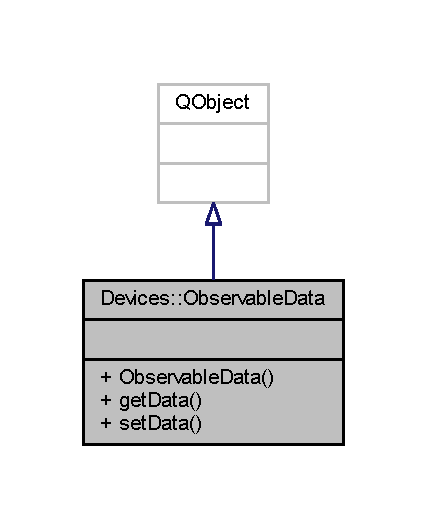
\includegraphics[width=205pt]{d2/d78/class_devices_1_1_observable_data__coll__graph}
\end{center}
\end{figure}
\subsection*{Public Member Functions}
\begin{DoxyCompactItemize}
\item 
\mbox{\Hypertarget{class_devices_1_1_observable_data_abb504c2ef0d30bcdf837d0d65ccb2051}\label{class_devices_1_1_observable_data_abb504c2ef0d30bcdf837d0d65ccb2051}} 
{\bfseries Observable\+Data} (Q\+Object $\ast$parent=nullptr)
\item 
\mbox{\Hypertarget{class_devices_1_1_observable_data_a184c8f851ca0e0f527c7d4efea81b324}\label{class_devices_1_1_observable_data_a184c8f851ca0e0f527c7d4efea81b324}} 
Q\+String {\bfseries get\+Data} () const
\item 
\mbox{\Hypertarget{class_devices_1_1_observable_data_a679da32e456f440f34131c807da3fbfd}\label{class_devices_1_1_observable_data_a679da32e456f440f34131c807da3fbfd}} 
void {\bfseries set\+Data} (const Q\+String \&value)
\end{DoxyCompactItemize}


\subsection{Detailed Description}


Definition at line 11 of file observabledata.\+h.



The documentation for this class was generated from the following files\+:\begin{DoxyCompactItemize}
\item 
object-\/detector/src/\+Devices\+Interfaces/\+Device\+Handler/observabledata.\+h\item 
object-\/detector/src/\+Devices\+Interfaces/\+Device\+Handler/observabledata.\+cpp\end{DoxyCompactItemize}

\hypertarget{class_devices_1_1_observer}{}\section{Devices\+:\+:Observer Class Reference}
\label{class_devices_1_1_observer}\index{Devices\+::\+Observer@{Devices\+::\+Observer}}


Inheritance diagram for Devices\+:\+:Observer\+:\nopagebreak
\begin{figure}[H]
\begin{center}
\leavevmode
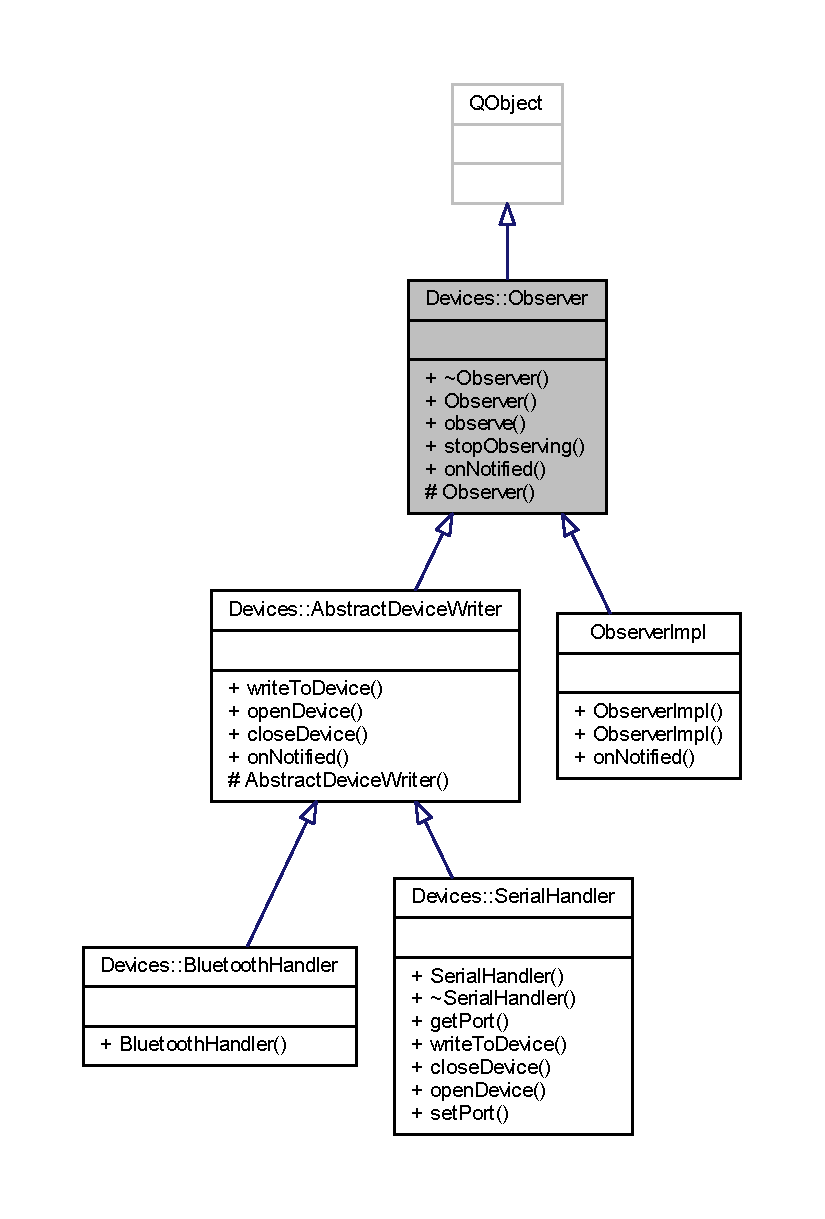
\includegraphics[width=350pt]{db/d46/class_devices_1_1_observer__inherit__graph}
\end{center}
\end{figure}


Collaboration diagram for Devices\+:\+:Observer\+:\nopagebreak
\begin{figure}[H]
\begin{center}
\leavevmode
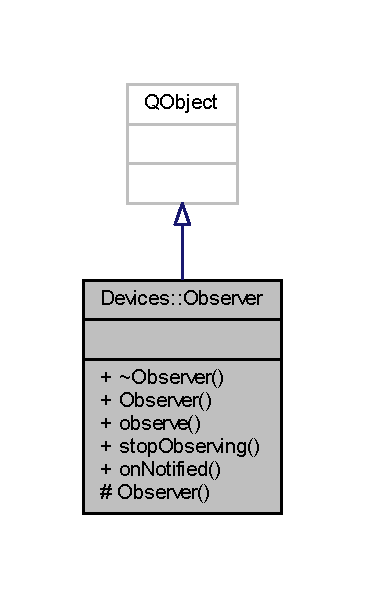
\includegraphics[width=175pt]{db/d51/class_devices_1_1_observer__coll__graph}
\end{center}
\end{figure}
\subsection*{Classes}
\begin{DoxyCompactItemize}
\item 
class {\bfseries \+\_\+\+Observer\+Impl}
\end{DoxyCompactItemize}
\subsection*{Public Slots}
\begin{DoxyCompactItemize}
\item 
\mbox{\Hypertarget{class_devices_1_1_observer_a4d3064deb1916b289a653862e0b0c141}\label{class_devices_1_1_observer_a4d3064deb1916b289a653862e0b0c141}} 
void {\bfseries observe} (\hyperlink{class_devices_1_1_subject}{Subject} $\ast$sub)
\item 
\mbox{\Hypertarget{class_devices_1_1_observer_a25201bb468d521bd5789c94ec08bc14c}\label{class_devices_1_1_observer_a25201bb468d521bd5789c94ec08bc14c}} 
void {\bfseries stop\+Observing} (\hyperlink{class_devices_1_1_subject}{Subject} $\ast$sub)
\item 
\mbox{\Hypertarget{class_devices_1_1_observer_a1dba681f223e67c2660d422cc4e7c6b5}\label{class_devices_1_1_observer_a1dba681f223e67c2660d422cc4e7c6b5}} 
virtual void {\bfseries on\+Notified} (const \hyperlink{class_devices_1_1_observable_data}{Observable\+Data} \&dt)=0
\end{DoxyCompactItemize}
\subsection*{Public Member Functions}
\begin{DoxyCompactItemize}
\item 
\mbox{\Hypertarget{class_devices_1_1_observer_a749229c39b82fb5c5ece5eaa4f4be4bc}\label{class_devices_1_1_observer_a749229c39b82fb5c5ece5eaa4f4be4bc}} 
{\bfseries Observer} (const \hyperlink{class_devices_1_1_observer}{Observer} \&)=default
\end{DoxyCompactItemize}
\subsection*{Protected Member Functions}
\begin{DoxyCompactItemize}
\item 
\mbox{\Hypertarget{class_devices_1_1_observer_a535c8656871306792a63d03c0eda96c8}\label{class_devices_1_1_observer_a535c8656871306792a63d03c0eda96c8}} 
{\bfseries Observer} (Q\+Object $\ast$parent=nullptr)
\end{DoxyCompactItemize}


The documentation for this class was generated from the following files\+:\begin{DoxyCompactItemize}
\item 
src/\+Object\+Detection/\+Devices\+Interfaces/\+Device\+Handler/observer.\+h\item 
src/\+Object\+Detection/\+Devices\+Interfaces/\+Device\+Handler/observer.\+cpp\end{DoxyCompactItemize}

\hypertarget{class_observer_impl}{}\section{Observer\+Impl Class Reference}
\label{class_observer_impl}\index{Observer\+Impl@{Observer\+Impl}}


Inheritance diagram for Observer\+Impl\+:\nopagebreak
\begin{figure}[H]
\begin{center}
\leavevmode
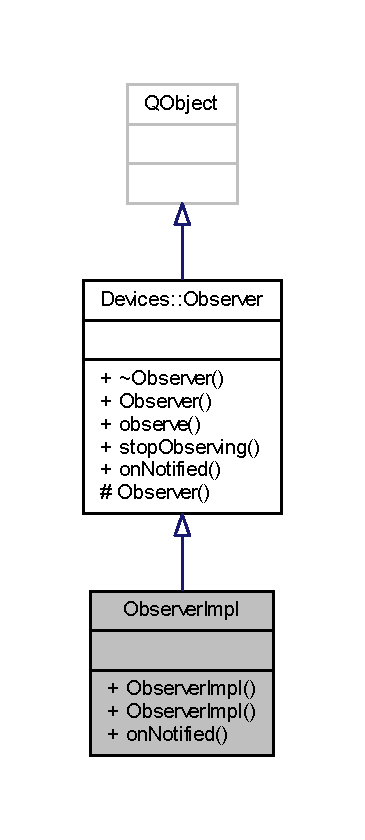
\includegraphics[width=175pt]{d4/d94/class_observer_impl__inherit__graph}
\end{center}
\end{figure}


Collaboration diagram for Observer\+Impl\+:\nopagebreak
\begin{figure}[H]
\begin{center}
\leavevmode
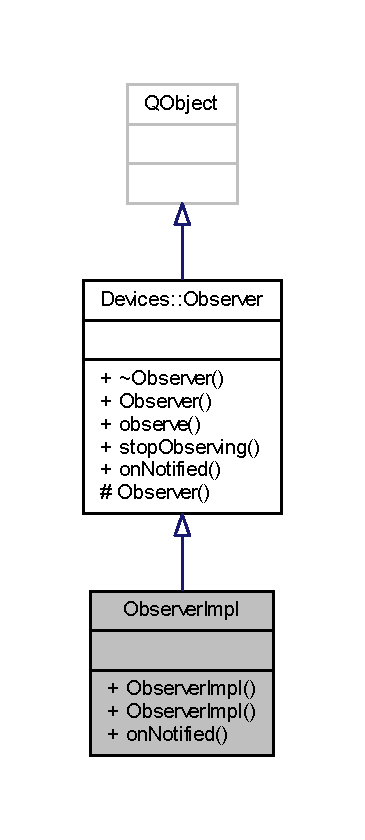
\includegraphics[width=175pt]{d4/de4/class_observer_impl__coll__graph}
\end{center}
\end{figure}
\subsection*{Public Slots}
\begin{DoxyCompactItemize}
\item 
\mbox{\Hypertarget{class_observer_impl_a1080d75c918e6d957749d21fe91b4ab8}\label{class_observer_impl_a1080d75c918e6d957749d21fe91b4ab8}} 
virtual void {\bfseries on\+Notified} (const \hyperlink{class_devices_1_1_observable_data}{Observable\+Data} \&dt) override
\end{DoxyCompactItemize}
\subsection*{Public Member Functions}
\begin{DoxyCompactItemize}
\item 
\mbox{\Hypertarget{class_observer_impl_a9fa47173043c11d1c3aa064080adebb4}\label{class_observer_impl_a9fa47173043c11d1c3aa064080adebb4}} 
{\bfseries Observer\+Impl} (Q\+Object $\ast$parent)
\item 
\mbox{\Hypertarget{class_observer_impl_af8f93e3842c3d9f8d9bd9cbf6c2964a3}\label{class_observer_impl_af8f93e3842c3d9f8d9bd9cbf6c2964a3}} 
{\bfseries Observer\+Impl} (const \hyperlink{class_observer_impl}{Observer\+Impl} \&)=default
\end{DoxyCompactItemize}
\subsection*{Additional Inherited Members}


The documentation for this class was generated from the following files\+:\begin{DoxyCompactItemize}
\item 
src/\+Object\+Detection/\+Devices\+Interfaces/\+Tests/\+Test\+Observer\+Subject/observerimpl.\+h\item 
src/\+Object\+Detection/\+Devices\+Interfaces/\+Tests/\+Test\+Observer\+Subject/observerimpl.\+cpp\end{DoxyCompactItemize}

\hypertarget{class_devices_1_1_serial_handler}{}\section{Devices\+:\+:Serial\+Handler Class Reference}
\label{class_devices_1_1_serial_handler}\index{Devices\+::\+Serial\+Handler@{Devices\+::\+Serial\+Handler}}


Inheritance diagram for Devices\+:\+:Serial\+Handler\+:\nopagebreak
\begin{figure}[H]
\begin{center}
\leavevmode
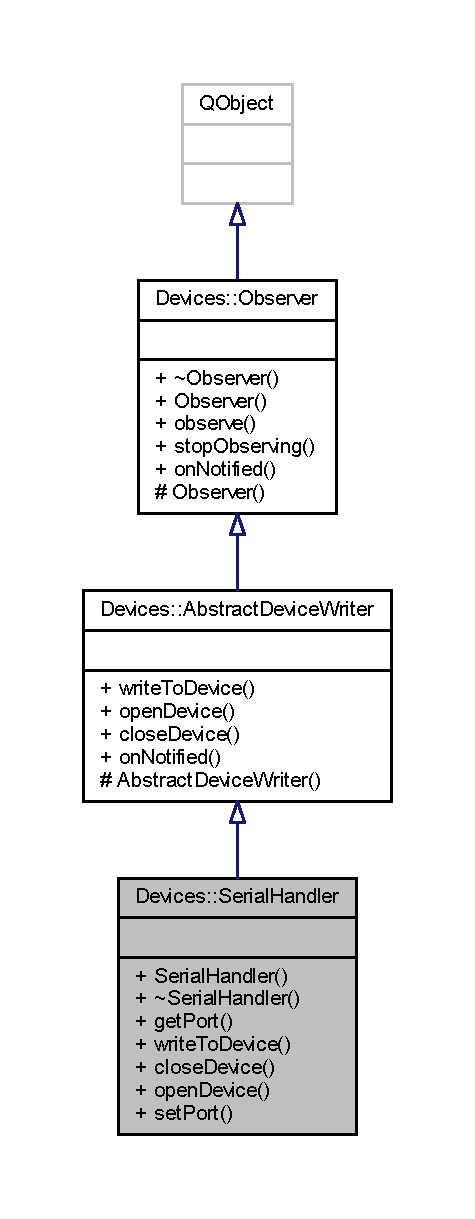
\includegraphics[height=550pt]{d2/dc5/class_devices_1_1_serial_handler__inherit__graph}
\end{center}
\end{figure}


Collaboration diagram for Devices\+:\+:Serial\+Handler\+:\nopagebreak
\begin{figure}[H]
\begin{center}
\leavevmode
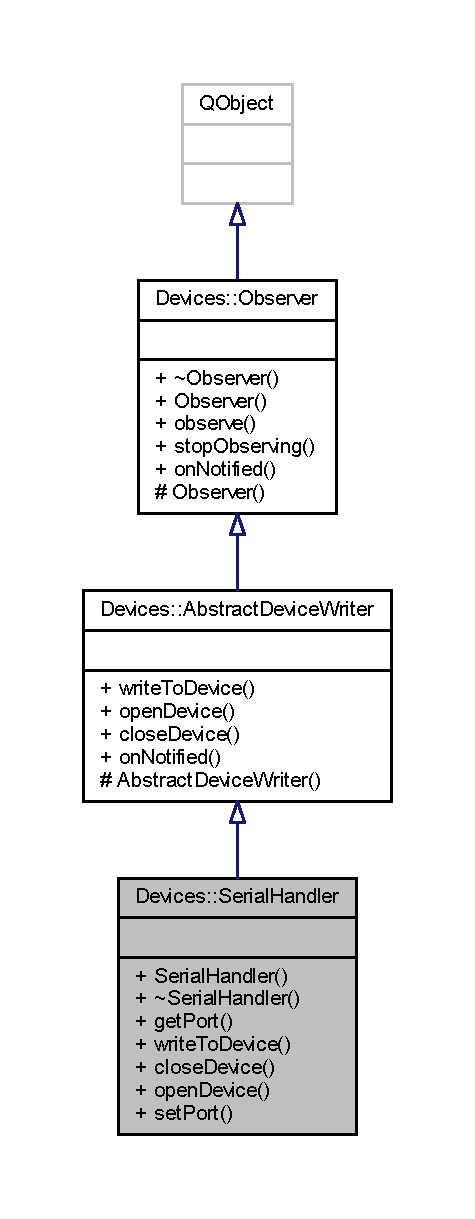
\includegraphics[height=550pt]{df/d83/class_devices_1_1_serial_handler__coll__graph}
\end{center}
\end{figure}
\subsection*{Classes}
\begin{DoxyCompactItemize}
\item 
class {\bfseries \+\_\+\+Serial\+Handler\+Impl}
\end{DoxyCompactItemize}
\subsection*{Public Slots}
\begin{DoxyCompactItemize}
\item 
\mbox{\Hypertarget{class_devices_1_1_serial_handler_aefd1562bc2b86e3ee7bac6df61d1b9b8}\label{class_devices_1_1_serial_handler_aefd1562bc2b86e3ee7bac6df61d1b9b8}} 
void {\bfseries set\+Port} (Q\+Serial\+Port $\ast$port)
\end{DoxyCompactItemize}
\subsection*{Public Member Functions}
\begin{DoxyCompactItemize}
\item 
\mbox{\Hypertarget{class_devices_1_1_serial_handler_a047b7ad42754bbfdad560af14de10285}\label{class_devices_1_1_serial_handler_a047b7ad42754bbfdad560af14de10285}} 
{\bfseries Serial\+Handler} (Q\+Object $\ast$parent=nullptr)
\item 
\mbox{\Hypertarget{class_devices_1_1_serial_handler_aed9d868caf3a381b186632c79548c575}\label{class_devices_1_1_serial_handler_aed9d868caf3a381b186632c79548c575}} 
Q\+Serial\+Port $\ast$ {\bfseries get\+Port} ()
\item 
\mbox{\Hypertarget{class_devices_1_1_serial_handler_a0deffd7d3589dfae6ff08a185820c20a}\label{class_devices_1_1_serial_handler_a0deffd7d3589dfae6ff08a185820c20a}} 
virtual void {\bfseries write\+To\+Device} (const Q\+String \&str) override
\item 
\mbox{\Hypertarget{class_devices_1_1_serial_handler_a2d1b4bc42515a9c734cc1fa78b52c193}\label{class_devices_1_1_serial_handler_a2d1b4bc42515a9c734cc1fa78b52c193}} 
virtual void {\bfseries close\+Device} () override
\item 
\mbox{\Hypertarget{class_devices_1_1_serial_handler_a955a72ed31a63f73c9c0aea463e97386}\label{class_devices_1_1_serial_handler_a955a72ed31a63f73c9c0aea463e97386}} 
virtual void {\bfseries open\+Device} () override
\end{DoxyCompactItemize}
\subsection*{Additional Inherited Members}


\subsection{Detailed Description}


Definition at line 14 of file serialhandler.\+h.



The documentation for this class was generated from the following files\+:\begin{DoxyCompactItemize}
\item 
object-\/detector/src/\+Devices\+Interfaces/\+Device\+Handler/\+Serial/serialhandler.\+h\item 
object-\/detector/src/\+Devices\+Interfaces/\+Device\+Handler/\+Serial/serialhandler.\+cpp\end{DoxyCompactItemize}

\hypertarget{class_devices_1_1_subject}{}\section{Devices\+:\+:Subject Class Reference}
\label{class_devices_1_1_subject}\index{Devices\+::\+Subject@{Devices\+::\+Subject}}


Inheritance diagram for Devices\+:\+:Subject\+:\nopagebreak
\begin{figure}[H]
\begin{center}
\leavevmode
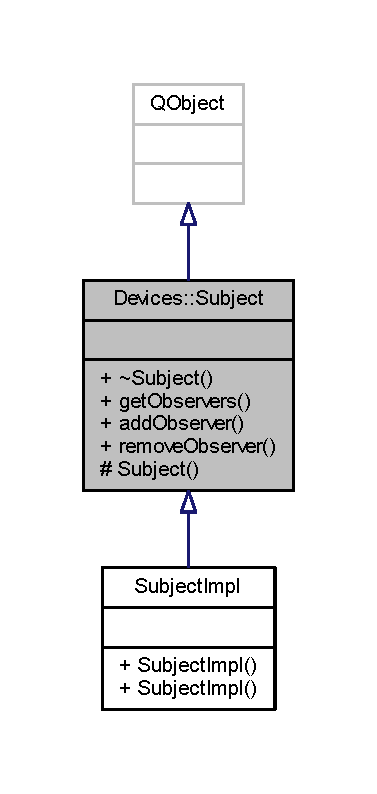
\includegraphics[width=181pt]{dd/d45/class_devices_1_1_subject__inherit__graph}
\end{center}
\end{figure}


Collaboration diagram for Devices\+:\+:Subject\+:\nopagebreak
\begin{figure}[H]
\begin{center}
\leavevmode
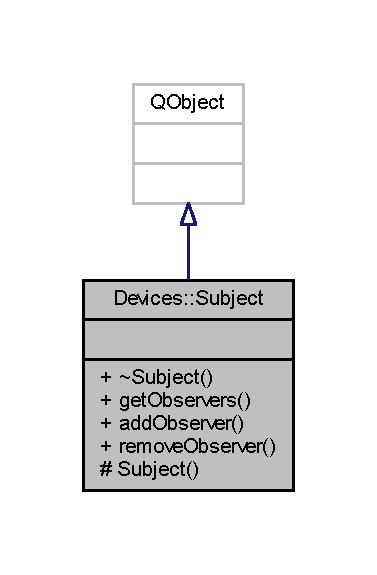
\includegraphics[width=181pt]{dd/dbf/class_devices_1_1_subject__coll__graph}
\end{center}
\end{figure}
\subsection*{Classes}
\begin{DoxyCompactItemize}
\item 
class {\bfseries \+\_\+\+Subject\+Impl}
\end{DoxyCompactItemize}
\subsection*{Public Slots}
\begin{DoxyCompactItemize}
\item 
\mbox{\Hypertarget{class_devices_1_1_subject_a7aec3567898fc9bbebdeba8a335029f4}\label{class_devices_1_1_subject_a7aec3567898fc9bbebdeba8a335029f4}} 
void {\bfseries add\+Observer} (\hyperlink{class_devices_1_1_observer}{Observer} $\ast$obs)
\item 
\mbox{\Hypertarget{class_devices_1_1_subject_a7cb918292445a292263e2e0f8e74903d}\label{class_devices_1_1_subject_a7cb918292445a292263e2e0f8e74903d}} 
void {\bfseries remove\+Observer} (\hyperlink{class_devices_1_1_observer}{Observer} $\ast$obs)
\end{DoxyCompactItemize}
\subsection*{Signals}
\begin{DoxyCompactItemize}
\item 
\mbox{\Hypertarget{class_devices_1_1_subject_a715b3a4513893d294229ee76f2ed3cbe}\label{class_devices_1_1_subject_a715b3a4513893d294229ee76f2ed3cbe}} 
void {\bfseries notify\+Observers} (const \hyperlink{class_devices_1_1_observable_data}{Observable\+Data} \&)
\end{DoxyCompactItemize}
\subsection*{Public Member Functions}
\begin{DoxyCompactItemize}
\item 
\mbox{\Hypertarget{class_devices_1_1_subject_adbc2b175f510857715682e571851b215}\label{class_devices_1_1_subject_adbc2b175f510857715682e571851b215}} 
std\+::vector$<$ \hyperlink{class_devices_1_1_observer}{Observer} $\ast$ $>$ {\bfseries get\+Observers} () const
\end{DoxyCompactItemize}
\subsection*{Protected Member Functions}
\begin{DoxyCompactItemize}
\item 
\mbox{\Hypertarget{class_devices_1_1_subject_ac78bedb24be6afb83b4fa334badc549b}\label{class_devices_1_1_subject_ac78bedb24be6afb83b4fa334badc549b}} 
{\bfseries Subject} (Q\+Object $\ast$parent=nullptr)
\end{DoxyCompactItemize}


The documentation for this class was generated from the following files\+:\begin{DoxyCompactItemize}
\item 
src/\+Object\+Detection/\+Devices\+Interfaces/\+Device\+Handler/subject.\+h\item 
src/\+Object\+Detection/\+Devices\+Interfaces/\+Device\+Handler/subject.\+cpp\end{DoxyCompactItemize}

\hypertarget{class_subject_impl}{}\section{Subject\+Impl Class Reference}
\label{class_subject_impl}\index{Subject\+Impl@{Subject\+Impl}}


Inheritance diagram for Subject\+Impl\+:\nopagebreak
\begin{figure}[H]
\begin{center}
\leavevmode
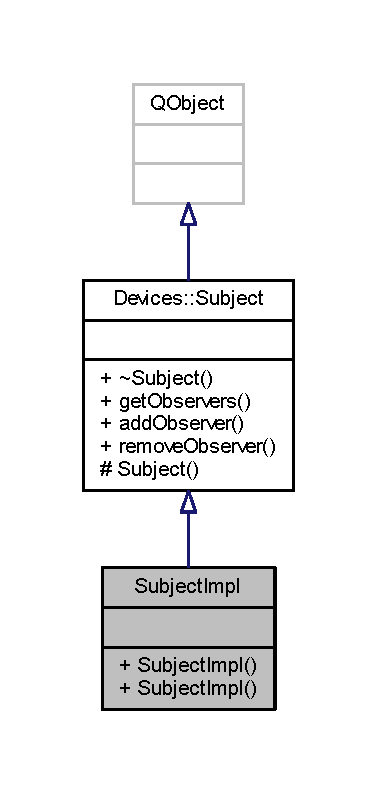
\includegraphics[width=181pt]{de/d5e/class_subject_impl__inherit__graph}
\end{center}
\end{figure}


Collaboration diagram for Subject\+Impl\+:\nopagebreak
\begin{figure}[H]
\begin{center}
\leavevmode
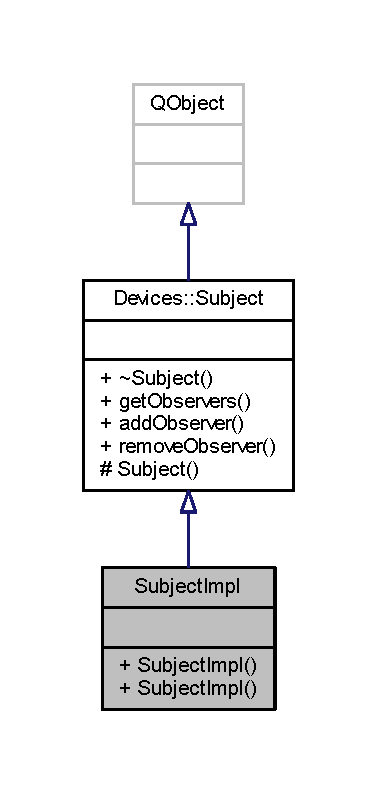
\includegraphics[width=181pt]{d9/d7f/class_subject_impl__coll__graph}
\end{center}
\end{figure}
\subsection*{Public Member Functions}
\begin{DoxyCompactItemize}
\item 
\mbox{\Hypertarget{class_subject_impl_a8cd9bc47afd82f8a957c7a56154cd528}\label{class_subject_impl_a8cd9bc47afd82f8a957c7a56154cd528}} 
{\bfseries Subject\+Impl} (Q\+Object $\ast$parent=nullptr)
\item 
\mbox{\Hypertarget{class_subject_impl_a62f084a4816178f5f74514f95af03515}\label{class_subject_impl_a62f084a4816178f5f74514f95af03515}} 
{\bfseries Subject\+Impl} (const \hyperlink{class_subject_impl}{Subject\+Impl} \&)=default
\end{DoxyCompactItemize}
\subsection*{Additional Inherited Members}


The documentation for this class was generated from the following files\+:\begin{DoxyCompactItemize}
\item 
src/\+Object\+Detection/\+Devices\+Interfaces/\+Tests/\+Test\+Observer\+Subject/subjectimpl.\+h\item 
src/\+Object\+Detection/\+Devices\+Interfaces/\+Tests/\+Test\+Observer\+Subject/subjectimpl.\+cpp\end{DoxyCompactItemize}

\hypertarget{class_test_observer_subject_test}{}\section{Test\+Observer\+Subject\+Test Class Reference}
\label{class_test_observer_subject_test}\index{Test\+Observer\+Subject\+Test@{Test\+Observer\+Subject\+Test}}


Inheritance diagram for Test\+Observer\+Subject\+Test\+:\nopagebreak
\begin{figure}[H]
\begin{center}
\leavevmode
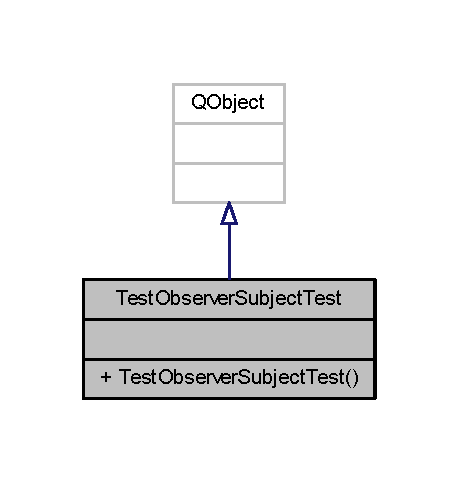
\includegraphics[width=220pt]{d5/d93/class_test_observer_subject_test__inherit__graph}
\end{center}
\end{figure}


Collaboration diagram for Test\+Observer\+Subject\+Test\+:\nopagebreak
\begin{figure}[H]
\begin{center}
\leavevmode
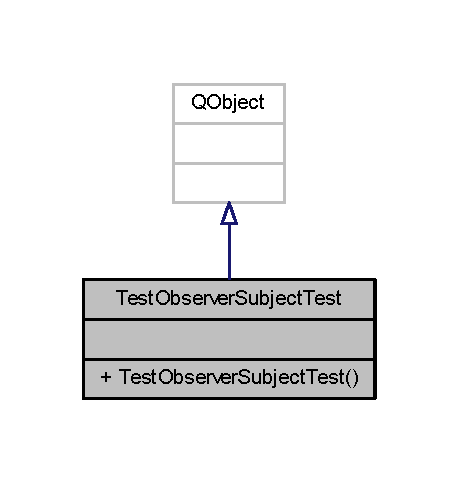
\includegraphics[width=220pt]{d6/d96/class_test_observer_subject_test__coll__graph}
\end{center}
\end{figure}


\subsection{Detailed Description}


Definition at line 11 of file tst\+\_\+testobserversubjecttest.\+cpp.



The documentation for this class was generated from the following file\+:\begin{DoxyCompactItemize}
\item 
object-\/detector/src/\+Devices\+Interfaces/\+Tests/\+Test\+Observer\+Subject/tst\+\_\+testobserversubjecttest.\+cpp\end{DoxyCompactItemize}

\hypertarget{class_test_work}{}\section{Test\+Work Class Reference}
\label{class_test_work}\index{Test\+Work@{Test\+Work}}


Inheritance diagram for Test\+Work\+:\nopagebreak
\begin{figure}[H]
\begin{center}
\leavevmode
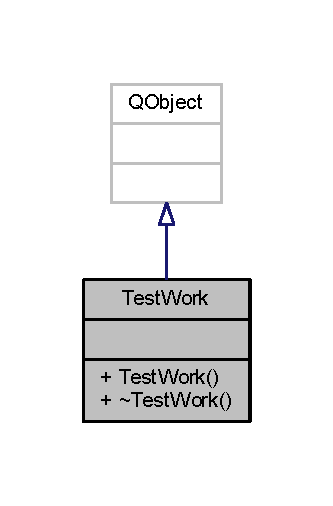
\includegraphics[width=160pt]{d8/dc0/class_test_work__inherit__graph}
\end{center}
\end{figure}


Collaboration diagram for Test\+Work\+:\nopagebreak
\begin{figure}[H]
\begin{center}
\leavevmode
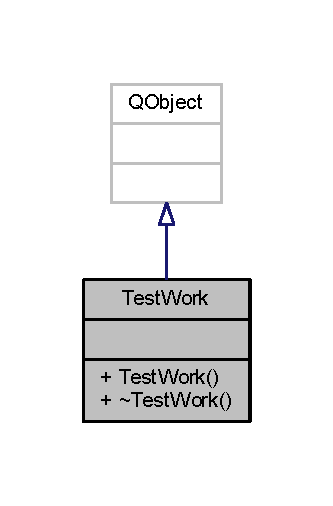
\includegraphics[width=160pt]{d0/d00/class_test_work__coll__graph}
\end{center}
\end{figure}


\subsection{Detailed Description}


Definition at line 6 of file tst\+\_\+testwork.\+cpp.



The documentation for this class was generated from the following file\+:\begin{DoxyCompactItemize}
\item 
object-\/detector/src/\+Circle\+Detector/\+Tests/\+Detect\+Color\+Test/tst\+\_\+testwork.\+cpp\end{DoxyCompactItemize}

\hypertarget{class_ui___main_window}{}\section{Ui\+\_\+\+Main\+Window Class Reference}
\label{class_ui___main_window}\index{Ui\+\_\+\+Main\+Window@{Ui\+\_\+\+Main\+Window}}


Inheritance diagram for Ui\+\_\+\+Main\+Window\+:\nopagebreak
\begin{figure}[H]
\begin{center}
\leavevmode
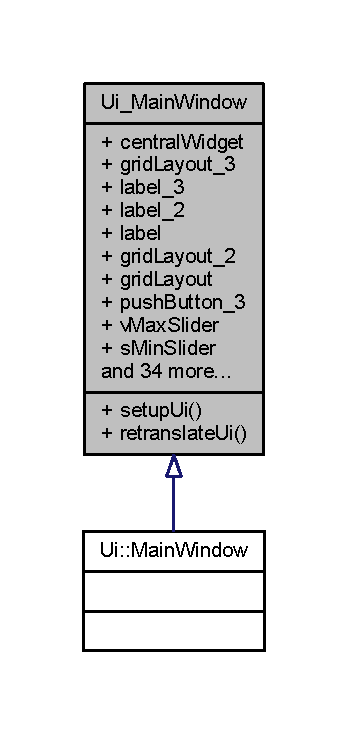
\includegraphics[width=177pt]{dd/df1/class_ui___main_window__inherit__graph}
\end{center}
\end{figure}


Collaboration diagram for Ui\+\_\+\+Main\+Window\+:\nopagebreak
\begin{figure}[H]
\begin{center}
\leavevmode
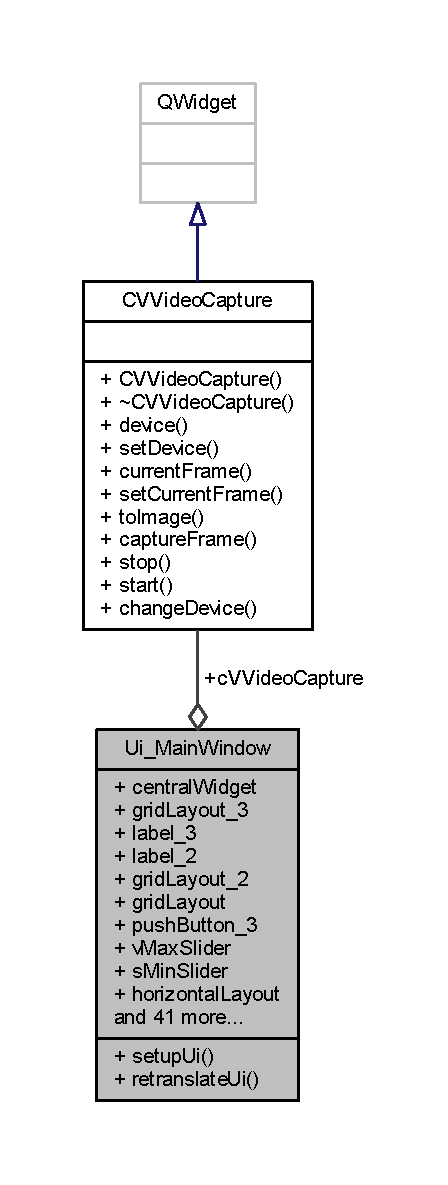
\includegraphics[height=550pt]{d5/d21/class_ui___main_window__coll__graph}
\end{center}
\end{figure}
\subsection*{Public Member Functions}
\begin{DoxyCompactItemize}
\item 
\mbox{\Hypertarget{class_ui___main_window_acf4a0872c4c77d8f43a2ec66ed849b58}\label{class_ui___main_window_acf4a0872c4c77d8f43a2ec66ed849b58}} 
void {\bfseries setup\+Ui} (Q\+Main\+Window $\ast$\hyperlink{class_main_window}{Main\+Window})
\item 
\mbox{\Hypertarget{class_ui___main_window_a097dd160c3534a204904cb374412c618}\label{class_ui___main_window_a097dd160c3534a204904cb374412c618}} 
void {\bfseries retranslate\+Ui} (Q\+Main\+Window $\ast$\hyperlink{class_main_window}{Main\+Window})
\end{DoxyCompactItemize}
\subsection*{Public Attributes}
\begin{DoxyCompactItemize}
\item 
\mbox{\Hypertarget{class_ui___main_window_a30075506c2116c3ed4ff25e07ae75f81}\label{class_ui___main_window_a30075506c2116c3ed4ff25e07ae75f81}} 
Q\+Widget $\ast$ {\bfseries central\+Widget}
\item 
\mbox{\Hypertarget{class_ui___main_window_af42ea7d4c2e893181caad21e28166932}\label{class_ui___main_window_af42ea7d4c2e893181caad21e28166932}} 
Q\+Grid\+Layout $\ast$ {\bfseries grid\+Layout\+\_\+3}
\item 
\mbox{\Hypertarget{class_ui___main_window_a0376fd90247280e7c7957cc70628708c}\label{class_ui___main_window_a0376fd90247280e7c7957cc70628708c}} 
Q\+Label $\ast$ {\bfseries label\+\_\+3}
\item 
\mbox{\Hypertarget{class_ui___main_window_a2e2516d755e4dd53fc905dabddf2738a}\label{class_ui___main_window_a2e2516d755e4dd53fc905dabddf2738a}} 
Q\+Label $\ast$ {\bfseries label\+\_\+2}
\item 
\mbox{\Hypertarget{class_ui___main_window_a6b2a0c5f7e8ff2a87134908dd770d2d2}\label{class_ui___main_window_a6b2a0c5f7e8ff2a87134908dd770d2d2}} 
Q\+Grid\+Layout $\ast$ {\bfseries grid\+Layout\+\_\+2}
\item 
\mbox{\Hypertarget{class_ui___main_window_a525ed3c5fe0784ac502ee222fba4e205}\label{class_ui___main_window_a525ed3c5fe0784ac502ee222fba4e205}} 
Q\+Grid\+Layout $\ast$ {\bfseries grid\+Layout}
\item 
\mbox{\Hypertarget{class_ui___main_window_ac92cce0478c1025ace05ff4f8870bb1c}\label{class_ui___main_window_ac92cce0478c1025ace05ff4f8870bb1c}} 
Q\+Push\+Button $\ast$ {\bfseries push\+Button\+\_\+3}
\item 
\mbox{\Hypertarget{class_ui___main_window_a818f37cd929add75563bc4f2552abd15}\label{class_ui___main_window_a818f37cd929add75563bc4f2552abd15}} 
Q\+Slider $\ast$ {\bfseries v\+Max\+Slider}
\item 
\mbox{\Hypertarget{class_ui___main_window_a875bd6b40387a665b8d3cc2ae1d273a1}\label{class_ui___main_window_a875bd6b40387a665b8d3cc2ae1d273a1}} 
Q\+Slider $\ast$ {\bfseries s\+Min\+Slider}
\item 
\mbox{\Hypertarget{class_ui___main_window_acd6fdc9ebacc4b25b834162380d75ce8}\label{class_ui___main_window_acd6fdc9ebacc4b25b834162380d75ce8}} 
Q\+H\+Box\+Layout $\ast$ {\bfseries horizontal\+Layout}
\item 
\mbox{\Hypertarget{class_ui___main_window_a4440506b5624f4e8740602f76417944e}\label{class_ui___main_window_a4440506b5624f4e8740602f76417944e}} 
Q\+Label $\ast$ {\bfseries radius\+Label}
\item 
\mbox{\Hypertarget{class_ui___main_window_ac65c7239c6905578a56486867e06a43f}\label{class_ui___main_window_ac65c7239c6905578a56486867e06a43f}} 
Q\+Label $\ast$ {\bfseries y\+Label\+Center}
\item 
\mbox{\Hypertarget{class_ui___main_window_a5a64a858f438e5bdedc15642f11a64a0}\label{class_ui___main_window_a5a64a858f438e5bdedc15642f11a64a0}} 
Q\+Label $\ast$ {\bfseries x\+Center\+Label}
\item 
\mbox{\Hypertarget{class_ui___main_window_abb28acde35ffce4d0e6152579df2cbc3}\label{class_ui___main_window_abb28acde35ffce4d0e6152579df2cbc3}} 
Q\+Group\+Box $\ast$ {\bfseries group\+Box\+\_\+2}
\item 
\mbox{\Hypertarget{class_ui___main_window_a0c01bad60d9f422a1258e710635a2f65}\label{class_ui___main_window_a0c01bad60d9f422a1258e710635a2f65}} 
Q\+V\+Box\+Layout $\ast$ {\bfseries vertical\+Layout\+\_\+2}
\item 
\mbox{\Hypertarget{class_ui___main_window_a3068d27ac53bbf52528fcf4ca962f99e}\label{class_ui___main_window_a3068d27ac53bbf52528fcf4ca962f99e}} 
Q\+Slider $\ast$ {\bfseries min\+Dist\+Slider}
\item 
\mbox{\Hypertarget{class_ui___main_window_a151239c9ccdd2e422dc31982d353c058}\label{class_ui___main_window_a151239c9ccdd2e422dc31982d353c058}} 
Q\+Slider $\ast$ {\bfseries param1\+Slider}
\item 
\mbox{\Hypertarget{class_ui___main_window_a8abf290436a994da52256687b988e73a}\label{class_ui___main_window_a8abf290436a994da52256687b988e73a}} 
Q\+Slider $\ast$ {\bfseries param2\+Slider}
\item 
\mbox{\Hypertarget{class_ui___main_window_a59a7d8124bce933d63f53f2153d447b4}\label{class_ui___main_window_a59a7d8124bce933d63f53f2153d447b4}} 
Q\+Push\+Button $\ast$ {\bfseries push\+Button\+\_\+2}
\item 
\mbox{\Hypertarget{class_ui___main_window_a741b4db05a469f9f55a3dd0fbe0dfeaf}\label{class_ui___main_window_a741b4db05a469f9f55a3dd0fbe0dfeaf}} 
Q\+Slider $\ast$ {\bfseries circle\+Thickness\+Slider}
\item 
\mbox{\Hypertarget{class_ui___main_window_afea65459525c1bd69676decbf5cdeaac}\label{class_ui___main_window_afea65459525c1bd69676decbf5cdeaac}} 
Q\+Slider $\ast$ {\bfseries v\+Min\+Slider}
\item 
\mbox{\Hypertarget{class_ui___main_window_aeb4aae1abf447280aba3c5999d2a324e}\label{class_ui___main_window_aeb4aae1abf447280aba3c5999d2a324e}} 
Q\+Slider $\ast$ {\bfseries s\+Max\+Slider}
\item 
\mbox{\Hypertarget{class_ui___main_window_a8dd8d488f868d1950ed3cb5c7d443833}\label{class_ui___main_window_a8dd8d488f868d1950ed3cb5c7d443833}} 
Q\+Slider $\ast$ {\bfseries h\+Min\+Slider}
\item 
\mbox{\Hypertarget{class_ui___main_window_ad332d93084584930878f1daf5f84cdbf}\label{class_ui___main_window_ad332d93084584930878f1daf5f84cdbf}} 
Q\+Push\+Button $\ast$ {\bfseries push\+Button}
\item 
\mbox{\Hypertarget{class_ui___main_window_adc7332ba9b0cbfdc99f8124c9a34f9d0}\label{class_ui___main_window_adc7332ba9b0cbfdc99f8124c9a34f9d0}} 
Q\+Slider $\ast$ {\bfseries h\+Max\+Slider}
\item 
\mbox{\Hypertarget{class_ui___main_window_a78c7e10730b43c6700cd7216911ed76a}\label{class_ui___main_window_a78c7e10730b43c6700cd7216911ed76a}} 
Q\+Label $\ast$ {\bfseries label\+\_\+4}
\item 
\mbox{\Hypertarget{class_ui___main_window_a663f728e6244926a795c6e6892673b1d}\label{class_ui___main_window_a663f728e6244926a795c6e6892673b1d}} 
Q\+Label $\ast$ {\bfseries label\+\_\+6}
\item 
\mbox{\Hypertarget{class_ui___main_window_a13936e6f18b1c90402b3c7a3c92b6cdb}\label{class_ui___main_window_a13936e6f18b1c90402b3c7a3c92b6cdb}} 
Q\+Label $\ast$ {\bfseries label\+\_\+7}
\item 
\mbox{\Hypertarget{class_ui___main_window_ad6bab8fb8903b8f41afea1218ee52695}\label{class_ui___main_window_ad6bab8fb8903b8f41afea1218ee52695}} 
Q\+Label $\ast$ {\bfseries label\+\_\+5}
\item 
\mbox{\Hypertarget{class_ui___main_window_af183bfbfb9f38bbdd60caf92b15e23dc}\label{class_ui___main_window_af183bfbfb9f38bbdd60caf92b15e23dc}} 
Q\+Label $\ast$ {\bfseries label\+\_\+8}
\item 
\mbox{\Hypertarget{class_ui___main_window_a6c286be5261968e19663fc8ccef62209}\label{class_ui___main_window_a6c286be5261968e19663fc8ccef62209}} 
Q\+Spin\+Box $\ast$ {\bfseries spin\+Box\+\_\+3}
\item 
\mbox{\Hypertarget{class_ui___main_window_ab670e9aaf9844eff45b10bcb409bae91}\label{class_ui___main_window_ab670e9aaf9844eff45b10bcb409bae91}} 
Q\+Spin\+Box $\ast$ {\bfseries spin\+Box\+\_\+4}
\item 
\mbox{\Hypertarget{class_ui___main_window_ad8232de6059b8abe59b79973399640e5}\label{class_ui___main_window_ad8232de6059b8abe59b79973399640e5}} 
Q\+Spin\+Box $\ast$ {\bfseries spin\+Box\+\_\+2}
\item 
\mbox{\Hypertarget{class_ui___main_window_a92db6f665478d959dd56a61fa0215838}\label{class_ui___main_window_a92db6f665478d959dd56a61fa0215838}} 
Q\+Spin\+Box $\ast$ {\bfseries spin\+Box\+\_\+5}
\item 
\mbox{\Hypertarget{class_ui___main_window_a2b43dc1718accf7a1f5c70e410cc7ee7}\label{class_ui___main_window_a2b43dc1718accf7a1f5c70e410cc7ee7}} 
Q\+Spin\+Box $\ast$ {\bfseries spin\+Box\+\_\+6}
\item 
\mbox{\Hypertarget{class_ui___main_window_a3f54feaa7edb2b4810acc4dc53b70e60}\label{class_ui___main_window_a3f54feaa7edb2b4810acc4dc53b70e60}} 
Q\+Spin\+Box $\ast$ {\bfseries spin\+Box\+\_\+7}
\item 
\mbox{\Hypertarget{class_ui___main_window_aef7cb3be8cecfc9aaf98f036a98781ce}\label{class_ui___main_window_aef7cb3be8cecfc9aaf98f036a98781ce}} 
Q\+Group\+Box $\ast$ {\bfseries group\+Box}
\item 
\mbox{\Hypertarget{class_ui___main_window_aecd96a04789fcfec3f98d80390ad8184}\label{class_ui___main_window_aecd96a04789fcfec3f98d80390ad8184}} 
Q\+V\+Box\+Layout $\ast$ {\bfseries vertical\+Layout}
\item 
\mbox{\Hypertarget{class_ui___main_window_a61269a10bc342763a5a51a93a235944d}\label{class_ui___main_window_a61269a10bc342763a5a51a93a235944d}} 
Q\+Radio\+Button $\ast$ {\bfseries radio\+Button}
\item 
\mbox{\Hypertarget{class_ui___main_window_aae7b8581981931a792a768767fbf755f}\label{class_ui___main_window_aae7b8581981931a792a768767fbf755f}} 
Q\+Radio\+Button $\ast$ {\bfseries radio\+Button\+\_\+2}
\item 
\mbox{\Hypertarget{class_ui___main_window_a279bf4f986f7426fcede6af133190055}\label{class_ui___main_window_a279bf4f986f7426fcede6af133190055}} 
Q\+Radio\+Button $\ast$ {\bfseries radio\+Button\+\_\+3}
\item 
\mbox{\Hypertarget{class_ui___main_window_ac410fb505e22ae3bf3aefed954d9b961}\label{class_ui___main_window_ac410fb505e22ae3bf3aefed954d9b961}} 
Q\+Radio\+Button $\ast$ {\bfseries radio\+Button\+\_\+4}
\item 
\mbox{\Hypertarget{class_ui___main_window_a4e4c33d607d38a4e5bba06ae373b72a3}\label{class_ui___main_window_a4e4c33d607d38a4e5bba06ae373b72a3}} 
Q\+Slider $\ast$ {\bfseries dil\+Slider}
\item 
\mbox{\Hypertarget{class_ui___main_window_adafdad7c065227c5d14b68d75789cbe2}\label{class_ui___main_window_adafdad7c065227c5d14b68d75789cbe2}} 
Q\+Push\+Button $\ast$ {\bfseries push\+Button\+\_\+5}
\item 
\mbox{\Hypertarget{class_ui___main_window_a5ee2488c049a177071c1485b4138e113}\label{class_ui___main_window_a5ee2488c049a177071c1485b4138e113}} 
Q\+Spin\+Box $\ast$ {\bfseries spin\+Box}
\item 
\mbox{\Hypertarget{class_ui___main_window_a38b8a4b887f3b58e2a49e7905ae6f1f0}\label{class_ui___main_window_a38b8a4b887f3b58e2a49e7905ae6f1f0}} 
Q\+V\+Box\+Layout $\ast$ {\bfseries vertical\+Layout\+\_\+3}
\item 
\mbox{\Hypertarget{class_ui___main_window_a3f4332a5b5e82f676f25ec3148c1c83c}\label{class_ui___main_window_a3f4332a5b5e82f676f25ec3148c1c83c}} 
Q\+Table\+View $\ast$ {\bfseries table\+View}
\item 
\mbox{\Hypertarget{class_ui___main_window_acb0b2f196dc2224f287b67594233297f}\label{class_ui___main_window_acb0b2f196dc2224f287b67594233297f}} 
Q\+Push\+Button $\ast$ {\bfseries push\+Button\+\_\+4}
\item 
\mbox{\Hypertarget{class_ui___main_window_a202ae5e4de2494091a0640f9e7a5bcd0}\label{class_ui___main_window_a202ae5e4de2494091a0640f9e7a5bcd0}} 
\hyperlink{class_c_v_video_capture}{C\+V\+Video\+Capture} $\ast$ {\bfseries c\+V\+Video\+Capture}
\item 
\mbox{\Hypertarget{class_ui___main_window_a2be1c24ec9adfca18e1dcc951931457f}\label{class_ui___main_window_a2be1c24ec9adfca18e1dcc951931457f}} 
Q\+Menu\+Bar $\ast$ {\bfseries menu\+Bar}
\item 
\mbox{\Hypertarget{class_ui___main_window_a5172877001c8c7b4e0f6de50421867d1}\label{class_ui___main_window_a5172877001c8c7b4e0f6de50421867d1}} 
Q\+Tool\+Bar $\ast$ {\bfseries main\+Tool\+Bar}
\item 
\mbox{\Hypertarget{class_ui___main_window_a50fa481337604bcc8bf68de18ab16ecd}\label{class_ui___main_window_a50fa481337604bcc8bf68de18ab16ecd}} 
Q\+Status\+Bar $\ast$ {\bfseries status\+Bar}
\end{DoxyCompactItemize}


\subsection{Detailed Description}


Definition at line 36 of file ui\+\_\+mainwindow.\+h.



The documentation for this class was generated from the following file\+:\begin{DoxyCompactItemize}
\item 
object-\/detector/src/\+View/\+Desktop\+View/\+View/ui\+\_\+mainwindow.\+h\end{DoxyCompactItemize}

\hypertarget{class_utilities_1_1_utils}{}\section{Utilities\+:\+:Utils Class Reference}
\label{class_utilities_1_1_utils}\index{Utilities\+::\+Utils@{Utilities\+::\+Utils}}


Inheritance diagram for Utilities\+:\+:Utils\+:\nopagebreak
\begin{figure}[H]
\begin{center}
\leavevmode
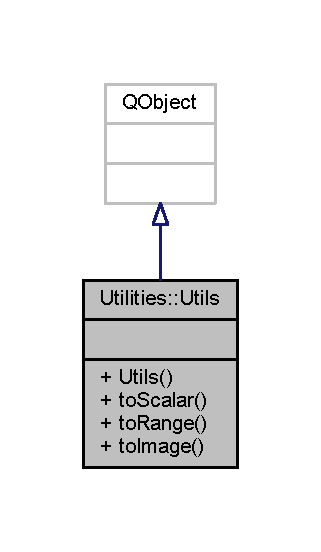
\includegraphics[width=154pt]{dc/d46/class_utilities_1_1_utils__inherit__graph}
\end{center}
\end{figure}


Collaboration diagram for Utilities\+:\+:Utils\+:\nopagebreak
\begin{figure}[H]
\begin{center}
\leavevmode
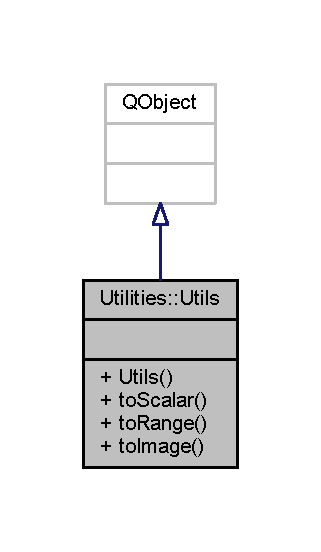
\includegraphics[width=154pt]{dd/db7/class_utilities_1_1_utils__coll__graph}
\end{center}
\end{figure}
\subsection*{Public Member Functions}
\begin{DoxyCompactItemize}
\item 
\mbox{\Hypertarget{class_utilities_1_1_utils_a2485caf868a56ee5a1f6052193fd722c}\label{class_utilities_1_1_utils_a2485caf868a56ee5a1f6052193fd722c}} 
{\bfseries Utils} (Q\+Object $\ast$parent=nullptr)
\end{DoxyCompactItemize}
\subsection*{Static Public Member Functions}
\begin{DoxyCompactItemize}
\item 
\mbox{\Hypertarget{class_utilities_1_1_utils_a3e2dc24f6e8bffb572a968015f070e3d}\label{class_utilities_1_1_utils_a3e2dc24f6e8bffb572a968015f070e3d}} 
static cv\+::\+Scalar {\bfseries to\+Scalar} (Q\+Color color)
\item 
\mbox{\Hypertarget{class_utilities_1_1_utils_a8049b798a16e83ac705fa3cda8340c7e}\label{class_utilities_1_1_utils_a8049b798a16e83ac705fa3cda8340c7e}} 
static std\+::tuple$<$ cv\+::\+Scalar, cv\+::\+Scalar $>$ {\bfseries to\+Range} (Q\+Color color)
\item 
\mbox{\Hypertarget{class_utilities_1_1_utils_ac8c1bcc2dd3d5bda38d1636bd92e5173}\label{class_utilities_1_1_utils_ac8c1bcc2dd3d5bda38d1636bd92e5173}} 
static Q\+Image {\bfseries to\+Image} (const cv\+::\+Mat \&m)
\end{DoxyCompactItemize}


\subsection{Detailed Description}


Definition at line 12 of file utils.\+h.



The documentation for this class was generated from the following files\+:\begin{DoxyCompactItemize}
\item 
object-\/detector/src/\+Utilities/\+Utils/\+Utilities/utils.\+h\item 
object-\/detector/src/\+Utilities/\+Utils/\+Utilities/utils.\+cpp\end{DoxyCompactItemize}

\hypertarget{class_utils}{}\section{Utils Class Reference}
\label{class_utils}\index{Utils@{Utils}}


Collaboration diagram for Utils\+:\nopagebreak
\begin{figure}[H]
\begin{center}
\leavevmode
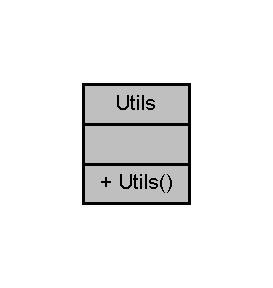
\includegraphics[width=131pt]{df/d3f/class_utils__coll__graph}
\end{center}
\end{figure}


The documentation for this class was generated from the following files\+:\begin{DoxyCompactItemize}
\item 
src/\+Object\+Detection/\+Utilities/\+Utils/utils.\+h\item 
src/\+Object\+Detection/\+Utilities/\+Utils/utils.\+cpp\end{DoxyCompactItemize}

%--- End generated contents ---

% Index
\backmatter
\newpage
\phantomsection
\clearemptydoublepage
\addcontentsline{toc}{chapter}{Index}
\printindex

\end{document}
